\documentclass{slides}
\usepackage{xspace}
\usepackage{nth}
\usepackage{fontawesome}
\usepackage{hyperref}
\hypersetup{
    colorlinks = true,
    urlcolor = blue
}

\title[Bayesian Inference]{Introducing Bayesian Inference}
\author[Andrews]{Mark Andrews \\ $\phantom{foo}$ \\ Psychology, Nottingham Trent University \\ $\phantom{foo}$ \\ \faEnvelopeO \  \texttt{mark.andrews@ntu.ac.uk} \\ $\phantom{foo}$ \\ \faTwitter \href{https://twitter.com/xmjandrews}{@xmjandrews}, \faTwitter \href{https://twitter.com/priorexposure}{@priorexposure}\\ $\phantom{foo}$ \\ \faGithub \ \url{https://github.com/lawsofthought/psbayes}}

\date{December, 2018}

\begin{document}
{
	\begin{frame}
		\titlepage
	\end{frame}
}


\begin{frame}
\frametitle{Inference in a Bernoulli Distribution}
\framesubtitle{e.g., inferring a coin's bias}

\vspace{\baselineskip}
\begin{quotation} \small \ldots Polish mathematicians Tomasz Gliszczynski and
	Waclaw Zawadowski\ldots spun a Belgian one euro coin 250 times,
	and found it landed heads up 140 times \ldots When tossed 250
	times, the one euro coin came up heads 139 times and tails 111.
	\ldots 
\end{quotation}
	\vspace{-\baselineskip}
\flushright{\small \emph{The Guardian}, January 4, 2002\footnote{ See
	\texttt{http://bit.ly/1BOKu9b} for original story and
	\texttt{http://bit.ly/1BOKx4Q} for discussion.}}
	\vspace{0.5\baselineskip}

	\begin{itemize}
		\item A sample of $n=250$ coin tosses can be modelled as $n$
			independent and identically distributed (iid) Bernoulli
			random variables with parameter $\theta$, which
			represents the coin's bias.

		\item In other words, our \emph{probabilistic generative model} of the data is
			\[
				x_i \sim \textrm{Bernoulli}(\theta),\quad\text{for $i \in \{1,2\ldots n\}$.}
			\]
			where $x_i \in \{0, 1\}$ represents the outcome of the coin flip $i$.
		\item Our aim is to infer the probable values of $\theta$ given an observation of $m=139$ (or $m=140$, etc.).
	\end{itemize}
\end{frame}
\begin{frame}
	\frametitle{Sampling theory based inference}
	\framesubtitle{In a nutshell}
	\begin{itemize}
		\item The traditional sampling theory based approach to inference begins by considering the \emph{sampling distribution} 
			of outcomes according to some hypothetical value of $\theta$, which we signify with $\theta_0$.
		\item In our case, the sampling distribution is a binomial distribution with parameters $n=250$ and $\theta=\theta_0$.
		\item We then calculate the probability of observing data \emph{as or more extreme} that the result we obtained, i.e. $m=139$ Heads.
		\item This probability is exactly the p-value, and effectively tells us how typical or unsurprising an outcome of $m=139$ Heads would be if the true value of $\theta$ was $\theta_0$.
		\item Furthermore, the set of values of $\theta_0$ that we would not reject at the $\alpha$ level of significance is exactly the $1-\alpha$ \emph{confidence interval}.
	\end{itemize}
\end{frame}

\begin{frame}
	\frametitle{Sampling theory based inference}
	\framesubtitle{A binomial distribution with $n=250$ and $\theta=0.5$.}
	% Created by tikzDevice version 0.12 on 2018-12-04 07:53:42
% !TEX encoding = UTF-8 Unicode
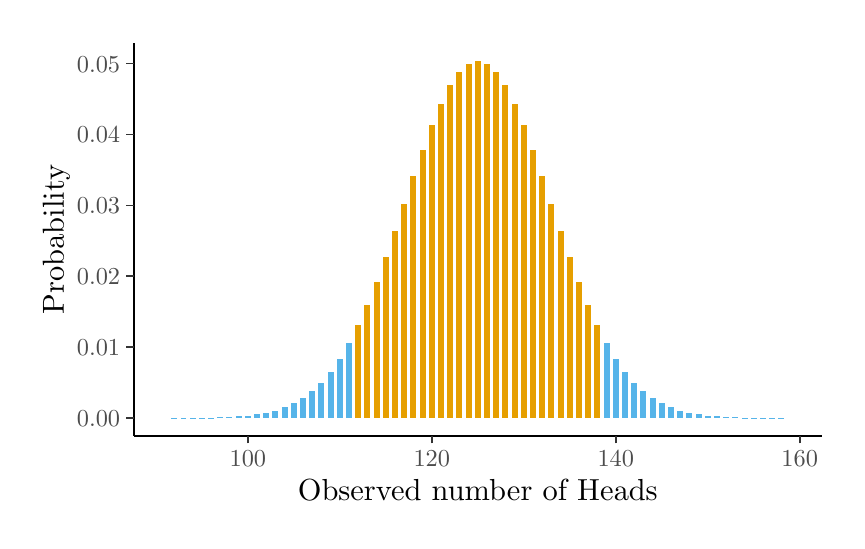
\begin{tikzpicture}[x=1pt,y=1pt]
\definecolor{fillColor}{RGB}{255,255,255}
\path[use as bounding box,fill=fillColor,fill opacity=0.00] (0,0) rectangle (292.45,178.21);
\begin{scope}
\path[clip] (  0.00,  0.00) rectangle (292.45,178.21);
\definecolor{drawColor}{RGB}{255,255,255}
\definecolor{fillColor}{RGB}{255,255,255}

\path[draw=drawColor,line width= 0.6pt,line join=round,line cap=round,fill=fillColor] (  0.00,  0.00) rectangle (292.45,178.21);
\end{scope}
\begin{scope}
\path[clip] ( 38.36, 30.72) rectangle (286.95,172.71);
\definecolor{fillColor}{RGB}{255,255,255}

\path[fill=fillColor] ( 38.36, 30.72) rectangle (286.95,172.71);
\definecolor{fillColor}{RGB}{86,180,233}

\path[fill=fillColor] ( 51.90, 37.18) rectangle ( 54.06, 37.20);

\path[fill=fillColor] ( 55.23, 37.18) rectangle ( 57.39, 37.21);

\path[fill=fillColor] ( 58.55, 37.18) rectangle ( 60.71, 37.23);

\path[fill=fillColor] ( 61.87, 37.18) rectangle ( 64.03, 37.27);

\path[fill=fillColor] ( 65.20, 37.18) rectangle ( 67.36, 37.33);

\path[fill=fillColor] ( 68.52, 37.18) rectangle ( 70.68, 37.42);

\path[fill=fillColor] ( 71.84, 37.18) rectangle ( 74.00, 37.55);

\path[fill=fillColor] ( 75.17, 37.18) rectangle ( 77.33, 37.75);

\path[fill=fillColor] ( 78.49, 37.18) rectangle ( 80.65, 38.04);

\path[fill=fillColor] ( 81.81, 37.18) rectangle ( 83.97, 38.45);

\path[fill=fillColor] ( 85.14, 37.18) rectangle ( 87.30, 39.04);

\path[fill=fillColor] ( 88.46, 37.18) rectangle ( 90.62, 39.85);

\path[fill=fillColor] ( 91.78, 37.18) rectangle ( 93.94, 40.96);

\path[fill=fillColor] ( 95.11, 37.18) rectangle ( 97.27, 42.44);

\path[fill=fillColor] ( 98.43, 37.18) rectangle (100.59, 44.37);

\path[fill=fillColor] (101.75, 37.18) rectangle (103.91, 46.86);

\path[fill=fillColor] (105.08, 37.18) rectangle (107.24, 49.99);

\path[fill=fillColor] (108.40, 37.18) rectangle (110.56, 53.87);

\path[fill=fillColor] (111.72, 37.18) rectangle (113.88, 58.58);

\path[fill=fillColor] (115.05, 37.18) rectangle (117.21, 64.17);
\definecolor{fillColor}{RGB}{230,159,0}

\path[fill=fillColor] (118.37, 37.18) rectangle (120.53, 70.67);

\path[fill=fillColor] (121.69, 37.18) rectangle (123.85, 78.08);

\path[fill=fillColor] (125.02, 37.18) rectangle (127.18, 86.34);

\path[fill=fillColor] (128.34, 37.18) rectangle (130.50, 95.31);

\path[fill=fillColor] (131.66, 37.18) rectangle (133.82,104.84);

\path[fill=fillColor] (134.99, 37.18) rectangle (137.15,114.67);

\path[fill=fillColor] (138.31, 37.18) rectangle (140.47,124.52);

\path[fill=fillColor] (141.63, 37.18) rectangle (143.79,134.06);

\path[fill=fillColor] (144.96, 37.18) rectangle (147.12,142.94);

\path[fill=fillColor] (148.28, 37.18) rectangle (150.44,150.80);

\path[fill=fillColor] (151.60, 37.18) rectangle (153.76,157.32);

\path[fill=fillColor] (154.93, 37.18) rectangle (157.09,162.21);

\path[fill=fillColor] (158.25, 37.18) rectangle (160.41,165.23);

\path[fill=fillColor] (161.57, 37.18) rectangle (163.73,166.26);

\path[fill=fillColor] (164.90, 37.18) rectangle (167.06,165.23);

\path[fill=fillColor] (168.22, 37.18) rectangle (170.38,162.21);

\path[fill=fillColor] (171.54, 37.18) rectangle (173.70,157.32);

\path[fill=fillColor] (174.87, 37.18) rectangle (177.03,150.80);

\path[fill=fillColor] (178.19, 37.18) rectangle (180.35,142.94);

\path[fill=fillColor] (181.51, 37.18) rectangle (183.68,134.06);

\path[fill=fillColor] (184.84, 37.18) rectangle (187.00,124.52);

\path[fill=fillColor] (188.16, 37.18) rectangle (190.32,114.67);

\path[fill=fillColor] (191.49, 37.18) rectangle (193.65,104.84);

\path[fill=fillColor] (194.81, 37.18) rectangle (196.97, 95.31);

\path[fill=fillColor] (198.13, 37.18) rectangle (200.29, 86.34);

\path[fill=fillColor] (201.46, 37.18) rectangle (203.62, 78.08);

\path[fill=fillColor] (204.78, 37.18) rectangle (206.94, 70.67);
\definecolor{fillColor}{RGB}{86,180,233}

\path[fill=fillColor] (208.10, 37.18) rectangle (210.26, 64.17);

\path[fill=fillColor] (211.43, 37.18) rectangle (213.59, 58.58);

\path[fill=fillColor] (214.75, 37.18) rectangle (216.91, 53.87);

\path[fill=fillColor] (218.07, 37.18) rectangle (220.23, 49.99);

\path[fill=fillColor] (221.40, 37.18) rectangle (223.56, 46.86);

\path[fill=fillColor] (224.72, 37.18) rectangle (226.88, 44.37);

\path[fill=fillColor] (228.04, 37.18) rectangle (230.20, 42.44);

\path[fill=fillColor] (231.37, 37.18) rectangle (233.53, 40.96);

\path[fill=fillColor] (234.69, 37.18) rectangle (236.85, 39.85);

\path[fill=fillColor] (238.01, 37.18) rectangle (240.17, 39.04);

\path[fill=fillColor] (241.34, 37.18) rectangle (243.50, 38.45);

\path[fill=fillColor] (244.66, 37.18) rectangle (246.82, 38.04);

\path[fill=fillColor] (247.98, 37.18) rectangle (250.14, 37.75);

\path[fill=fillColor] (251.31, 37.18) rectangle (253.47, 37.55);

\path[fill=fillColor] (254.63, 37.18) rectangle (256.79, 37.42);

\path[fill=fillColor] (257.95, 37.18) rectangle (260.11, 37.33);

\path[fill=fillColor] (261.28, 37.18) rectangle (263.44, 37.27);

\path[fill=fillColor] (264.60, 37.18) rectangle (266.76, 37.23);

\path[fill=fillColor] (267.92, 37.18) rectangle (270.08, 37.21);

\path[fill=fillColor] (271.25, 37.18) rectangle (273.41, 37.20);
\end{scope}
\begin{scope}
\path[clip] (  0.00,  0.00) rectangle (292.45,178.21);
\definecolor{drawColor}{RGB}{0,0,0}

\path[draw=drawColor,line width= 0.6pt,line join=round] ( 38.36, 30.72) --
	( 38.36,172.71);
\end{scope}
\begin{scope}
\path[clip] (  0.00,  0.00) rectangle (292.45,178.21);
\definecolor{drawColor}{gray}{0.30}

\node[text=drawColor,anchor=base east,inner sep=0pt, outer sep=0pt, scale=  0.88] at ( 33.41, 34.15) {0.00};

\node[text=drawColor,anchor=base east,inner sep=0pt, outer sep=0pt, scale=  0.88] at ( 33.41, 59.75) {0.01};

\node[text=drawColor,anchor=base east,inner sep=0pt, outer sep=0pt, scale=  0.88] at ( 33.41, 85.36) {0.02};

\node[text=drawColor,anchor=base east,inner sep=0pt, outer sep=0pt, scale=  0.88] at ( 33.41,110.96) {0.03};

\node[text=drawColor,anchor=base east,inner sep=0pt, outer sep=0pt, scale=  0.88] at ( 33.41,136.57) {0.04};

\node[text=drawColor,anchor=base east,inner sep=0pt, outer sep=0pt, scale=  0.88] at ( 33.41,162.17) {0.05};
\end{scope}
\begin{scope}
\path[clip] (  0.00,  0.00) rectangle (292.45,178.21);
\definecolor{drawColor}{gray}{0.20}

\path[draw=drawColor,line width= 0.6pt,line join=round] ( 35.61, 37.18) --
	( 38.36, 37.18);

\path[draw=drawColor,line width= 0.6pt,line join=round] ( 35.61, 62.78) --
	( 38.36, 62.78);

\path[draw=drawColor,line width= 0.6pt,line join=round] ( 35.61, 88.39) --
	( 38.36, 88.39);

\path[draw=drawColor,line width= 0.6pt,line join=round] ( 35.61,113.99) --
	( 38.36,113.99);

\path[draw=drawColor,line width= 0.6pt,line join=round] ( 35.61,139.60) --
	( 38.36,139.60);

\path[draw=drawColor,line width= 0.6pt,line join=round] ( 35.61,165.20) --
	( 38.36,165.20);
\end{scope}
\begin{scope}
\path[clip] (  0.00,  0.00) rectangle (292.45,178.21);
\definecolor{drawColor}{RGB}{0,0,0}

\path[draw=drawColor,line width= 0.6pt,line join=round] ( 38.36, 30.72) --
	(286.95, 30.72);
\end{scope}
\begin{scope}
\path[clip] (  0.00,  0.00) rectangle (292.45,178.21);
\definecolor{drawColor}{gray}{0.20}

\path[draw=drawColor,line width= 0.6pt,line join=round] ( 79.57, 27.97) --
	( 79.57, 30.72);

\path[draw=drawColor,line width= 0.6pt,line join=round] (146.04, 27.97) --
	(146.04, 30.72);

\path[draw=drawColor,line width= 0.6pt,line join=round] (212.51, 27.97) --
	(212.51, 30.72);

\path[draw=drawColor,line width= 0.6pt,line join=round] (278.97, 27.97) --
	(278.97, 30.72);
\end{scope}
\begin{scope}
\path[clip] (  0.00,  0.00) rectangle (292.45,178.21);
\definecolor{drawColor}{gray}{0.30}

\node[text=drawColor,anchor=base,inner sep=0pt, outer sep=0pt, scale=  0.88] at ( 79.57, 19.71) {100};

\node[text=drawColor,anchor=base,inner sep=0pt, outer sep=0pt, scale=  0.88] at (146.04, 19.71) {120};

\node[text=drawColor,anchor=base,inner sep=0pt, outer sep=0pt, scale=  0.88] at (212.51, 19.71) {140};

\node[text=drawColor,anchor=base,inner sep=0pt, outer sep=0pt, scale=  0.88] at (278.97, 19.71) {160};
\end{scope}
\begin{scope}
\path[clip] (  0.00,  0.00) rectangle (292.45,178.21);
\definecolor{drawColor}{RGB}{0,0,0}

\node[text=drawColor,anchor=base,inner sep=0pt, outer sep=0pt, scale=  1.10] at (162.65,  7.44) {Observed number of Heads};
\end{scope}
\begin{scope}
\path[clip] (  0.00,  0.00) rectangle (292.45,178.21);
\definecolor{drawColor}{RGB}{0,0,0}

\node[text=drawColor,rotate= 90.00,anchor=base,inner sep=0pt, outer sep=0pt, scale=  1.10] at ( 13.08,101.72) {Probability};
\end{scope}
\end{tikzpicture}

	{\small
	\begin{itemize}
	\item Areas shaded in blue are values \emph{as or more extreme} than $m=139$.
	\item For the interactive version: \url{https://lawsofthought.shinyapps.io/binomial_test/}.
	\end{itemize}
	}
\end{frame}

\begin{frame}
	\frametitle{Inference using the likelihood function}
		\begin{itemize}
			\item The likelihood function is a function over the parameter space, i.e. over $\theta$.
			\item It gives the probability\footnote{Strictly speaking, it gives the probability times an arbitrary positive constant $c$.}
				of the observed data, i.e. $m=139$ Heads in $n=250$ coin flips, for all possible values of $\theta$.
			\item As such, it tells us how well any possible value of $\theta$ predicts the observed data.
			\item We usually denote the likelihood function as follows:
				\[L(\theta\given\mathcal{D}) \propto \Prob{\mathcal{D}\given\theta},\]
				where $\mathcal{D}$ signifies the observed data, i.e. $\mathcal{D} = \{n=250, m=130\}$.
		\end{itemize}
\end{frame}

\begin{frame}
	\frametitle{The likelihood function versus sampling distribution}
		\begin{itemize}
			\item The sampling distribution is the binomial distribution:
				\[\Prob{m \given \theta,n} = \binom{n}{m} \theta^m (1-\theta)^{n-m}.\]
				This is always a function of $m$, with $\theta$ and $n$ fixed.
			\item The corresponding likelihood function treats the same function
		\[\Prob{m \given \theta,n} = \binom{n}{m} \theta^m (1-\theta)^{n-m},\] 
				as a function of $\theta$, but now with $m$ and $n$ fixed.
			\item As such, the binomial likelihood is 
				\[L(\theta\given\mathcal{D}) \propto \theta^m (1-\theta)^{n-m}.\]
\end{itemize}
\end{frame}



\begin{frame}
	\frametitle{Binomial likelihood}
	\framesubtitle{Given $n=250$ and $m=139$}.
	% Created by tikzDevice version 0.10.1 on 2017-07-05 01:07:16
% !TEX encoding = UTF-8 Unicode
\begin{tikzpicture}[x=1pt,y=1pt]
\definecolor{fillColor}{RGB}{255,255,255}
\path[use as bounding box,fill=fillColor,fill opacity=0.00] (0,0) rectangle (292.45,164.50);
\begin{scope}
\path[clip] (  0.00,  0.00) rectangle (292.45,164.50);
\definecolor{drawColor}{RGB}{255,255,255}
\definecolor{fillColor}{RGB}{255,255,255}

\path[draw=drawColor,line width= 0.6pt,line join=round,line cap=round,fill=fillColor] (  0.00,  0.00) rectangle (292.45,164.50);
\end{scope}
\begin{scope}
\path[clip] ( 21.55, 27.54) rectangle (286.95,159.00);
\definecolor{fillColor}{RGB}{255,255,255}

\path[fill=fillColor] ( 21.55, 27.54) rectangle (286.95,159.00);
\definecolor{drawColor}{RGB}{0,0,0}

\path[draw=drawColor,line width= 0.6pt,line join=round] ( 33.62, 33.52) --
	( 33.86, 33.52) --
	( 34.10, 33.52) --
	( 34.34, 33.52) --
	( 34.58, 33.52) --
	( 34.82, 33.52) --
	( 35.06, 33.52) --
	( 35.30, 33.52) --
	( 35.55, 33.52) --
	( 35.79, 33.52) --
	( 36.03, 33.52) --
	( 36.27, 33.52) --
	( 36.51, 33.52) --
	( 36.75, 33.52) --
	( 36.99, 33.52) --
	( 37.24, 33.52) --
	( 37.48, 33.52) --
	( 37.72, 33.52) --
	( 37.96, 33.52) --
	( 38.20, 33.52) --
	( 38.44, 33.52) --
	( 38.68, 33.52) --
	( 38.92, 33.52) --
	( 39.17, 33.52) --
	( 39.41, 33.52) --
	( 39.65, 33.52) --
	( 39.89, 33.52) --
	( 40.13, 33.52) --
	( 40.37, 33.52) --
	( 40.61, 33.52) --
	( 40.85, 33.52) --
	( 41.10, 33.52) --
	( 41.34, 33.52) --
	( 41.58, 33.52) --
	( 41.82, 33.52) --
	( 42.06, 33.52) --
	( 42.30, 33.52) --
	( 42.54, 33.52) --
	( 42.78, 33.52) --
	( 43.03, 33.52) --
	( 43.27, 33.52) --
	( 43.51, 33.52) --
	( 43.75, 33.52) --
	( 43.99, 33.52) --
	( 44.23, 33.52) --
	( 44.47, 33.52) --
	( 44.71, 33.52) --
	( 44.96, 33.52) --
	( 45.20, 33.52) --
	( 45.44, 33.52) --
	( 45.68, 33.52) --
	( 45.92, 33.52) --
	( 46.16, 33.52) --
	( 46.40, 33.52) --
	( 46.64, 33.52) --
	( 46.89, 33.52) --
	( 47.13, 33.52) --
	( 47.37, 33.52) --
	( 47.61, 33.52) --
	( 47.85, 33.52) --
	( 48.09, 33.52) --
	( 48.33, 33.52) --
	( 48.57, 33.52) --
	( 48.82, 33.52) --
	( 49.06, 33.52) --
	( 49.30, 33.52) --
	( 49.54, 33.52) --
	( 49.78, 33.52) --
	( 50.02, 33.52) --
	( 50.26, 33.52) --
	( 50.50, 33.52) --
	( 50.75, 33.52) --
	( 50.99, 33.52) --
	( 51.23, 33.52) --
	( 51.47, 33.52) --
	( 51.71, 33.52) --
	( 51.95, 33.52) --
	( 52.19, 33.52) --
	( 52.44, 33.52) --
	( 52.68, 33.52) --
	( 52.92, 33.52) --
	( 53.16, 33.52) --
	( 53.40, 33.52) --
	( 53.64, 33.52) --
	( 53.88, 33.52) --
	( 54.12, 33.52) --
	( 54.37, 33.52) --
	( 54.61, 33.52) --
	( 54.85, 33.52) --
	( 55.09, 33.52) --
	( 55.33, 33.52) --
	( 55.57, 33.52) --
	( 55.81, 33.52) --
	( 56.05, 33.52) --
	( 56.30, 33.52) --
	( 56.54, 33.52) --
	( 56.78, 33.52) --
	( 57.02, 33.52) --
	( 57.26, 33.52) --
	( 57.50, 33.52) --
	( 57.74, 33.52) --
	( 57.98, 33.52) --
	( 58.23, 33.52) --
	( 58.47, 33.52) --
	( 58.71, 33.52) --
	( 58.95, 33.52) --
	( 59.19, 33.52) --
	( 59.43, 33.52) --
	( 59.67, 33.52) --
	( 59.91, 33.52) --
	( 60.16, 33.52) --
	( 60.40, 33.52) --
	( 60.64, 33.52) --
	( 60.88, 33.52) --
	( 61.12, 33.52) --
	( 61.36, 33.52) --
	( 61.60, 33.52) --
	( 61.84, 33.52) --
	( 62.09, 33.52) --
	( 62.33, 33.52) --
	( 62.57, 33.52) --
	( 62.81, 33.52) --
	( 63.05, 33.52) --
	( 63.29, 33.52) --
	( 63.53, 33.52) --
	( 63.77, 33.52) --
	( 64.02, 33.52) --
	( 64.26, 33.52) --
	( 64.50, 33.52) --
	( 64.74, 33.52) --
	( 64.98, 33.52) --
	( 65.22, 33.52) --
	( 65.46, 33.52) --
	( 65.70, 33.52) --
	( 65.95, 33.52) --
	( 66.19, 33.52) --
	( 66.43, 33.52) --
	( 66.67, 33.52) --
	( 66.91, 33.52) --
	( 67.15, 33.52) --
	( 67.39, 33.52) --
	( 67.64, 33.52) --
	( 67.88, 33.52) --
	( 68.12, 33.52) --
	( 68.36, 33.52) --
	( 68.60, 33.52) --
	( 68.84, 33.52) --
	( 69.08, 33.52) --
	( 69.32, 33.52) --
	( 69.57, 33.52) --
	( 69.81, 33.52) --
	( 70.05, 33.52) --
	( 70.29, 33.52) --
	( 70.53, 33.52) --
	( 70.77, 33.52) --
	( 71.01, 33.52) --
	( 71.25, 33.52) --
	( 71.50, 33.52) --
	( 71.74, 33.52) --
	( 71.98, 33.52) --
	( 72.22, 33.52) --
	( 72.46, 33.52) --
	( 72.70, 33.52) --
	( 72.94, 33.52) --
	( 73.18, 33.52) --
	( 73.43, 33.52) --
	( 73.67, 33.52) --
	( 73.91, 33.52) --
	( 74.15, 33.52) --
	( 74.39, 33.52) --
	( 74.63, 33.52) --
	( 74.87, 33.52) --
	( 75.11, 33.52) --
	( 75.36, 33.52) --
	( 75.60, 33.52) --
	( 75.84, 33.52) --
	( 76.08, 33.52) --
	( 76.32, 33.52) --
	( 76.56, 33.52) --
	( 76.80, 33.52) --
	( 77.04, 33.52) --
	( 77.29, 33.52) --
	( 77.53, 33.52) --
	( 77.77, 33.52) --
	( 78.01, 33.52) --
	( 78.25, 33.52) --
	( 78.49, 33.52) --
	( 78.73, 33.52) --
	( 78.97, 33.52) --
	( 79.22, 33.52) --
	( 79.46, 33.52) --
	( 79.70, 33.52) --
	( 79.94, 33.52) --
	( 80.18, 33.52) --
	( 80.42, 33.52) --
	( 80.66, 33.52) --
	( 80.90, 33.52) --
	( 81.15, 33.52) --
	( 81.39, 33.52) --
	( 81.63, 33.52) --
	( 81.87, 33.52) --
	( 82.11, 33.52) --
	( 82.35, 33.52) --
	( 82.59, 33.52) --
	( 82.83, 33.52) --
	( 83.08, 33.52) --
	( 83.32, 33.52) --
	( 83.56, 33.52) --
	( 83.80, 33.52) --
	( 84.04, 33.52) --
	( 84.28, 33.52) --
	( 84.52, 33.52) --
	( 84.77, 33.52) --
	( 85.01, 33.52) --
	( 85.25, 33.52) --
	( 85.49, 33.52) --
	( 85.73, 33.52) --
	( 85.97, 33.52) --
	( 86.21, 33.52) --
	( 86.45, 33.52) --
	( 86.70, 33.52) --
	( 86.94, 33.52) --
	( 87.18, 33.52) --
	( 87.42, 33.52) --
	( 87.66, 33.52) --
	( 87.90, 33.52) --
	( 88.14, 33.52) --
	( 88.38, 33.52) --
	( 88.63, 33.52) --
	( 88.87, 33.52) --
	( 89.11, 33.52) --
	( 89.35, 33.52) --
	( 89.59, 33.52) --
	( 89.83, 33.52) --
	( 90.07, 33.52) --
	( 90.31, 33.52) --
	( 90.56, 33.52) --
	( 90.80, 33.52) --
	( 91.04, 33.52) --
	( 91.28, 33.52) --
	( 91.52, 33.52) --
	( 91.76, 33.52) --
	( 92.00, 33.52) --
	( 92.24, 33.52) --
	( 92.49, 33.52) --
	( 92.73, 33.52) --
	( 92.97, 33.52) --
	( 93.21, 33.52) --
	( 93.45, 33.52) --
	( 93.69, 33.52) --
	( 93.93, 33.52) --
	( 94.17, 33.52) --
	( 94.42, 33.52) --
	( 94.66, 33.52) --
	( 94.90, 33.52) --
	( 95.14, 33.52) --
	( 95.38, 33.52) --
	( 95.62, 33.52) --
	( 95.86, 33.52) --
	( 96.10, 33.52) --
	( 96.35, 33.52) --
	( 96.59, 33.52) --
	( 96.83, 33.52) --
	( 97.07, 33.52) --
	( 97.31, 33.52) --
	( 97.55, 33.52) --
	( 97.79, 33.52) --
	( 98.03, 33.52) --
	( 98.28, 33.52) --
	( 98.52, 33.52) --
	( 98.76, 33.52) --
	( 99.00, 33.52) --
	( 99.24, 33.52) --
	( 99.48, 33.52) --
	( 99.72, 33.52) --
	( 99.97, 33.52) --
	(100.21, 33.52) --
	(100.45, 33.52) --
	(100.69, 33.52) --
	(100.93, 33.52) --
	(101.17, 33.52) --
	(101.41, 33.52) --
	(101.65, 33.52) --
	(101.90, 33.52) --
	(102.14, 33.52) --
	(102.38, 33.52) --
	(102.62, 33.52) --
	(102.86, 33.52) --
	(103.10, 33.52) --
	(103.34, 33.52) --
	(103.58, 33.52) --
	(103.83, 33.52) --
	(104.07, 33.52) --
	(104.31, 33.52) --
	(104.55, 33.52) --
	(104.79, 33.52) --
	(105.03, 33.52) --
	(105.27, 33.52) --
	(105.51, 33.52) --
	(105.76, 33.52) --
	(106.00, 33.52) --
	(106.24, 33.52) --
	(106.48, 33.52) --
	(106.72, 33.52) --
	(106.96, 33.52) --
	(107.20, 33.52) --
	(107.44, 33.52) --
	(107.69, 33.52) --
	(107.93, 33.52) --
	(108.17, 33.52) --
	(108.41, 33.52) --
	(108.65, 33.52) --
	(108.89, 33.52) --
	(109.13, 33.52) --
	(109.37, 33.52) --
	(109.62, 33.52) --
	(109.86, 33.52) --
	(110.10, 33.52) --
	(110.34, 33.52) --
	(110.58, 33.52) --
	(110.82, 33.52) --
	(111.06, 33.52) --
	(111.30, 33.52) --
	(111.55, 33.52) --
	(111.79, 33.52) --
	(112.03, 33.52) --
	(112.27, 33.52) --
	(112.51, 33.52) --
	(112.75, 33.52) --
	(112.99, 33.52) --
	(113.23, 33.52) --
	(113.48, 33.52) --
	(113.72, 33.52) --
	(113.96, 33.52) --
	(114.20, 33.52) --
	(114.44, 33.52) --
	(114.68, 33.52) --
	(114.92, 33.52) --
	(115.17, 33.52) --
	(115.41, 33.52) --
	(115.65, 33.52) --
	(115.89, 33.52) --
	(116.13, 33.52) --
	(116.37, 33.52) --
	(116.61, 33.52) --
	(116.85, 33.52) --
	(117.10, 33.52) --
	(117.34, 33.52) --
	(117.58, 33.52) --
	(117.82, 33.52) --
	(118.06, 33.52) --
	(118.30, 33.52) --
	(118.54, 33.52) --
	(118.78, 33.52) --
	(119.03, 33.52) --
	(119.27, 33.52) --
	(119.51, 33.52) --
	(119.75, 33.52) --
	(119.99, 33.52) --
	(120.23, 33.52) --
	(120.47, 33.52) --
	(120.71, 33.52) --
	(120.96, 33.52) --
	(121.20, 33.52) --
	(121.44, 33.52) --
	(121.68, 33.52) --
	(121.92, 33.52) --
	(122.16, 33.52) --
	(122.40, 33.52) --
	(122.64, 33.52) --
	(122.89, 33.52) --
	(123.13, 33.52) --
	(123.37, 33.52) --
	(123.61, 33.52) --
	(123.85, 33.52) --
	(124.09, 33.52) --
	(124.33, 33.52) --
	(124.57, 33.52) --
	(124.82, 33.52) --
	(125.06, 33.52) --
	(125.30, 33.52) --
	(125.54, 33.52) --
	(125.78, 33.52) --
	(126.02, 33.52) --
	(126.26, 33.52) --
	(126.50, 33.52) --
	(126.75, 33.52) --
	(126.99, 33.52) --
	(127.23, 33.52) --
	(127.47, 33.52) --
	(127.71, 33.52) --
	(127.95, 33.52) --
	(128.19, 33.52) --
	(128.43, 33.52) --
	(128.68, 33.52) --
	(128.92, 33.52) --
	(129.16, 33.52) --
	(129.40, 33.52) --
	(129.64, 33.52) --
	(129.88, 33.52) --
	(130.12, 33.52) --
	(130.37, 33.52) --
	(130.61, 33.52) --
	(130.85, 33.52) --
	(131.09, 33.52) --
	(131.33, 33.52) --
	(131.57, 33.52) --
	(131.81, 33.52) --
	(132.05, 33.52) --
	(132.30, 33.52) --
	(132.54, 33.52) --
	(132.78, 33.52) --
	(133.02, 33.52) --
	(133.26, 33.52) --
	(133.50, 33.52) --
	(133.74, 33.52) --
	(133.98, 33.52) --
	(134.23, 33.52) --
	(134.47, 33.52) --
	(134.71, 33.53) --
	(134.95, 33.53) --
	(135.19, 33.53) --
	(135.43, 33.53) --
	(135.67, 33.53) --
	(135.91, 33.53) --
	(136.16, 33.54) --
	(136.40, 33.54) --
	(136.64, 33.54) --
	(136.88, 33.55) --
	(137.12, 33.55) --
	(137.36, 33.56) --
	(137.60, 33.56) --
	(137.84, 33.57) --
	(138.09, 33.58) --
	(138.33, 33.58) --
	(138.57, 33.59) --
	(138.81, 33.60) --
	(139.05, 33.61) --
	(139.29, 33.63) --
	(139.53, 33.64) --
	(139.77, 33.65) --
	(140.02, 33.67) --
	(140.26, 33.69) --
	(140.50, 33.71) --
	(140.74, 33.74) --
	(140.98, 33.76) --
	(141.22, 33.79) --
	(141.46, 33.82) --
	(141.70, 33.86) --
	(141.95, 33.90) --
	(142.19, 33.94) --
	(142.43, 33.99) --
	(142.67, 34.04) --
	(142.91, 34.10) --
	(143.15, 34.16) --
	(143.39, 34.23) --
	(143.63, 34.31) --
	(143.88, 34.39) --
	(144.12, 34.49) --
	(144.36, 34.59) --
	(144.60, 34.70) --
	(144.84, 34.81) --
	(145.08, 34.94) --
	(145.32, 35.08) --
	(145.57, 35.24) --
	(145.81, 35.40) --
	(146.05, 35.58) --
	(146.29, 35.78) --
	(146.53, 35.99) --
	(146.77, 36.21) --
	(147.01, 36.46) --
	(147.25, 36.72) --
	(147.50, 37.01) --
	(147.74, 37.31) --
	(147.98, 37.64) --
	(148.22, 37.99) --
	(148.46, 38.36) --
	(148.70, 38.77) --
	(148.94, 39.20) --
	(149.18, 39.66) --
	(149.43, 40.14) --
	(149.67, 40.67) --
	(149.91, 41.22) --
	(150.15, 41.81) --
	(150.39, 42.43) --
	(150.63, 43.09) --
	(150.87, 43.79) --
	(151.11, 44.53) --
	(151.36, 45.31) --
	(151.60, 46.14) --
	(151.84, 47.01) --
	(152.08, 47.92) --
	(152.32, 48.88) --
	(152.56, 49.89) --
	(152.80, 50.94) --
	(153.04, 52.05) --
	(153.29, 53.21) --
	(153.53, 54.41) --
	(153.77, 55.67) --
	(154.01, 56.98) --
	(154.25, 58.35) --
	(154.49, 59.76) --
	(154.73, 61.23) --
	(154.97, 62.76) --
	(155.22, 64.33) --
	(155.46, 65.96) --
	(155.70, 67.64) --
	(155.94, 69.38) --
	(156.18, 71.16) --
	(156.42, 72.99) --
	(156.66, 74.87) --
	(156.90, 76.80) --
	(157.15, 78.77) --
	(157.39, 80.78) --
	(157.63, 82.83) --
	(157.87, 84.93) --
	(158.11, 87.05) --
	(158.35, 89.21) --
	(158.59, 91.40) --
	(158.83, 93.62) --
	(159.08, 95.85) --
	(159.32, 98.11) --
	(159.56,100.38) --
	(159.80,102.66) --
	(160.04,104.95) --
	(160.28,107.24) --
	(160.52,109.53) --
	(160.76,111.82) --
	(161.01,114.09) --
	(161.25,116.34) --
	(161.49,118.57) --
	(161.73,120.78) --
	(161.97,122.95) --
	(162.21,125.09) --
	(162.45,127.18) --
	(162.70,129.23) --
	(162.94,131.22) --
	(163.18,133.15) --
	(163.42,135.02) --
	(163.66,136.83) --
	(163.90,138.56) --
	(164.14,140.21) --
	(164.38,141.78) --
	(164.63,143.26) --
	(164.87,144.65) --
	(165.11,145.95) --
	(165.35,147.14) --
	(165.59,148.24) --
	(165.83,149.22) --
	(166.07,150.10) --
	(166.31,150.87) --
	(166.56,151.53) --
	(166.80,152.06) --
	(167.04,152.48) --
	(167.28,152.79) --
	(167.52,152.97) --
	(167.76,153.03) --
	(168.00,152.97) --
	(168.24,152.79) --
	(168.49,152.48) --
	(168.73,152.06) --
	(168.97,151.52) --
	(169.21,150.86) --
	(169.45,150.09) --
	(169.69,149.21) --
	(169.93,148.21) --
	(170.17,147.11) --
	(170.42,145.90) --
	(170.66,144.59) --
	(170.90,143.19) --
	(171.14,141.69) --
	(171.38,140.10) --
	(171.62,138.42) --
	(171.86,136.67) --
	(172.10,134.84) --
	(172.35,132.94) --
	(172.59,130.98) --
	(172.83,128.95) --
	(173.07,126.87) --
	(173.31,124.75) --
	(173.55,122.57) --
	(173.79,120.36) --
	(174.03,118.11) --
	(174.28,115.84) --
	(174.52,113.55) --
	(174.76,111.23) --
	(175.00,108.91) --
	(175.24,106.57) --
	(175.48,104.24) --
	(175.72,101.90) --
	(175.96, 99.58) --
	(176.21, 97.26) --
	(176.45, 94.96) --
	(176.69, 92.68) --
	(176.93, 90.43) --
	(177.17, 88.20) --
	(177.41, 86.00) --
	(177.65, 83.84) --
	(177.90, 81.72) --
	(178.14, 79.63) --
	(178.38, 77.59) --
	(178.62, 75.59) --
	(178.86, 73.64) --
	(179.10, 71.74) --
	(179.34, 69.89) --
	(179.58, 68.09) --
	(179.83, 66.35) --
	(180.07, 64.65) --
	(180.31, 63.02) --
	(180.55, 61.44) --
	(180.79, 59.91) --
	(181.03, 58.44) --
	(181.27, 57.03) --
	(181.51, 55.67) --
	(181.76, 54.37) --
	(182.00, 53.12) --
	(182.24, 51.92) --
	(182.48, 50.78) --
	(182.72, 49.69) --
	(182.96, 48.66) --
	(183.20, 47.67) --
	(183.44, 46.73) --
	(183.69, 45.85) --
	(183.93, 45.00) --
	(184.17, 44.21) --
	(184.41, 43.45) --
	(184.65, 42.74) --
	(184.89, 42.07) --
	(185.13, 41.44) --
	(185.37, 40.85) --
	(185.62, 40.30) --
	(185.86, 39.78) --
	(186.10, 39.29) --
	(186.34, 38.83) --
	(186.58, 38.41) --
	(186.82, 38.01) --
	(187.06, 37.64) --
	(187.30, 37.30) --
	(187.55, 36.98) --
	(187.79, 36.68) --
	(188.03, 36.41) --
	(188.27, 36.15) --
	(188.51, 35.92) --
	(188.75, 35.70) --
	(188.99, 35.50) --
	(189.23, 35.32) --
	(189.48, 35.15) --
	(189.72, 35.00) --
	(189.96, 34.86) --
	(190.20, 34.73) --
	(190.44, 34.61) --
	(190.68, 34.50) --
	(190.92, 34.40) --
	(191.16, 34.31) --
	(191.41, 34.23) --
	(191.65, 34.16) --
	(191.89, 34.09) --
	(192.13, 34.03) --
	(192.37, 33.98) --
	(192.61, 33.93) --
	(192.85, 33.88) --
	(193.10, 33.84) --
	(193.34, 33.81) --
	(193.58, 33.77) --
	(193.82, 33.74) --
	(194.06, 33.72) --
	(194.30, 33.69) --
	(194.54, 33.67) --
	(194.78, 33.66) --
	(195.03, 33.64) --
	(195.27, 33.62) --
	(195.51, 33.61) --
	(195.75, 33.60) --
	(195.99, 33.59) --
	(196.23, 33.58) --
	(196.47, 33.57) --
	(196.71, 33.56) --
	(196.96, 33.56) --
	(197.20, 33.55) --
	(197.44, 33.55) --
	(197.68, 33.54) --
	(197.92, 33.54) --
	(198.16, 33.54) --
	(198.40, 33.53) --
	(198.64, 33.53) --
	(198.89, 33.53) --
	(199.13, 33.53) --
	(199.37, 33.53) --
	(199.61, 33.52) --
	(199.85, 33.52) --
	(200.09, 33.52) --
	(200.33, 33.52) --
	(200.57, 33.52) --
	(200.82, 33.52) --
	(201.06, 33.52) --
	(201.30, 33.52) --
	(201.54, 33.52) --
	(201.78, 33.52) --
	(202.02, 33.52) --
	(202.26, 33.52) --
	(202.50, 33.52) --
	(202.75, 33.52) --
	(202.99, 33.52) --
	(203.23, 33.52) --
	(203.47, 33.52) --
	(203.71, 33.52) --
	(203.95, 33.52) --
	(204.19, 33.52) --
	(204.43, 33.52) --
	(204.68, 33.52) --
	(204.92, 33.52) --
	(205.16, 33.52) --
	(205.40, 33.52) --
	(205.64, 33.52) --
	(205.88, 33.52) --
	(206.12, 33.52) --
	(206.36, 33.52) --
	(206.61, 33.52) --
	(206.85, 33.52) --
	(207.09, 33.52) --
	(207.33, 33.52) --
	(207.57, 33.52) --
	(207.81, 33.52) --
	(208.05, 33.52) --
	(208.30, 33.52) --
	(208.54, 33.52) --
	(208.78, 33.52) --
	(209.02, 33.52) --
	(209.26, 33.52) --
	(209.50, 33.52) --
	(209.74, 33.52) --
	(209.98, 33.52) --
	(210.23, 33.52) --
	(210.47, 33.52) --
	(210.71, 33.52) --
	(210.95, 33.52) --
	(211.19, 33.52) --
	(211.43, 33.52) --
	(211.67, 33.52) --
	(211.91, 33.52) --
	(212.16, 33.52) --
	(212.40, 33.52) --
	(212.64, 33.52) --
	(212.88, 33.52) --
	(213.12, 33.52) --
	(213.36, 33.52) --
	(213.60, 33.52) --
	(213.84, 33.52) --
	(214.09, 33.52) --
	(214.33, 33.52) --
	(214.57, 33.52) --
	(214.81, 33.52) --
	(215.05, 33.52) --
	(215.29, 33.52) --
	(215.53, 33.52) --
	(215.77, 33.52) --
	(216.02, 33.52) --
	(216.26, 33.52) --
	(216.50, 33.52) --
	(216.74, 33.52) --
	(216.98, 33.52) --
	(217.22, 33.52) --
	(217.46, 33.52) --
	(217.70, 33.52) --
	(217.95, 33.52) --
	(218.19, 33.52) --
	(218.43, 33.52) --
	(218.67, 33.52) --
	(218.91, 33.52) --
	(219.15, 33.52) --
	(219.39, 33.52) --
	(219.63, 33.52) --
	(219.88, 33.52) --
	(220.12, 33.52) --
	(220.36, 33.52) --
	(220.60, 33.52) --
	(220.84, 33.52) --
	(221.08, 33.52) --
	(221.32, 33.52) --
	(221.56, 33.52) --
	(221.81, 33.52) --
	(222.05, 33.52) --
	(222.29, 33.52) --
	(222.53, 33.52) --
	(222.77, 33.52) --
	(223.01, 33.52) --
	(223.25, 33.52) --
	(223.50, 33.52) --
	(223.74, 33.52) --
	(223.98, 33.52) --
	(224.22, 33.52) --
	(224.46, 33.52) --
	(224.70, 33.52) --
	(224.94, 33.52) --
	(225.18, 33.52) --
	(225.43, 33.52) --
	(225.67, 33.52) --
	(225.91, 33.52) --
	(226.15, 33.52) --
	(226.39, 33.52) --
	(226.63, 33.52) --
	(226.87, 33.52) --
	(227.11, 33.52) --
	(227.36, 33.52) --
	(227.60, 33.52) --
	(227.84, 33.52) --
	(228.08, 33.52) --
	(228.32, 33.52) --
	(228.56, 33.52) --
	(228.80, 33.52) --
	(229.04, 33.52) --
	(229.29, 33.52) --
	(229.53, 33.52) --
	(229.77, 33.52) --
	(230.01, 33.52) --
	(230.25, 33.52) --
	(230.49, 33.52) --
	(230.73, 33.52) --
	(230.97, 33.52) --
	(231.22, 33.52) --
	(231.46, 33.52) --
	(231.70, 33.52) --
	(231.94, 33.52) --
	(232.18, 33.52) --
	(232.42, 33.52) --
	(232.66, 33.52) --
	(232.90, 33.52) --
	(233.15, 33.52) --
	(233.39, 33.52) --
	(233.63, 33.52) --
	(233.87, 33.52) --
	(234.11, 33.52) --
	(234.35, 33.52) --
	(234.59, 33.52) --
	(234.83, 33.52) --
	(235.08, 33.52) --
	(235.32, 33.52) --
	(235.56, 33.52) --
	(235.80, 33.52) --
	(236.04, 33.52) --
	(236.28, 33.52) --
	(236.52, 33.52) --
	(236.76, 33.52) --
	(237.01, 33.52) --
	(237.25, 33.52) --
	(237.49, 33.52) --
	(237.73, 33.52) --
	(237.97, 33.52) --
	(238.21, 33.52) --
	(238.45, 33.52) --
	(238.70, 33.52) --
	(238.94, 33.52) --
	(239.18, 33.52) --
	(239.42, 33.52) --
	(239.66, 33.52) --
	(239.90, 33.52) --
	(240.14, 33.52) --
	(240.38, 33.52) --
	(240.63, 33.52) --
	(240.87, 33.52) --
	(241.11, 33.52) --
	(241.35, 33.52) --
	(241.59, 33.52) --
	(241.83, 33.52) --
	(242.07, 33.52) --
	(242.31, 33.52) --
	(242.56, 33.52) --
	(242.80, 33.52) --
	(243.04, 33.52) --
	(243.28, 33.52) --
	(243.52, 33.52) --
	(243.76, 33.52) --
	(244.00, 33.52) --
	(244.24, 33.52) --
	(244.49, 33.52) --
	(244.73, 33.52) --
	(244.97, 33.52) --
	(245.21, 33.52) --
	(245.45, 33.52) --
	(245.69, 33.52) --
	(245.93, 33.52) --
	(246.17, 33.52) --
	(246.42, 33.52) --
	(246.66, 33.52) --
	(246.90, 33.52) --
	(247.14, 33.52) --
	(247.38, 33.52) --
	(247.62, 33.52) --
	(247.86, 33.52) --
	(248.10, 33.52) --
	(248.35, 33.52) --
	(248.59, 33.52) --
	(248.83, 33.52) --
	(249.07, 33.52) --
	(249.31, 33.52) --
	(249.55, 33.52) --
	(249.79, 33.52) --
	(250.03, 33.52) --
	(250.28, 33.52) --
	(250.52, 33.52) --
	(250.76, 33.52) --
	(251.00, 33.52) --
	(251.24, 33.52) --
	(251.48, 33.52) --
	(251.72, 33.52) --
	(251.96, 33.52) --
	(252.21, 33.52) --
	(252.45, 33.52) --
	(252.69, 33.52) --
	(252.93, 33.52) --
	(253.17, 33.52) --
	(253.41, 33.52) --
	(253.65, 33.52) --
	(253.89, 33.52) --
	(254.14, 33.52) --
	(254.38, 33.52) --
	(254.62, 33.52) --
	(254.86, 33.52) --
	(255.10, 33.52) --
	(255.34, 33.52) --
	(255.58, 33.52) --
	(255.83, 33.52) --
	(256.07, 33.52) --
	(256.31, 33.52) --
	(256.55, 33.52) --
	(256.79, 33.52) --
	(257.03, 33.52) --
	(257.27, 33.52) --
	(257.51, 33.52) --
	(257.76, 33.52) --
	(258.00, 33.52) --
	(258.24, 33.52) --
	(258.48, 33.52) --
	(258.72, 33.52) --
	(258.96, 33.52) --
	(259.20, 33.52) --
	(259.44, 33.52) --
	(259.69, 33.52) --
	(259.93, 33.52) --
	(260.17, 33.52) --
	(260.41, 33.52) --
	(260.65, 33.52) --
	(260.89, 33.52) --
	(261.13, 33.52) --
	(261.37, 33.52) --
	(261.62, 33.52) --
	(261.86, 33.52) --
	(262.10, 33.52) --
	(262.34, 33.52) --
	(262.58, 33.52) --
	(262.82, 33.52) --
	(263.06, 33.52) --
	(263.30, 33.52) --
	(263.55, 33.52) --
	(263.79, 33.52) --
	(264.03, 33.52) --
	(264.27, 33.52) --
	(264.51, 33.52) --
	(264.75, 33.52) --
	(264.99, 33.52) --
	(265.23, 33.52) --
	(265.48, 33.52) --
	(265.72, 33.52) --
	(265.96, 33.52) --
	(266.20, 33.52) --
	(266.44, 33.52) --
	(266.68, 33.52) --
	(266.92, 33.52) --
	(267.16, 33.52) --
	(267.41, 33.52) --
	(267.65, 33.52) --
	(267.89, 33.52) --
	(268.13, 33.52) --
	(268.37, 33.52) --
	(268.61, 33.52) --
	(268.85, 33.52) --
	(269.09, 33.52) --
	(269.34, 33.52) --
	(269.58, 33.52) --
	(269.82, 33.52) --
	(270.06, 33.52) --
	(270.30, 33.52) --
	(270.54, 33.52) --
	(270.78, 33.52) --
	(271.03, 33.52) --
	(271.27, 33.52) --
	(271.51, 33.52) --
	(271.75, 33.52) --
	(271.99, 33.52) --
	(272.23, 33.52) --
	(272.47, 33.52) --
	(272.71, 33.52) --
	(272.96, 33.52) --
	(273.20, 33.52) --
	(273.44, 33.52) --
	(273.68, 33.52) --
	(273.92, 33.52) --
	(274.16, 33.52) --
	(274.40, 33.52) --
	(274.64, 33.52) --
	(274.89, 33.52);
\definecolor{drawColor}{RGB}{255,0,0}

\path[draw=drawColor,line width= 0.6pt,line join=round] (155.01, 63.00) -- (180.31, 63.00);

\path[draw=drawColor,line width= 0.6pt,line join=round] (155.01, 63.00) -- (180.31, 63.00);

\path[draw=drawColor,line width= 0.6pt,line join=round] (155.01, 63.00) -- (180.31, 63.00);

\path[draw=drawColor,line width= 0.6pt,line join=round] (155.01, 63.00) -- (180.31, 63.00);

\path[draw=drawColor,line width= 0.6pt,line join=round] (155.01, 63.00) -- (180.31, 63.00);

\path[draw=drawColor,line width= 0.6pt,line join=round] (155.01, 63.00) -- (180.31, 63.00);

\path[draw=drawColor,line width= 0.6pt,line join=round] (155.01, 63.00) -- (180.31, 63.00);

\path[draw=drawColor,line width= 0.6pt,line join=round] (155.01, 63.00) -- (180.31, 63.00);

\path[draw=drawColor,line width= 0.6pt,line join=round] (155.01, 63.00) -- (180.31, 63.00);

\path[draw=drawColor,line width= 0.6pt,line join=round] (155.01, 63.00) -- (180.31, 63.00);

\path[draw=drawColor,line width= 0.6pt,line join=round] (155.01, 63.00) -- (180.31, 63.00);

\path[draw=drawColor,line width= 0.6pt,line join=round] (155.01, 63.00) -- (180.31, 63.00);

\path[draw=drawColor,line width= 0.6pt,line join=round] (155.01, 63.00) -- (180.31, 63.00);

\path[draw=drawColor,line width= 0.6pt,line join=round] (155.01, 63.00) -- (180.31, 63.00);

\path[draw=drawColor,line width= 0.6pt,line join=round] (155.01, 63.00) -- (180.31, 63.00);

\path[draw=drawColor,line width= 0.6pt,line join=round] (155.01, 63.00) -- (180.31, 63.00);

\path[draw=drawColor,line width= 0.6pt,line join=round] (155.01, 63.00) -- (180.31, 63.00);

\path[draw=drawColor,line width= 0.6pt,line join=round] (155.01, 63.00) -- (180.31, 63.00);

\path[draw=drawColor,line width= 0.6pt,line join=round] (155.01, 63.00) -- (180.31, 63.00);

\path[draw=drawColor,line width= 0.6pt,line join=round] (155.01, 63.00) -- (180.31, 63.00);

\path[draw=drawColor,line width= 0.6pt,line join=round] (155.01, 63.00) -- (180.31, 63.00);

\path[draw=drawColor,line width= 0.6pt,line join=round] (155.01, 63.00) -- (180.31, 63.00);

\path[draw=drawColor,line width= 0.6pt,line join=round] (155.01, 63.00) -- (180.31, 63.00);

\path[draw=drawColor,line width= 0.6pt,line join=round] (155.01, 63.00) -- (180.31, 63.00);

\path[draw=drawColor,line width= 0.6pt,line join=round] (155.01, 63.00) -- (180.31, 63.00);

\path[draw=drawColor,line width= 0.6pt,line join=round] (155.01, 63.00) -- (180.31, 63.00);

\path[draw=drawColor,line width= 0.6pt,line join=round] (155.01, 63.00) -- (180.31, 63.00);

\path[draw=drawColor,line width= 0.6pt,line join=round] (155.01, 63.00) -- (180.31, 63.00);

\path[draw=drawColor,line width= 0.6pt,line join=round] (155.01, 63.00) -- (180.31, 63.00);

\path[draw=drawColor,line width= 0.6pt,line join=round] (155.01, 63.00) -- (180.31, 63.00);

\path[draw=drawColor,line width= 0.6pt,line join=round] (155.01, 63.00) -- (180.31, 63.00);

\path[draw=drawColor,line width= 0.6pt,line join=round] (155.01, 63.00) -- (180.31, 63.00);

\path[draw=drawColor,line width= 0.6pt,line join=round] (155.01, 63.00) -- (180.31, 63.00);

\path[draw=drawColor,line width= 0.6pt,line join=round] (155.01, 63.00) -- (180.31, 63.00);

\path[draw=drawColor,line width= 0.6pt,line join=round] (155.01, 63.00) -- (180.31, 63.00);

\path[draw=drawColor,line width= 0.6pt,line join=round] (155.01, 63.00) -- (180.31, 63.00);

\path[draw=drawColor,line width= 0.6pt,line join=round] (155.01, 63.00) -- (180.31, 63.00);

\path[draw=drawColor,line width= 0.6pt,line join=round] (155.01, 63.00) -- (180.31, 63.00);

\path[draw=drawColor,line width= 0.6pt,line join=round] (155.01, 63.00) -- (180.31, 63.00);

\path[draw=drawColor,line width= 0.6pt,line join=round] (155.01, 63.00) -- (180.31, 63.00);

\path[draw=drawColor,line width= 0.6pt,line join=round] (155.01, 63.00) -- (180.31, 63.00);

\path[draw=drawColor,line width= 0.6pt,line join=round] (155.01, 63.00) -- (180.31, 63.00);

\path[draw=drawColor,line width= 0.6pt,line join=round] (155.01, 63.00) -- (180.31, 63.00);

\path[draw=drawColor,line width= 0.6pt,line join=round] (155.01, 63.00) -- (180.31, 63.00);

\path[draw=drawColor,line width= 0.6pt,line join=round] (155.01, 63.00) -- (180.31, 63.00);

\path[draw=drawColor,line width= 0.6pt,line join=round] (155.01, 63.00) -- (180.31, 63.00);

\path[draw=drawColor,line width= 0.6pt,line join=round] (155.01, 63.00) -- (180.31, 63.00);

\path[draw=drawColor,line width= 0.6pt,line join=round] (155.01, 63.00) -- (180.31, 63.00);

\path[draw=drawColor,line width= 0.6pt,line join=round] (155.01, 63.00) -- (180.31, 63.00);

\path[draw=drawColor,line width= 0.6pt,line join=round] (155.01, 63.00) -- (180.31, 63.00);

\path[draw=drawColor,line width= 0.6pt,line join=round] (155.01, 63.00) -- (180.31, 63.00);

\path[draw=drawColor,line width= 0.6pt,line join=round] (155.01, 63.00) -- (180.31, 63.00);

\path[draw=drawColor,line width= 0.6pt,line join=round] (155.01, 63.00) -- (180.31, 63.00);

\path[draw=drawColor,line width= 0.6pt,line join=round] (155.01, 63.00) -- (180.31, 63.00);

\path[draw=drawColor,line width= 0.6pt,line join=round] (155.01, 63.00) -- (180.31, 63.00);

\path[draw=drawColor,line width= 0.6pt,line join=round] (155.01, 63.00) -- (180.31, 63.00);

\path[draw=drawColor,line width= 0.6pt,line join=round] (155.01, 63.00) -- (180.31, 63.00);

\path[draw=drawColor,line width= 0.6pt,line join=round] (155.01, 63.00) -- (180.31, 63.00);

\path[draw=drawColor,line width= 0.6pt,line join=round] (155.01, 63.00) -- (180.31, 63.00);

\path[draw=drawColor,line width= 0.6pt,line join=round] (155.01, 63.00) -- (180.31, 63.00);

\path[draw=drawColor,line width= 0.6pt,line join=round] (155.01, 63.00) -- (180.31, 63.00);

\path[draw=drawColor,line width= 0.6pt,line join=round] (155.01, 63.00) -- (180.31, 63.00);

\path[draw=drawColor,line width= 0.6pt,line join=round] (155.01, 63.00) -- (180.31, 63.00);

\path[draw=drawColor,line width= 0.6pt,line join=round] (155.01, 63.00) -- (180.31, 63.00);

\path[draw=drawColor,line width= 0.6pt,line join=round] (155.01, 63.00) -- (180.31, 63.00);

\path[draw=drawColor,line width= 0.6pt,line join=round] (155.01, 63.00) -- (180.31, 63.00);

\path[draw=drawColor,line width= 0.6pt,line join=round] (155.01, 63.00) -- (180.31, 63.00);

\path[draw=drawColor,line width= 0.6pt,line join=round] (155.01, 63.00) -- (180.31, 63.00);

\path[draw=drawColor,line width= 0.6pt,line join=round] (155.01, 63.00) -- (180.31, 63.00);

\path[draw=drawColor,line width= 0.6pt,line join=round] (155.01, 63.00) -- (180.31, 63.00);

\path[draw=drawColor,line width= 0.6pt,line join=round] (155.01, 63.00) -- (180.31, 63.00);

\path[draw=drawColor,line width= 0.6pt,line join=round] (155.01, 63.00) -- (180.31, 63.00);

\path[draw=drawColor,line width= 0.6pt,line join=round] (155.01, 63.00) -- (180.31, 63.00);

\path[draw=drawColor,line width= 0.6pt,line join=round] (155.01, 63.00) -- (180.31, 63.00);

\path[draw=drawColor,line width= 0.6pt,line join=round] (155.01, 63.00) -- (180.31, 63.00);

\path[draw=drawColor,line width= 0.6pt,line join=round] (155.01, 63.00) -- (180.31, 63.00);

\path[draw=drawColor,line width= 0.6pt,line join=round] (155.01, 63.00) -- (180.31, 63.00);

\path[draw=drawColor,line width= 0.6pt,line join=round] (155.01, 63.00) -- (180.31, 63.00);

\path[draw=drawColor,line width= 0.6pt,line join=round] (155.01, 63.00) -- (180.31, 63.00);

\path[draw=drawColor,line width= 0.6pt,line join=round] (155.01, 63.00) -- (180.31, 63.00);

\path[draw=drawColor,line width= 0.6pt,line join=round] (155.01, 63.00) -- (180.31, 63.00);

\path[draw=drawColor,line width= 0.6pt,line join=round] (155.01, 63.00) -- (180.31, 63.00);

\path[draw=drawColor,line width= 0.6pt,line join=round] (155.01, 63.00) -- (180.31, 63.00);

\path[draw=drawColor,line width= 0.6pt,line join=round] (155.01, 63.00) -- (180.31, 63.00);

\path[draw=drawColor,line width= 0.6pt,line join=round] (155.01, 63.00) -- (180.31, 63.00);

\path[draw=drawColor,line width= 0.6pt,line join=round] (155.01, 63.00) -- (180.31, 63.00);

\path[draw=drawColor,line width= 0.6pt,line join=round] (155.01, 63.00) -- (180.31, 63.00);

\path[draw=drawColor,line width= 0.6pt,line join=round] (155.01, 63.00) -- (180.31, 63.00);

\path[draw=drawColor,line width= 0.6pt,line join=round] (155.01, 63.00) -- (180.31, 63.00);

\path[draw=drawColor,line width= 0.6pt,line join=round] (155.01, 63.00) -- (180.31, 63.00);

\path[draw=drawColor,line width= 0.6pt,line join=round] (155.01, 63.00) -- (180.31, 63.00);

\path[draw=drawColor,line width= 0.6pt,line join=round] (155.01, 63.00) -- (180.31, 63.00);

\path[draw=drawColor,line width= 0.6pt,line join=round] (155.01, 63.00) -- (180.31, 63.00);

\path[draw=drawColor,line width= 0.6pt,line join=round] (155.01, 63.00) -- (180.31, 63.00);

\path[draw=drawColor,line width= 0.6pt,line join=round] (155.01, 63.00) -- (180.31, 63.00);

\path[draw=drawColor,line width= 0.6pt,line join=round] (155.01, 63.00) -- (180.31, 63.00);

\path[draw=drawColor,line width= 0.6pt,line join=round] (155.01, 63.00) -- (180.31, 63.00);

\path[draw=drawColor,line width= 0.6pt,line join=round] (155.01, 63.00) -- (180.31, 63.00);

\path[draw=drawColor,line width= 0.6pt,line join=round] (155.01, 63.00) -- (180.31, 63.00);

\path[draw=drawColor,line width= 0.6pt,line join=round] (155.01, 63.00) -- (180.31, 63.00);

\path[draw=drawColor,line width= 0.6pt,line join=round] (155.01, 63.00) -- (180.31, 63.00);

\path[draw=drawColor,line width= 0.6pt,line join=round] (155.01, 63.00) -- (180.31, 63.00);

\path[draw=drawColor,line width= 0.6pt,line join=round] (155.01, 63.00) -- (180.31, 63.00);

\path[draw=drawColor,line width= 0.6pt,line join=round] (155.01, 63.00) -- (180.31, 63.00);

\path[draw=drawColor,line width= 0.6pt,line join=round] (155.01, 63.00) -- (180.31, 63.00);

\path[draw=drawColor,line width= 0.6pt,line join=round] (155.01, 63.00) -- (180.31, 63.00);

\path[draw=drawColor,line width= 0.6pt,line join=round] (155.01, 63.00) -- (180.31, 63.00);

\path[draw=drawColor,line width= 0.6pt,line join=round] (155.01, 63.00) -- (180.31, 63.00);

\path[draw=drawColor,line width= 0.6pt,line join=round] (155.01, 63.00) -- (180.31, 63.00);

\path[draw=drawColor,line width= 0.6pt,line join=round] (155.01, 63.00) -- (180.31, 63.00);

\path[draw=drawColor,line width= 0.6pt,line join=round] (155.01, 63.00) -- (180.31, 63.00);

\path[draw=drawColor,line width= 0.6pt,line join=round] (155.01, 63.00) -- (180.31, 63.00);

\path[draw=drawColor,line width= 0.6pt,line join=round] (155.01, 63.00) -- (180.31, 63.00);

\path[draw=drawColor,line width= 0.6pt,line join=round] (155.01, 63.00) -- (180.31, 63.00);

\path[draw=drawColor,line width= 0.6pt,line join=round] (155.01, 63.00) -- (180.31, 63.00);

\path[draw=drawColor,line width= 0.6pt,line join=round] (155.01, 63.00) -- (180.31, 63.00);

\path[draw=drawColor,line width= 0.6pt,line join=round] (155.01, 63.00) -- (180.31, 63.00);

\path[draw=drawColor,line width= 0.6pt,line join=round] (155.01, 63.00) -- (180.31, 63.00);

\path[draw=drawColor,line width= 0.6pt,line join=round] (155.01, 63.00) -- (180.31, 63.00);

\path[draw=drawColor,line width= 0.6pt,line join=round] (155.01, 63.00) -- (180.31, 63.00);

\path[draw=drawColor,line width= 0.6pt,line join=round] (155.01, 63.00) -- (180.31, 63.00);

\path[draw=drawColor,line width= 0.6pt,line join=round] (155.01, 63.00) -- (180.31, 63.00);

\path[draw=drawColor,line width= 0.6pt,line join=round] (155.01, 63.00) -- (180.31, 63.00);

\path[draw=drawColor,line width= 0.6pt,line join=round] (155.01, 63.00) -- (180.31, 63.00);

\path[draw=drawColor,line width= 0.6pt,line join=round] (155.01, 63.00) -- (180.31, 63.00);

\path[draw=drawColor,line width= 0.6pt,line join=round] (155.01, 63.00) -- (180.31, 63.00);

\path[draw=drawColor,line width= 0.6pt,line join=round] (155.01, 63.00) -- (180.31, 63.00);

\path[draw=drawColor,line width= 0.6pt,line join=round] (155.01, 63.00) -- (180.31, 63.00);

\path[draw=drawColor,line width= 0.6pt,line join=round] (155.01, 63.00) -- (180.31, 63.00);

\path[draw=drawColor,line width= 0.6pt,line join=round] (155.01, 63.00) -- (180.31, 63.00);

\path[draw=drawColor,line width= 0.6pt,line join=round] (155.01, 63.00) -- (180.31, 63.00);

\path[draw=drawColor,line width= 0.6pt,line join=round] (155.01, 63.00) -- (180.31, 63.00);

\path[draw=drawColor,line width= 0.6pt,line join=round] (155.01, 63.00) -- (180.31, 63.00);

\path[draw=drawColor,line width= 0.6pt,line join=round] (155.01, 63.00) -- (180.31, 63.00);

\path[draw=drawColor,line width= 0.6pt,line join=round] (155.01, 63.00) -- (180.31, 63.00);

\path[draw=drawColor,line width= 0.6pt,line join=round] (155.01, 63.00) -- (180.31, 63.00);

\path[draw=drawColor,line width= 0.6pt,line join=round] (155.01, 63.00) -- (180.31, 63.00);

\path[draw=drawColor,line width= 0.6pt,line join=round] (155.01, 63.00) -- (180.31, 63.00);

\path[draw=drawColor,line width= 0.6pt,line join=round] (155.01, 63.00) -- (180.31, 63.00);

\path[draw=drawColor,line width= 0.6pt,line join=round] (155.01, 63.00) -- (180.31, 63.00);

\path[draw=drawColor,line width= 0.6pt,line join=round] (155.01, 63.00) -- (180.31, 63.00);

\path[draw=drawColor,line width= 0.6pt,line join=round] (155.01, 63.00) -- (180.31, 63.00);

\path[draw=drawColor,line width= 0.6pt,line join=round] (155.01, 63.00) -- (180.31, 63.00);

\path[draw=drawColor,line width= 0.6pt,line join=round] (155.01, 63.00) -- (180.31, 63.00);

\path[draw=drawColor,line width= 0.6pt,line join=round] (155.01, 63.00) -- (180.31, 63.00);

\path[draw=drawColor,line width= 0.6pt,line join=round] (155.01, 63.00) -- (180.31, 63.00);

\path[draw=drawColor,line width= 0.6pt,line join=round] (155.01, 63.00) -- (180.31, 63.00);

\path[draw=drawColor,line width= 0.6pt,line join=round] (155.01, 63.00) -- (180.31, 63.00);

\path[draw=drawColor,line width= 0.6pt,line join=round] (155.01, 63.00) -- (180.31, 63.00);

\path[draw=drawColor,line width= 0.6pt,line join=round] (155.01, 63.00) -- (180.31, 63.00);

\path[draw=drawColor,line width= 0.6pt,line join=round] (155.01, 63.00) -- (180.31, 63.00);

\path[draw=drawColor,line width= 0.6pt,line join=round] (155.01, 63.00) -- (180.31, 63.00);

\path[draw=drawColor,line width= 0.6pt,line join=round] (155.01, 63.00) -- (180.31, 63.00);

\path[draw=drawColor,line width= 0.6pt,line join=round] (155.01, 63.00) -- (180.31, 63.00);

\path[draw=drawColor,line width= 0.6pt,line join=round] (155.01, 63.00) -- (180.31, 63.00);

\path[draw=drawColor,line width= 0.6pt,line join=round] (155.01, 63.00) -- (180.31, 63.00);

\path[draw=drawColor,line width= 0.6pt,line join=round] (155.01, 63.00) -- (180.31, 63.00);

\path[draw=drawColor,line width= 0.6pt,line join=round] (155.01, 63.00) -- (180.31, 63.00);

\path[draw=drawColor,line width= 0.6pt,line join=round] (155.01, 63.00) -- (180.31, 63.00);

\path[draw=drawColor,line width= 0.6pt,line join=round] (155.01, 63.00) -- (180.31, 63.00);

\path[draw=drawColor,line width= 0.6pt,line join=round] (155.01, 63.00) -- (180.31, 63.00);

\path[draw=drawColor,line width= 0.6pt,line join=round] (155.01, 63.00) -- (180.31, 63.00);

\path[draw=drawColor,line width= 0.6pt,line join=round] (155.01, 63.00) -- (180.31, 63.00);

\path[draw=drawColor,line width= 0.6pt,line join=round] (155.01, 63.00) -- (180.31, 63.00);

\path[draw=drawColor,line width= 0.6pt,line join=round] (155.01, 63.00) -- (180.31, 63.00);

\path[draw=drawColor,line width= 0.6pt,line join=round] (155.01, 63.00) -- (180.31, 63.00);

\path[draw=drawColor,line width= 0.6pt,line join=round] (155.01, 63.00) -- (180.31, 63.00);

\path[draw=drawColor,line width= 0.6pt,line join=round] (155.01, 63.00) -- (180.31, 63.00);

\path[draw=drawColor,line width= 0.6pt,line join=round] (155.01, 63.00) -- (180.31, 63.00);

\path[draw=drawColor,line width= 0.6pt,line join=round] (155.01, 63.00) -- (180.31, 63.00);

\path[draw=drawColor,line width= 0.6pt,line join=round] (155.01, 63.00) -- (180.31, 63.00);

\path[draw=drawColor,line width= 0.6pt,line join=round] (155.01, 63.00) -- (180.31, 63.00);

\path[draw=drawColor,line width= 0.6pt,line join=round] (155.01, 63.00) -- (180.31, 63.00);

\path[draw=drawColor,line width= 0.6pt,line join=round] (155.01, 63.00) -- (180.31, 63.00);

\path[draw=drawColor,line width= 0.6pt,line join=round] (155.01, 63.00) -- (180.31, 63.00);

\path[draw=drawColor,line width= 0.6pt,line join=round] (155.01, 63.00) -- (180.31, 63.00);

\path[draw=drawColor,line width= 0.6pt,line join=round] (155.01, 63.00) -- (180.31, 63.00);

\path[draw=drawColor,line width= 0.6pt,line join=round] (155.01, 63.00) -- (180.31, 63.00);

\path[draw=drawColor,line width= 0.6pt,line join=round] (155.01, 63.00) -- (180.31, 63.00);

\path[draw=drawColor,line width= 0.6pt,line join=round] (155.01, 63.00) -- (180.31, 63.00);

\path[draw=drawColor,line width= 0.6pt,line join=round] (155.01, 63.00) -- (180.31, 63.00);

\path[draw=drawColor,line width= 0.6pt,line join=round] (155.01, 63.00) -- (180.31, 63.00);

\path[draw=drawColor,line width= 0.6pt,line join=round] (155.01, 63.00) -- (180.31, 63.00);

\path[draw=drawColor,line width= 0.6pt,line join=round] (155.01, 63.00) -- (180.31, 63.00);

\path[draw=drawColor,line width= 0.6pt,line join=round] (155.01, 63.00) -- (180.31, 63.00);

\path[draw=drawColor,line width= 0.6pt,line join=round] (155.01, 63.00) -- (180.31, 63.00);

\path[draw=drawColor,line width= 0.6pt,line join=round] (155.01, 63.00) -- (180.31, 63.00);

\path[draw=drawColor,line width= 0.6pt,line join=round] (155.01, 63.00) -- (180.31, 63.00);

\path[draw=drawColor,line width= 0.6pt,line join=round] (155.01, 63.00) -- (180.31, 63.00);

\path[draw=drawColor,line width= 0.6pt,line join=round] (155.01, 63.00) -- (180.31, 63.00);

\path[draw=drawColor,line width= 0.6pt,line join=round] (155.01, 63.00) -- (180.31, 63.00);

\path[draw=drawColor,line width= 0.6pt,line join=round] (155.01, 63.00) -- (180.31, 63.00);

\path[draw=drawColor,line width= 0.6pt,line join=round] (155.01, 63.00) -- (180.31, 63.00);

\path[draw=drawColor,line width= 0.6pt,line join=round] (155.01, 63.00) -- (180.31, 63.00);

\path[draw=drawColor,line width= 0.6pt,line join=round] (155.01, 63.00) -- (180.31, 63.00);

\path[draw=drawColor,line width= 0.6pt,line join=round] (155.01, 63.00) -- (180.31, 63.00);

\path[draw=drawColor,line width= 0.6pt,line join=round] (155.01, 63.00) -- (180.31, 63.00);

\path[draw=drawColor,line width= 0.6pt,line join=round] (155.01, 63.00) -- (180.31, 63.00);

\path[draw=drawColor,line width= 0.6pt,line join=round] (155.01, 63.00) -- (180.31, 63.00);

\path[draw=drawColor,line width= 0.6pt,line join=round] (155.01, 63.00) -- (180.31, 63.00);

\path[draw=drawColor,line width= 0.6pt,line join=round] (155.01, 63.00) -- (180.31, 63.00);

\path[draw=drawColor,line width= 0.6pt,line join=round] (155.01, 63.00) -- (180.31, 63.00);

\path[draw=drawColor,line width= 0.6pt,line join=round] (155.01, 63.00) -- (180.31, 63.00);

\path[draw=drawColor,line width= 0.6pt,line join=round] (155.01, 63.00) -- (180.31, 63.00);

\path[draw=drawColor,line width= 0.6pt,line join=round] (155.01, 63.00) -- (180.31, 63.00);

\path[draw=drawColor,line width= 0.6pt,line join=round] (155.01, 63.00) -- (180.31, 63.00);

\path[draw=drawColor,line width= 0.6pt,line join=round] (155.01, 63.00) -- (180.31, 63.00);

\path[draw=drawColor,line width= 0.6pt,line join=round] (155.01, 63.00) -- (180.31, 63.00);

\path[draw=drawColor,line width= 0.6pt,line join=round] (155.01, 63.00) -- (180.31, 63.00);

\path[draw=drawColor,line width= 0.6pt,line join=round] (155.01, 63.00) -- (180.31, 63.00);

\path[draw=drawColor,line width= 0.6pt,line join=round] (155.01, 63.00) -- (180.31, 63.00);

\path[draw=drawColor,line width= 0.6pt,line join=round] (155.01, 63.00) -- (180.31, 63.00);

\path[draw=drawColor,line width= 0.6pt,line join=round] (155.01, 63.00) -- (180.31, 63.00);

\path[draw=drawColor,line width= 0.6pt,line join=round] (155.01, 63.00) -- (180.31, 63.00);

\path[draw=drawColor,line width= 0.6pt,line join=round] (155.01, 63.00) -- (180.31, 63.00);

\path[draw=drawColor,line width= 0.6pt,line join=round] (155.01, 63.00) -- (180.31, 63.00);

\path[draw=drawColor,line width= 0.6pt,line join=round] (155.01, 63.00) -- (180.31, 63.00);

\path[draw=drawColor,line width= 0.6pt,line join=round] (155.01, 63.00) -- (180.31, 63.00);

\path[draw=drawColor,line width= 0.6pt,line join=round] (155.01, 63.00) -- (180.31, 63.00);

\path[draw=drawColor,line width= 0.6pt,line join=round] (155.01, 63.00) -- (180.31, 63.00);

\path[draw=drawColor,line width= 0.6pt,line join=round] (155.01, 63.00) -- (180.31, 63.00);

\path[draw=drawColor,line width= 0.6pt,line join=round] (155.01, 63.00) -- (180.31, 63.00);

\path[draw=drawColor,line width= 0.6pt,line join=round] (155.01, 63.00) -- (180.31, 63.00);

\path[draw=drawColor,line width= 0.6pt,line join=round] (155.01, 63.00) -- (180.31, 63.00);

\path[draw=drawColor,line width= 0.6pt,line join=round] (155.01, 63.00) -- (180.31, 63.00);

\path[draw=drawColor,line width= 0.6pt,line join=round] (155.01, 63.00) -- (180.31, 63.00);

\path[draw=drawColor,line width= 0.6pt,line join=round] (155.01, 63.00) -- (180.31, 63.00);

\path[draw=drawColor,line width= 0.6pt,line join=round] (155.01, 63.00) -- (180.31, 63.00);

\path[draw=drawColor,line width= 0.6pt,line join=round] (155.01, 63.00) -- (180.31, 63.00);

\path[draw=drawColor,line width= 0.6pt,line join=round] (155.01, 63.00) -- (180.31, 63.00);

\path[draw=drawColor,line width= 0.6pt,line join=round] (155.01, 63.00) -- (180.31, 63.00);

\path[draw=drawColor,line width= 0.6pt,line join=round] (155.01, 63.00) -- (180.31, 63.00);

\path[draw=drawColor,line width= 0.6pt,line join=round] (155.01, 63.00) -- (180.31, 63.00);

\path[draw=drawColor,line width= 0.6pt,line join=round] (155.01, 63.00) -- (180.31, 63.00);

\path[draw=drawColor,line width= 0.6pt,line join=round] (155.01, 63.00) -- (180.31, 63.00);

\path[draw=drawColor,line width= 0.6pt,line join=round] (155.01, 63.00) -- (180.31, 63.00);

\path[draw=drawColor,line width= 0.6pt,line join=round] (155.01, 63.00) -- (180.31, 63.00);

\path[draw=drawColor,line width= 0.6pt,line join=round] (155.01, 63.00) -- (180.31, 63.00);

\path[draw=drawColor,line width= 0.6pt,line join=round] (155.01, 63.00) -- (180.31, 63.00);

\path[draw=drawColor,line width= 0.6pt,line join=round] (155.01, 63.00) -- (180.31, 63.00);

\path[draw=drawColor,line width= 0.6pt,line join=round] (155.01, 63.00) -- (180.31, 63.00);

\path[draw=drawColor,line width= 0.6pt,line join=round] (155.01, 63.00) -- (180.31, 63.00);

\path[draw=drawColor,line width= 0.6pt,line join=round] (155.01, 63.00) -- (180.31, 63.00);

\path[draw=drawColor,line width= 0.6pt,line join=round] (155.01, 63.00) -- (180.31, 63.00);

\path[draw=drawColor,line width= 0.6pt,line join=round] (155.01, 63.00) -- (180.31, 63.00);

\path[draw=drawColor,line width= 0.6pt,line join=round] (155.01, 63.00) -- (180.31, 63.00);

\path[draw=drawColor,line width= 0.6pt,line join=round] (155.01, 63.00) -- (180.31, 63.00);

\path[draw=drawColor,line width= 0.6pt,line join=round] (155.01, 63.00) -- (180.31, 63.00);

\path[draw=drawColor,line width= 0.6pt,line join=round] (155.01, 63.00) -- (180.31, 63.00);

\path[draw=drawColor,line width= 0.6pt,line join=round] (155.01, 63.00) -- (180.31, 63.00);

\path[draw=drawColor,line width= 0.6pt,line join=round] (155.01, 63.00) -- (180.31, 63.00);

\path[draw=drawColor,line width= 0.6pt,line join=round] (155.01, 63.00) -- (180.31, 63.00);

\path[draw=drawColor,line width= 0.6pt,line join=round] (155.01, 63.00) -- (180.31, 63.00);

\path[draw=drawColor,line width= 0.6pt,line join=round] (155.01, 63.00) -- (180.31, 63.00);

\path[draw=drawColor,line width= 0.6pt,line join=round] (155.01, 63.00) -- (180.31, 63.00);

\path[draw=drawColor,line width= 0.6pt,line join=round] (155.01, 63.00) -- (180.31, 63.00);

\path[draw=drawColor,line width= 0.6pt,line join=round] (155.01, 63.00) -- (180.31, 63.00);

\path[draw=drawColor,line width= 0.6pt,line join=round] (155.01, 63.00) -- (180.31, 63.00);

\path[draw=drawColor,line width= 0.6pt,line join=round] (155.01, 63.00) -- (180.31, 63.00);

\path[draw=drawColor,line width= 0.6pt,line join=round] (155.01, 63.00) -- (180.31, 63.00);

\path[draw=drawColor,line width= 0.6pt,line join=round] (155.01, 63.00) -- (180.31, 63.00);

\path[draw=drawColor,line width= 0.6pt,line join=round] (155.01, 63.00) -- (180.31, 63.00);

\path[draw=drawColor,line width= 0.6pt,line join=round] (155.01, 63.00) -- (180.31, 63.00);

\path[draw=drawColor,line width= 0.6pt,line join=round] (155.01, 63.00) -- (180.31, 63.00);

\path[draw=drawColor,line width= 0.6pt,line join=round] (155.01, 63.00) -- (180.31, 63.00);

\path[draw=drawColor,line width= 0.6pt,line join=round] (155.01, 63.00) -- (180.31, 63.00);

\path[draw=drawColor,line width= 0.6pt,line join=round] (155.01, 63.00) -- (180.31, 63.00);

\path[draw=drawColor,line width= 0.6pt,line join=round] (155.01, 63.00) -- (180.31, 63.00);

\path[draw=drawColor,line width= 0.6pt,line join=round] (155.01, 63.00) -- (180.31, 63.00);

\path[draw=drawColor,line width= 0.6pt,line join=round] (155.01, 63.00) -- (180.31, 63.00);

\path[draw=drawColor,line width= 0.6pt,line join=round] (155.01, 63.00) -- (180.31, 63.00);

\path[draw=drawColor,line width= 0.6pt,line join=round] (155.01, 63.00) -- (180.31, 63.00);

\path[draw=drawColor,line width= 0.6pt,line join=round] (155.01, 63.00) -- (180.31, 63.00);

\path[draw=drawColor,line width= 0.6pt,line join=round] (155.01, 63.00) -- (180.31, 63.00);

\path[draw=drawColor,line width= 0.6pt,line join=round] (155.01, 63.00) -- (180.31, 63.00);

\path[draw=drawColor,line width= 0.6pt,line join=round] (155.01, 63.00) -- (180.31, 63.00);

\path[draw=drawColor,line width= 0.6pt,line join=round] (155.01, 63.00) -- (180.31, 63.00);

\path[draw=drawColor,line width= 0.6pt,line join=round] (155.01, 63.00) -- (180.31, 63.00);

\path[draw=drawColor,line width= 0.6pt,line join=round] (155.01, 63.00) -- (180.31, 63.00);

\path[draw=drawColor,line width= 0.6pt,line join=round] (155.01, 63.00) -- (180.31, 63.00);

\path[draw=drawColor,line width= 0.6pt,line join=round] (155.01, 63.00) -- (180.31, 63.00);

\path[draw=drawColor,line width= 0.6pt,line join=round] (155.01, 63.00) -- (180.31, 63.00);

\path[draw=drawColor,line width= 0.6pt,line join=round] (155.01, 63.00) -- (180.31, 63.00);

\path[draw=drawColor,line width= 0.6pt,line join=round] (155.01, 63.00) -- (180.31, 63.00);

\path[draw=drawColor,line width= 0.6pt,line join=round] (155.01, 63.00) -- (180.31, 63.00);

\path[draw=drawColor,line width= 0.6pt,line join=round] (155.01, 63.00) -- (180.31, 63.00);

\path[draw=drawColor,line width= 0.6pt,line join=round] (155.01, 63.00) -- (180.31, 63.00);

\path[draw=drawColor,line width= 0.6pt,line join=round] (155.01, 63.00) -- (180.31, 63.00);

\path[draw=drawColor,line width= 0.6pt,line join=round] (155.01, 63.00) -- (180.31, 63.00);

\path[draw=drawColor,line width= 0.6pt,line join=round] (155.01, 63.00) -- (180.31, 63.00);

\path[draw=drawColor,line width= 0.6pt,line join=round] (155.01, 63.00) -- (180.31, 63.00);

\path[draw=drawColor,line width= 0.6pt,line join=round] (155.01, 63.00) -- (180.31, 63.00);

\path[draw=drawColor,line width= 0.6pt,line join=round] (155.01, 63.00) -- (180.31, 63.00);

\path[draw=drawColor,line width= 0.6pt,line join=round] (155.01, 63.00) -- (180.31, 63.00);

\path[draw=drawColor,line width= 0.6pt,line join=round] (155.01, 63.00) -- (180.31, 63.00);

\path[draw=drawColor,line width= 0.6pt,line join=round] (155.01, 63.00) -- (180.31, 63.00);

\path[draw=drawColor,line width= 0.6pt,line join=round] (155.01, 63.00) -- (180.31, 63.00);

\path[draw=drawColor,line width= 0.6pt,line join=round] (155.01, 63.00) -- (180.31, 63.00);

\path[draw=drawColor,line width= 0.6pt,line join=round] (155.01, 63.00) -- (180.31, 63.00);

\path[draw=drawColor,line width= 0.6pt,line join=round] (155.01, 63.00) -- (180.31, 63.00);

\path[draw=drawColor,line width= 0.6pt,line join=round] (155.01, 63.00) -- (180.31, 63.00);

\path[draw=drawColor,line width= 0.6pt,line join=round] (155.01, 63.00) -- (180.31, 63.00);

\path[draw=drawColor,line width= 0.6pt,line join=round] (155.01, 63.00) -- (180.31, 63.00);

\path[draw=drawColor,line width= 0.6pt,line join=round] (155.01, 63.00) -- (180.31, 63.00);

\path[draw=drawColor,line width= 0.6pt,line join=round] (155.01, 63.00) -- (180.31, 63.00);

\path[draw=drawColor,line width= 0.6pt,line join=round] (155.01, 63.00) -- (180.31, 63.00);

\path[draw=drawColor,line width= 0.6pt,line join=round] (155.01, 63.00) -- (180.31, 63.00);

\path[draw=drawColor,line width= 0.6pt,line join=round] (155.01, 63.00) -- (180.31, 63.00);

\path[draw=drawColor,line width= 0.6pt,line join=round] (155.01, 63.00) -- (180.31, 63.00);

\path[draw=drawColor,line width= 0.6pt,line join=round] (155.01, 63.00) -- (180.31, 63.00);

\path[draw=drawColor,line width= 0.6pt,line join=round] (155.01, 63.00) -- (180.31, 63.00);

\path[draw=drawColor,line width= 0.6pt,line join=round] (155.01, 63.00) -- (180.31, 63.00);

\path[draw=drawColor,line width= 0.6pt,line join=round] (155.01, 63.00) -- (180.31, 63.00);

\path[draw=drawColor,line width= 0.6pt,line join=round] (155.01, 63.00) -- (180.31, 63.00);

\path[draw=drawColor,line width= 0.6pt,line join=round] (155.01, 63.00) -- (180.31, 63.00);

\path[draw=drawColor,line width= 0.6pt,line join=round] (155.01, 63.00) -- (180.31, 63.00);

\path[draw=drawColor,line width= 0.6pt,line join=round] (155.01, 63.00) -- (180.31, 63.00);

\path[draw=drawColor,line width= 0.6pt,line join=round] (155.01, 63.00) -- (180.31, 63.00);

\path[draw=drawColor,line width= 0.6pt,line join=round] (155.01, 63.00) -- (180.31, 63.00);

\path[draw=drawColor,line width= 0.6pt,line join=round] (155.01, 63.00) -- (180.31, 63.00);

\path[draw=drawColor,line width= 0.6pt,line join=round] (155.01, 63.00) -- (180.31, 63.00);

\path[draw=drawColor,line width= 0.6pt,line join=round] (155.01, 63.00) -- (180.31, 63.00);

\path[draw=drawColor,line width= 0.6pt,line join=round] (155.01, 63.00) -- (180.31, 63.00);

\path[draw=drawColor,line width= 0.6pt,line join=round] (155.01, 63.00) -- (180.31, 63.00);

\path[draw=drawColor,line width= 0.6pt,line join=round] (155.01, 63.00) -- (180.31, 63.00);

\path[draw=drawColor,line width= 0.6pt,line join=round] (155.01, 63.00) -- (180.31, 63.00);

\path[draw=drawColor,line width= 0.6pt,line join=round] (155.01, 63.00) -- (180.31, 63.00);

\path[draw=drawColor,line width= 0.6pt,line join=round] (155.01, 63.00) -- (180.31, 63.00);

\path[draw=drawColor,line width= 0.6pt,line join=round] (155.01, 63.00) -- (180.31, 63.00);

\path[draw=drawColor,line width= 0.6pt,line join=round] (155.01, 63.00) -- (180.31, 63.00);

\path[draw=drawColor,line width= 0.6pt,line join=round] (155.01, 63.00) -- (180.31, 63.00);

\path[draw=drawColor,line width= 0.6pt,line join=round] (155.01, 63.00) -- (180.31, 63.00);

\path[draw=drawColor,line width= 0.6pt,line join=round] (155.01, 63.00) -- (180.31, 63.00);

\path[draw=drawColor,line width= 0.6pt,line join=round] (155.01, 63.00) -- (180.31, 63.00);

\path[draw=drawColor,line width= 0.6pt,line join=round] (155.01, 63.00) -- (180.31, 63.00);

\path[draw=drawColor,line width= 0.6pt,line join=round] (155.01, 63.00) -- (180.31, 63.00);

\path[draw=drawColor,line width= 0.6pt,line join=round] (155.01, 63.00) -- (180.31, 63.00);

\path[draw=drawColor,line width= 0.6pt,line join=round] (155.01, 63.00) -- (180.31, 63.00);

\path[draw=drawColor,line width= 0.6pt,line join=round] (155.01, 63.00) -- (180.31, 63.00);

\path[draw=drawColor,line width= 0.6pt,line join=round] (155.01, 63.00) -- (180.31, 63.00);

\path[draw=drawColor,line width= 0.6pt,line join=round] (155.01, 63.00) -- (180.31, 63.00);

\path[draw=drawColor,line width= 0.6pt,line join=round] (155.01, 63.00) -- (180.31, 63.00);

\path[draw=drawColor,line width= 0.6pt,line join=round] (155.01, 63.00) -- (180.31, 63.00);

\path[draw=drawColor,line width= 0.6pt,line join=round] (155.01, 63.00) -- (180.31, 63.00);

\path[draw=drawColor,line width= 0.6pt,line join=round] (155.01, 63.00) -- (180.31, 63.00);

\path[draw=drawColor,line width= 0.6pt,line join=round] (155.01, 63.00) -- (180.31, 63.00);

\path[draw=drawColor,line width= 0.6pt,line join=round] (155.01, 63.00) -- (180.31, 63.00);

\path[draw=drawColor,line width= 0.6pt,line join=round] (155.01, 63.00) -- (180.31, 63.00);

\path[draw=drawColor,line width= 0.6pt,line join=round] (155.01, 63.00) -- (180.31, 63.00);

\path[draw=drawColor,line width= 0.6pt,line join=round] (155.01, 63.00) -- (180.31, 63.00);

\path[draw=drawColor,line width= 0.6pt,line join=round] (155.01, 63.00) -- (180.31, 63.00);

\path[draw=drawColor,line width= 0.6pt,line join=round] (155.01, 63.00) -- (180.31, 63.00);

\path[draw=drawColor,line width= 0.6pt,line join=round] (155.01, 63.00) -- (180.31, 63.00);

\path[draw=drawColor,line width= 0.6pt,line join=round] (155.01, 63.00) -- (180.31, 63.00);

\path[draw=drawColor,line width= 0.6pt,line join=round] (155.01, 63.00) -- (180.31, 63.00);

\path[draw=drawColor,line width= 0.6pt,line join=round] (155.01, 63.00) -- (180.31, 63.00);

\path[draw=drawColor,line width= 0.6pt,line join=round] (155.01, 63.00) -- (180.31, 63.00);

\path[draw=drawColor,line width= 0.6pt,line join=round] (155.01, 63.00) -- (180.31, 63.00);

\path[draw=drawColor,line width= 0.6pt,line join=round] (155.01, 63.00) -- (180.31, 63.00);

\path[draw=drawColor,line width= 0.6pt,line join=round] (155.01, 63.00) -- (180.31, 63.00);

\path[draw=drawColor,line width= 0.6pt,line join=round] (155.01, 63.00) -- (180.31, 63.00);

\path[draw=drawColor,line width= 0.6pt,line join=round] (155.01, 63.00) -- (180.31, 63.00);

\path[draw=drawColor,line width= 0.6pt,line join=round] (155.01, 63.00) -- (180.31, 63.00);

\path[draw=drawColor,line width= 0.6pt,line join=round] (155.01, 63.00) -- (180.31, 63.00);

\path[draw=drawColor,line width= 0.6pt,line join=round] (155.01, 63.00) -- (180.31, 63.00);

\path[draw=drawColor,line width= 0.6pt,line join=round] (155.01, 63.00) -- (180.31, 63.00);

\path[draw=drawColor,line width= 0.6pt,line join=round] (155.01, 63.00) -- (180.31, 63.00);

\path[draw=drawColor,line width= 0.6pt,line join=round] (155.01, 63.00) -- (180.31, 63.00);

\path[draw=drawColor,line width= 0.6pt,line join=round] (155.01, 63.00) -- (180.31, 63.00);

\path[draw=drawColor,line width= 0.6pt,line join=round] (155.01, 63.00) -- (180.31, 63.00);

\path[draw=drawColor,line width= 0.6pt,line join=round] (155.01, 63.00) -- (180.31, 63.00);

\path[draw=drawColor,line width= 0.6pt,line join=round] (155.01, 63.00) -- (180.31, 63.00);

\path[draw=drawColor,line width= 0.6pt,line join=round] (155.01, 63.00) -- (180.31, 63.00);

\path[draw=drawColor,line width= 0.6pt,line join=round] (155.01, 63.00) -- (180.31, 63.00);

\path[draw=drawColor,line width= 0.6pt,line join=round] (155.01, 63.00) -- (180.31, 63.00);

\path[draw=drawColor,line width= 0.6pt,line join=round] (155.01, 63.00) -- (180.31, 63.00);

\path[draw=drawColor,line width= 0.6pt,line join=round] (155.01, 63.00) -- (180.31, 63.00);

\path[draw=drawColor,line width= 0.6pt,line join=round] (155.01, 63.00) -- (180.31, 63.00);

\path[draw=drawColor,line width= 0.6pt,line join=round] (155.01, 63.00) -- (180.31, 63.00);

\path[draw=drawColor,line width= 0.6pt,line join=round] (155.01, 63.00) -- (180.31, 63.00);

\path[draw=drawColor,line width= 0.6pt,line join=round] (155.01, 63.00) -- (180.31, 63.00);

\path[draw=drawColor,line width= 0.6pt,line join=round] (155.01, 63.00) -- (180.31, 63.00);

\path[draw=drawColor,line width= 0.6pt,line join=round] (155.01, 63.00) -- (180.31, 63.00);

\path[draw=drawColor,line width= 0.6pt,line join=round] (155.01, 63.00) -- (180.31, 63.00);

\path[draw=drawColor,line width= 0.6pt,line join=round] (155.01, 63.00) -- (180.31, 63.00);

\path[draw=drawColor,line width= 0.6pt,line join=round] (155.01, 63.00) -- (180.31, 63.00);

\path[draw=drawColor,line width= 0.6pt,line join=round] (155.01, 63.00) -- (180.31, 63.00);

\path[draw=drawColor,line width= 0.6pt,line join=round] (155.01, 63.00) -- (180.31, 63.00);

\path[draw=drawColor,line width= 0.6pt,line join=round] (155.01, 63.00) -- (180.31, 63.00);

\path[draw=drawColor,line width= 0.6pt,line join=round] (155.01, 63.00) -- (180.31, 63.00);

\path[draw=drawColor,line width= 0.6pt,line join=round] (155.01, 63.00) -- (180.31, 63.00);

\path[draw=drawColor,line width= 0.6pt,line join=round] (155.01, 63.00) -- (180.31, 63.00);

\path[draw=drawColor,line width= 0.6pt,line join=round] (155.01, 63.00) -- (180.31, 63.00);

\path[draw=drawColor,line width= 0.6pt,line join=round] (155.01, 63.00) -- (180.31, 63.00);

\path[draw=drawColor,line width= 0.6pt,line join=round] (155.01, 63.00) -- (180.31, 63.00);

\path[draw=drawColor,line width= 0.6pt,line join=round] (155.01, 63.00) -- (180.31, 63.00);

\path[draw=drawColor,line width= 0.6pt,line join=round] (155.01, 63.00) -- (180.31, 63.00);

\path[draw=drawColor,line width= 0.6pt,line join=round] (155.01, 63.00) -- (180.31, 63.00);

\path[draw=drawColor,line width= 0.6pt,line join=round] (155.01, 63.00) -- (180.31, 63.00);

\path[draw=drawColor,line width= 0.6pt,line join=round] (155.01, 63.00) -- (180.31, 63.00);

\path[draw=drawColor,line width= 0.6pt,line join=round] (155.01, 63.00) -- (180.31, 63.00);

\path[draw=drawColor,line width= 0.6pt,line join=round] (155.01, 63.00) -- (180.31, 63.00);

\path[draw=drawColor,line width= 0.6pt,line join=round] (155.01, 63.00) -- (180.31, 63.00);

\path[draw=drawColor,line width= 0.6pt,line join=round] (155.01, 63.00) -- (180.31, 63.00);

\path[draw=drawColor,line width= 0.6pt,line join=round] (155.01, 63.00) -- (180.31, 63.00);

\path[draw=drawColor,line width= 0.6pt,line join=round] (155.01, 63.00) -- (180.31, 63.00);

\path[draw=drawColor,line width= 0.6pt,line join=round] (155.01, 63.00) -- (180.31, 63.00);

\path[draw=drawColor,line width= 0.6pt,line join=round] (155.01, 63.00) -- (180.31, 63.00);

\path[draw=drawColor,line width= 0.6pt,line join=round] (155.01, 63.00) -- (180.31, 63.00);

\path[draw=drawColor,line width= 0.6pt,line join=round] (155.01, 63.00) -- (180.31, 63.00);

\path[draw=drawColor,line width= 0.6pt,line join=round] (155.01, 63.00) -- (180.31, 63.00);

\path[draw=drawColor,line width= 0.6pt,line join=round] (155.01, 63.00) -- (180.31, 63.00);

\path[draw=drawColor,line width= 0.6pt,line join=round] (155.01, 63.00) -- (180.31, 63.00);

\path[draw=drawColor,line width= 0.6pt,line join=round] (155.01, 63.00) -- (180.31, 63.00);

\path[draw=drawColor,line width= 0.6pt,line join=round] (155.01, 63.00) -- (180.31, 63.00);

\path[draw=drawColor,line width= 0.6pt,line join=round] (155.01, 63.00) -- (180.31, 63.00);

\path[draw=drawColor,line width= 0.6pt,line join=round] (155.01, 63.00) -- (180.31, 63.00);

\path[draw=drawColor,line width= 0.6pt,line join=round] (155.01, 63.00) -- (180.31, 63.00);

\path[draw=drawColor,line width= 0.6pt,line join=round] (155.01, 63.00) -- (180.31, 63.00);

\path[draw=drawColor,line width= 0.6pt,line join=round] (155.01, 63.00) -- (180.31, 63.00);

\path[draw=drawColor,line width= 0.6pt,line join=round] (155.01, 63.00) -- (180.31, 63.00);

\path[draw=drawColor,line width= 0.6pt,line join=round] (155.01, 63.00) -- (180.31, 63.00);

\path[draw=drawColor,line width= 0.6pt,line join=round] (155.01, 63.00) -- (180.31, 63.00);

\path[draw=drawColor,line width= 0.6pt,line join=round] (155.01, 63.00) -- (180.31, 63.00);

\path[draw=drawColor,line width= 0.6pt,line join=round] (155.01, 63.00) -- (180.31, 63.00);

\path[draw=drawColor,line width= 0.6pt,line join=round] (155.01, 63.00) -- (180.31, 63.00);

\path[draw=drawColor,line width= 0.6pt,line join=round] (155.01, 63.00) -- (180.31, 63.00);

\path[draw=drawColor,line width= 0.6pt,line join=round] (155.01, 63.00) -- (180.31, 63.00);

\path[draw=drawColor,line width= 0.6pt,line join=round] (155.01, 63.00) -- (180.31, 63.00);

\path[draw=drawColor,line width= 0.6pt,line join=round] (155.01, 63.00) -- (180.31, 63.00);

\path[draw=drawColor,line width= 0.6pt,line join=round] (155.01, 63.00) -- (180.31, 63.00);

\path[draw=drawColor,line width= 0.6pt,line join=round] (155.01, 63.00) -- (180.31, 63.00);

\path[draw=drawColor,line width= 0.6pt,line join=round] (155.01, 63.00) -- (180.31, 63.00);

\path[draw=drawColor,line width= 0.6pt,line join=round] (155.01, 63.00) -- (180.31, 63.00);

\path[draw=drawColor,line width= 0.6pt,line join=round] (155.01, 63.00) -- (180.31, 63.00);

\path[draw=drawColor,line width= 0.6pt,line join=round] (155.01, 63.00) -- (180.31, 63.00);

\path[draw=drawColor,line width= 0.6pt,line join=round] (155.01, 63.00) -- (180.31, 63.00);

\path[draw=drawColor,line width= 0.6pt,line join=round] (155.01, 63.00) -- (180.31, 63.00);

\path[draw=drawColor,line width= 0.6pt,line join=round] (155.01, 63.00) -- (180.31, 63.00);

\path[draw=drawColor,line width= 0.6pt,line join=round] (155.01, 63.00) -- (180.31, 63.00);

\path[draw=drawColor,line width= 0.6pt,line join=round] (155.01, 63.00) -- (180.31, 63.00);

\path[draw=drawColor,line width= 0.6pt,line join=round] (155.01, 63.00) -- (180.31, 63.00);

\path[draw=drawColor,line width= 0.6pt,line join=round] (155.01, 63.00) -- (180.31, 63.00);

\path[draw=drawColor,line width= 0.6pt,line join=round] (155.01, 63.00) -- (180.31, 63.00);

\path[draw=drawColor,line width= 0.6pt,line join=round] (155.01, 63.00) -- (180.31, 63.00);

\path[draw=drawColor,line width= 0.6pt,line join=round] (155.01, 63.00) -- (180.31, 63.00);

\path[draw=drawColor,line width= 0.6pt,line join=round] (155.01, 63.00) -- (180.31, 63.00);

\path[draw=drawColor,line width= 0.6pt,line join=round] (155.01, 63.00) -- (180.31, 63.00);

\path[draw=drawColor,line width= 0.6pt,line join=round] (155.01, 63.00) -- (180.31, 63.00);

\path[draw=drawColor,line width= 0.6pt,line join=round] (155.01, 63.00) -- (180.31, 63.00);

\path[draw=drawColor,line width= 0.6pt,line join=round] (155.01, 63.00) -- (180.31, 63.00);

\path[draw=drawColor,line width= 0.6pt,line join=round] (155.01, 63.00) -- (180.31, 63.00);

\path[draw=drawColor,line width= 0.6pt,line join=round] (155.01, 63.00) -- (180.31, 63.00);

\path[draw=drawColor,line width= 0.6pt,line join=round] (155.01, 63.00) -- (180.31, 63.00);

\path[draw=drawColor,line width= 0.6pt,line join=round] (155.01, 63.00) -- (180.31, 63.00);

\path[draw=drawColor,line width= 0.6pt,line join=round] (155.01, 63.00) -- (180.31, 63.00);

\path[draw=drawColor,line width= 0.6pt,line join=round] (155.01, 63.00) -- (180.31, 63.00);

\path[draw=drawColor,line width= 0.6pt,line join=round] (155.01, 63.00) -- (180.31, 63.00);

\path[draw=drawColor,line width= 0.6pt,line join=round] (155.01, 63.00) -- (180.31, 63.00);

\path[draw=drawColor,line width= 0.6pt,line join=round] (155.01, 63.00) -- (180.31, 63.00);

\path[draw=drawColor,line width= 0.6pt,line join=round] (155.01, 63.00) -- (180.31, 63.00);

\path[draw=drawColor,line width= 0.6pt,line join=round] (155.01, 63.00) -- (180.31, 63.00);

\path[draw=drawColor,line width= 0.6pt,line join=round] (155.01, 63.00) -- (180.31, 63.00);

\path[draw=drawColor,line width= 0.6pt,line join=round] (155.01, 63.00) -- (180.31, 63.00);

\path[draw=drawColor,line width= 0.6pt,line join=round] (155.01, 63.00) -- (180.31, 63.00);

\path[draw=drawColor,line width= 0.6pt,line join=round] (155.01, 63.00) -- (180.31, 63.00);

\path[draw=drawColor,line width= 0.6pt,line join=round] (155.01, 63.00) -- (180.31, 63.00);

\path[draw=drawColor,line width= 0.6pt,line join=round] (155.01, 63.00) -- (180.31, 63.00);

\path[draw=drawColor,line width= 0.6pt,line join=round] (155.01, 63.00) -- (180.31, 63.00);

\path[draw=drawColor,line width= 0.6pt,line join=round] (155.01, 63.00) -- (180.31, 63.00);

\path[draw=drawColor,line width= 0.6pt,line join=round] (155.01, 63.00) -- (180.31, 63.00);

\path[draw=drawColor,line width= 0.6pt,line join=round] (155.01, 63.00) -- (180.31, 63.00);

\path[draw=drawColor,line width= 0.6pt,line join=round] (155.01, 63.00) -- (180.31, 63.00);

\path[draw=drawColor,line width= 0.6pt,line join=round] (155.01, 63.00) -- (180.31, 63.00);

\path[draw=drawColor,line width= 0.6pt,line join=round] (155.01, 63.00) -- (180.31, 63.00);

\path[draw=drawColor,line width= 0.6pt,line join=round] (155.01, 63.00) -- (180.31, 63.00);

\path[draw=drawColor,line width= 0.6pt,line join=round] (155.01, 63.00) -- (180.31, 63.00);

\path[draw=drawColor,line width= 0.6pt,line join=round] (155.01, 63.00) -- (180.31, 63.00);

\path[draw=drawColor,line width= 0.6pt,line join=round] (155.01, 63.00) -- (180.31, 63.00);

\path[draw=drawColor,line width= 0.6pt,line join=round] (155.01, 63.00) -- (180.31, 63.00);

\path[draw=drawColor,line width= 0.6pt,line join=round] (155.01, 63.00) -- (180.31, 63.00);

\path[draw=drawColor,line width= 0.6pt,line join=round] (155.01, 63.00) -- (180.31, 63.00);

\path[draw=drawColor,line width= 0.6pt,line join=round] (155.01, 63.00) -- (180.31, 63.00);

\path[draw=drawColor,line width= 0.6pt,line join=round] (155.01, 63.00) -- (180.31, 63.00);

\path[draw=drawColor,line width= 0.6pt,line join=round] (155.01, 63.00) -- (180.31, 63.00);

\path[draw=drawColor,line width= 0.6pt,line join=round] (155.01, 63.00) -- (180.31, 63.00);

\path[draw=drawColor,line width= 0.6pt,line join=round] (155.01, 63.00) -- (180.31, 63.00);

\path[draw=drawColor,line width= 0.6pt,line join=round] (155.01, 63.00) -- (180.31, 63.00);

\path[draw=drawColor,line width= 0.6pt,line join=round] (155.01, 63.00) -- (180.31, 63.00);

\path[draw=drawColor,line width= 0.6pt,line join=round] (155.01, 63.00) -- (180.31, 63.00);

\path[draw=drawColor,line width= 0.6pt,line join=round] (155.01, 63.00) -- (180.31, 63.00);

\path[draw=drawColor,line width= 0.6pt,line join=round] (155.01, 63.00) -- (180.31, 63.00);

\path[draw=drawColor,line width= 0.6pt,line join=round] (155.01, 63.00) -- (180.31, 63.00);

\path[draw=drawColor,line width= 0.6pt,line join=round] (155.01, 63.00) -- (180.31, 63.00);

\path[draw=drawColor,line width= 0.6pt,line join=round] (155.01, 63.00) -- (180.31, 63.00);

\path[draw=drawColor,line width= 0.6pt,line join=round] (155.01, 63.00) -- (180.31, 63.00);

\path[draw=drawColor,line width= 0.6pt,line join=round] (155.01, 63.00) -- (180.31, 63.00);

\path[draw=drawColor,line width= 0.6pt,line join=round] (155.01, 63.00) -- (180.31, 63.00);

\path[draw=drawColor,line width= 0.6pt,line join=round] (155.01, 63.00) -- (180.31, 63.00);

\path[draw=drawColor,line width= 0.6pt,line join=round] (155.01, 63.00) -- (180.31, 63.00);

\path[draw=drawColor,line width= 0.6pt,line join=round] (155.01, 63.00) -- (180.31, 63.00);

\path[draw=drawColor,line width= 0.6pt,line join=round] (155.01, 63.00) -- (180.31, 63.00);

\path[draw=drawColor,line width= 0.6pt,line join=round] (155.01, 63.00) -- (180.31, 63.00);

\path[draw=drawColor,line width= 0.6pt,line join=round] (155.01, 63.00) -- (180.31, 63.00);

\path[draw=drawColor,line width= 0.6pt,line join=round] (155.01, 63.00) -- (180.31, 63.00);

\path[draw=drawColor,line width= 0.6pt,line join=round] (155.01, 63.00) -- (180.31, 63.00);

\path[draw=drawColor,line width= 0.6pt,line join=round] (155.01, 63.00) -- (180.31, 63.00);

\path[draw=drawColor,line width= 0.6pt,line join=round] (155.01, 63.00) -- (180.31, 63.00);

\path[draw=drawColor,line width= 0.6pt,line join=round] (155.01, 63.00) -- (180.31, 63.00);

\path[draw=drawColor,line width= 0.6pt,line join=round] (155.01, 63.00) -- (180.31, 63.00);

\path[draw=drawColor,line width= 0.6pt,line join=round] (155.01, 63.00) -- (180.31, 63.00);

\path[draw=drawColor,line width= 0.6pt,line join=round] (155.01, 63.00) -- (180.31, 63.00);

\path[draw=drawColor,line width= 0.6pt,line join=round] (155.01, 63.00) -- (180.31, 63.00);

\path[draw=drawColor,line width= 0.6pt,line join=round] (155.01, 63.00) -- (180.31, 63.00);

\path[draw=drawColor,line width= 0.6pt,line join=round] (155.01, 63.00) -- (180.31, 63.00);

\path[draw=drawColor,line width= 0.6pt,line join=round] (155.01, 63.00) -- (180.31, 63.00);

\path[draw=drawColor,line width= 0.6pt,line join=round] (155.01, 63.00) -- (180.31, 63.00);

\path[draw=drawColor,line width= 0.6pt,line join=round] (155.01, 63.00) -- (180.31, 63.00);

\path[draw=drawColor,line width= 0.6pt,line join=round] (155.01, 63.00) -- (180.31, 63.00);

\path[draw=drawColor,line width= 0.6pt,line join=round] (155.01, 63.00) -- (180.31, 63.00);

\path[draw=drawColor,line width= 0.6pt,line join=round] (155.01, 63.00) -- (180.31, 63.00);

\path[draw=drawColor,line width= 0.6pt,line join=round] (155.01, 63.00) -- (180.31, 63.00);

\path[draw=drawColor,line width= 0.6pt,line join=round] (155.01, 63.00) -- (180.31, 63.00);

\path[draw=drawColor,line width= 0.6pt,line join=round] (155.01, 63.00) -- (180.31, 63.00);

\path[draw=drawColor,line width= 0.6pt,line join=round] (155.01, 63.00) -- (180.31, 63.00);

\path[draw=drawColor,line width= 0.6pt,line join=round] (155.01, 63.00) -- (180.31, 63.00);

\path[draw=drawColor,line width= 0.6pt,line join=round] (155.01, 63.00) -- (180.31, 63.00);

\path[draw=drawColor,line width= 0.6pt,line join=round] (155.01, 63.00) -- (180.31, 63.00);

\path[draw=drawColor,line width= 0.6pt,line join=round] (155.01, 63.00) -- (180.31, 63.00);

\path[draw=drawColor,line width= 0.6pt,line join=round] (155.01, 63.00) -- (180.31, 63.00);

\path[draw=drawColor,line width= 0.6pt,line join=round] (155.01, 63.00) -- (180.31, 63.00);

\path[draw=drawColor,line width= 0.6pt,line join=round] (155.01, 63.00) -- (180.31, 63.00);

\path[draw=drawColor,line width= 0.6pt,line join=round] (155.01, 63.00) -- (180.31, 63.00);

\path[draw=drawColor,line width= 0.6pt,line join=round] (155.01, 63.00) -- (180.31, 63.00);

\path[draw=drawColor,line width= 0.6pt,line join=round] (155.01, 63.00) -- (180.31, 63.00);

\path[draw=drawColor,line width= 0.6pt,line join=round] (155.01, 63.00) -- (180.31, 63.00);

\path[draw=drawColor,line width= 0.6pt,line join=round] (155.01, 63.00) -- (180.31, 63.00);

\path[draw=drawColor,line width= 0.6pt,line join=round] (155.01, 63.00) -- (180.31, 63.00);

\path[draw=drawColor,line width= 0.6pt,line join=round] (155.01, 63.00) -- (180.31, 63.00);

\path[draw=drawColor,line width= 0.6pt,line join=round] (155.01, 63.00) -- (180.31, 63.00);

\path[draw=drawColor,line width= 0.6pt,line join=round] (155.01, 63.00) -- (180.31, 63.00);

\path[draw=drawColor,line width= 0.6pt,line join=round] (155.01, 63.00) -- (180.31, 63.00);

\path[draw=drawColor,line width= 0.6pt,line join=round] (155.01, 63.00) -- (180.31, 63.00);

\path[draw=drawColor,line width= 0.6pt,line join=round] (155.01, 63.00) -- (180.31, 63.00);

\path[draw=drawColor,line width= 0.6pt,line join=round] (155.01, 63.00) -- (180.31, 63.00);

\path[draw=drawColor,line width= 0.6pt,line join=round] (155.01, 63.00) -- (180.31, 63.00);

\path[draw=drawColor,line width= 0.6pt,line join=round] (155.01, 63.00) -- (180.31, 63.00);

\path[draw=drawColor,line width= 0.6pt,line join=round] (155.01, 63.00) -- (180.31, 63.00);

\path[draw=drawColor,line width= 0.6pt,line join=round] (155.01, 63.00) -- (180.31, 63.00);

\path[draw=drawColor,line width= 0.6pt,line join=round] (155.01, 63.00) -- (180.31, 63.00);

\path[draw=drawColor,line width= 0.6pt,line join=round] (155.01, 63.00) -- (180.31, 63.00);

\path[draw=drawColor,line width= 0.6pt,line join=round] (155.01, 63.00) -- (180.31, 63.00);

\path[draw=drawColor,line width= 0.6pt,line join=round] (155.01, 63.00) -- (180.31, 63.00);

\path[draw=drawColor,line width= 0.6pt,line join=round] (155.01, 63.00) -- (180.31, 63.00);

\path[draw=drawColor,line width= 0.6pt,line join=round] (155.01, 63.00) -- (180.31, 63.00);

\path[draw=drawColor,line width= 0.6pt,line join=round] (155.01, 63.00) -- (180.31, 63.00);

\path[draw=drawColor,line width= 0.6pt,line join=round] (155.01, 63.00) -- (180.31, 63.00);

\path[draw=drawColor,line width= 0.6pt,line join=round] (155.01, 63.00) -- (180.31, 63.00);

\path[draw=drawColor,line width= 0.6pt,line join=round] (155.01, 63.00) -- (180.31, 63.00);

\path[draw=drawColor,line width= 0.6pt,line join=round] (155.01, 63.00) -- (180.31, 63.00);

\path[draw=drawColor,line width= 0.6pt,line join=round] (155.01, 63.00) -- (180.31, 63.00);

\path[draw=drawColor,line width= 0.6pt,line join=round] (155.01, 63.00) -- (180.31, 63.00);

\path[draw=drawColor,line width= 0.6pt,line join=round] (155.01, 63.00) -- (180.31, 63.00);

\path[draw=drawColor,line width= 0.6pt,line join=round] (155.01, 63.00) -- (180.31, 63.00);

\path[draw=drawColor,line width= 0.6pt,line join=round] (155.01, 63.00) -- (180.31, 63.00);

\path[draw=drawColor,line width= 0.6pt,line join=round] (155.01, 63.00) -- (180.31, 63.00);

\path[draw=drawColor,line width= 0.6pt,line join=round] (155.01, 63.00) -- (180.31, 63.00);

\path[draw=drawColor,line width= 0.6pt,line join=round] (155.01, 63.00) -- (180.31, 63.00);

\path[draw=drawColor,line width= 0.6pt,line join=round] (155.01, 63.00) -- (180.31, 63.00);

\path[draw=drawColor,line width= 0.6pt,line join=round] (155.01, 63.00) -- (180.31, 63.00);

\path[draw=drawColor,line width= 0.6pt,line join=round] (155.01, 63.00) -- (180.31, 63.00);

\path[draw=drawColor,line width= 0.6pt,line join=round] (155.01, 63.00) -- (180.31, 63.00);

\path[draw=drawColor,line width= 0.6pt,line join=round] (155.01, 63.00) -- (180.31, 63.00);

\path[draw=drawColor,line width= 0.6pt,line join=round] (155.01, 63.00) -- (180.31, 63.00);

\path[draw=drawColor,line width= 0.6pt,line join=round] (155.01, 63.00) -- (180.31, 63.00);

\path[draw=drawColor,line width= 0.6pt,line join=round] (155.01, 63.00) -- (180.31, 63.00);

\path[draw=drawColor,line width= 0.6pt,line join=round] (155.01, 63.00) -- (180.31, 63.00);

\path[draw=drawColor,line width= 0.6pt,line join=round] (155.01, 63.00) -- (180.31, 63.00);

\path[draw=drawColor,line width= 0.6pt,line join=round] (155.01, 63.00) -- (180.31, 63.00);

\path[draw=drawColor,line width= 0.6pt,line join=round] (155.01, 63.00) -- (180.31, 63.00);

\path[draw=drawColor,line width= 0.6pt,line join=round] (155.01, 63.00) -- (180.31, 63.00);

\path[draw=drawColor,line width= 0.6pt,line join=round] (155.01, 63.00) -- (180.31, 63.00);

\path[draw=drawColor,line width= 0.6pt,line join=round] (155.01, 63.00) -- (180.31, 63.00);

\path[draw=drawColor,line width= 0.6pt,line join=round] (155.01, 63.00) -- (180.31, 63.00);

\path[draw=drawColor,line width= 0.6pt,line join=round] (155.01, 63.00) -- (180.31, 63.00);

\path[draw=drawColor,line width= 0.6pt,line join=round] (155.01, 63.00) -- (180.31, 63.00);

\path[draw=drawColor,line width= 0.6pt,line join=round] (155.01, 63.00) -- (180.31, 63.00);

\path[draw=drawColor,line width= 0.6pt,line join=round] (155.01, 63.00) -- (180.31, 63.00);

\path[draw=drawColor,line width= 0.6pt,line join=round] (155.01, 63.00) -- (180.31, 63.00);

\path[draw=drawColor,line width= 0.6pt,line join=round] (155.01, 63.00) -- (180.31, 63.00);

\path[draw=drawColor,line width= 0.6pt,line join=round] (155.01, 63.00) -- (180.31, 63.00);

\path[draw=drawColor,line width= 0.6pt,line join=round] (155.01, 63.00) -- (180.31, 63.00);

\path[draw=drawColor,line width= 0.6pt,line join=round] (155.01, 63.00) -- (180.31, 63.00);

\path[draw=drawColor,line width= 0.6pt,line join=round] (155.01, 63.00) -- (180.31, 63.00);

\path[draw=drawColor,line width= 0.6pt,line join=round] (155.01, 63.00) -- (180.31, 63.00);

\path[draw=drawColor,line width= 0.6pt,line join=round] (155.01, 63.00) -- (180.31, 63.00);

\path[draw=drawColor,line width= 0.6pt,line join=round] (155.01, 63.00) -- (180.31, 63.00);

\path[draw=drawColor,line width= 0.6pt,line join=round] (155.01, 63.00) -- (180.31, 63.00);

\path[draw=drawColor,line width= 0.6pt,line join=round] (155.01, 63.00) -- (180.31, 63.00);

\path[draw=drawColor,line width= 0.6pt,line join=round] (155.01, 63.00) -- (180.31, 63.00);

\path[draw=drawColor,line width= 0.6pt,line join=round] (155.01, 63.00) -- (180.31, 63.00);

\path[draw=drawColor,line width= 0.6pt,line join=round] (155.01, 63.00) -- (180.31, 63.00);

\path[draw=drawColor,line width= 0.6pt,line join=round] (155.01, 63.00) -- (180.31, 63.00);

\path[draw=drawColor,line width= 0.6pt,line join=round] (155.01, 63.00) -- (180.31, 63.00);

\path[draw=drawColor,line width= 0.6pt,line join=round] (155.01, 63.00) -- (180.31, 63.00);

\path[draw=drawColor,line width= 0.6pt,line join=round] (155.01, 63.00) -- (180.31, 63.00);

\path[draw=drawColor,line width= 0.6pt,line join=round] (155.01, 63.00) -- (180.31, 63.00);

\path[draw=drawColor,line width= 0.6pt,line join=round] (155.01, 63.00) -- (180.31, 63.00);

\path[draw=drawColor,line width= 0.6pt,line join=round] (155.01, 63.00) -- (180.31, 63.00);

\path[draw=drawColor,line width= 0.6pt,line join=round] (155.01, 63.00) -- (180.31, 63.00);

\path[draw=drawColor,line width= 0.6pt,line join=round] (155.01, 63.00) -- (180.31, 63.00);

\path[draw=drawColor,line width= 0.6pt,line join=round] (155.01, 63.00) -- (180.31, 63.00);

\path[draw=drawColor,line width= 0.6pt,line join=round] (155.01, 63.00) -- (180.31, 63.00);

\path[draw=drawColor,line width= 0.6pt,line join=round] (155.01, 63.00) -- (180.31, 63.00);

\path[draw=drawColor,line width= 0.6pt,line join=round] (155.01, 63.00) -- (180.31, 63.00);

\path[draw=drawColor,line width= 0.6pt,line join=round] (155.01, 63.00) -- (180.31, 63.00);

\path[draw=drawColor,line width= 0.6pt,line join=round] (155.01, 63.00) -- (180.31, 63.00);

\path[draw=drawColor,line width= 0.6pt,line join=round] (155.01, 63.00) -- (180.31, 63.00);

\path[draw=drawColor,line width= 0.6pt,line join=round] (155.01, 63.00) -- (180.31, 63.00);

\path[draw=drawColor,line width= 0.6pt,line join=round] (155.01, 63.00) -- (180.31, 63.00);

\path[draw=drawColor,line width= 0.6pt,line join=round] (155.01, 63.00) -- (180.31, 63.00);

\path[draw=drawColor,line width= 0.6pt,line join=round] (155.01, 63.00) -- (180.31, 63.00);

\path[draw=drawColor,line width= 0.6pt,line join=round] (155.01, 63.00) -- (180.31, 63.00);

\path[draw=drawColor,line width= 0.6pt,line join=round] (155.01, 63.00) -- (180.31, 63.00);

\path[draw=drawColor,line width= 0.6pt,line join=round] (155.01, 63.00) -- (180.31, 63.00);

\path[draw=drawColor,line width= 0.6pt,line join=round] (155.01, 63.00) -- (180.31, 63.00);

\path[draw=drawColor,line width= 0.6pt,line join=round] (155.01, 63.00) -- (180.31, 63.00);

\path[draw=drawColor,line width= 0.6pt,line join=round] (155.01, 63.00) -- (180.31, 63.00);

\path[draw=drawColor,line width= 0.6pt,line join=round] (155.01, 63.00) -- (180.31, 63.00);

\path[draw=drawColor,line width= 0.6pt,line join=round] (155.01, 63.00) -- (180.31, 63.00);

\path[draw=drawColor,line width= 0.6pt,line join=round] (155.01, 63.00) -- (180.31, 63.00);

\path[draw=drawColor,line width= 0.6pt,line join=round] (155.01, 63.00) -- (180.31, 63.00);

\path[draw=drawColor,line width= 0.6pt,line join=round] (155.01, 63.00) -- (180.31, 63.00);

\path[draw=drawColor,line width= 0.6pt,line join=round] (155.01, 63.00) -- (180.31, 63.00);

\path[draw=drawColor,line width= 0.6pt,line join=round] (155.01, 63.00) -- (180.31, 63.00);

\path[draw=drawColor,line width= 0.6pt,line join=round] (155.01, 63.00) -- (180.31, 63.00);

\path[draw=drawColor,line width= 0.6pt,line join=round] (155.01, 63.00) -- (180.31, 63.00);

\path[draw=drawColor,line width= 0.6pt,line join=round] (155.01, 63.00) -- (180.31, 63.00);

\path[draw=drawColor,line width= 0.6pt,line join=round] (155.01, 63.00) -- (180.31, 63.00);

\path[draw=drawColor,line width= 0.6pt,line join=round] (155.01, 63.00) -- (180.31, 63.00);

\path[draw=drawColor,line width= 0.6pt,line join=round] (155.01, 63.00) -- (180.31, 63.00);

\path[draw=drawColor,line width= 0.6pt,line join=round] (155.01, 63.00) -- (180.31, 63.00);

\path[draw=drawColor,line width= 0.6pt,line join=round] (155.01, 63.00) -- (180.31, 63.00);

\path[draw=drawColor,line width= 0.6pt,line join=round] (155.01, 63.00) -- (180.31, 63.00);

\path[draw=drawColor,line width= 0.6pt,line join=round] (155.01, 63.00) -- (180.31, 63.00);

\path[draw=drawColor,line width= 0.6pt,line join=round] (155.01, 63.00) -- (180.31, 63.00);

\path[draw=drawColor,line width= 0.6pt,line join=round] (155.01, 63.00) -- (180.31, 63.00);

\path[draw=drawColor,line width= 0.6pt,line join=round] (155.01, 63.00) -- (180.31, 63.00);

\path[draw=drawColor,line width= 0.6pt,line join=round] (155.01, 63.00) -- (180.31, 63.00);

\path[draw=drawColor,line width= 0.6pt,line join=round] (155.01, 63.00) -- (180.31, 63.00);

\path[draw=drawColor,line width= 0.6pt,line join=round] (155.01, 63.00) -- (180.31, 63.00);

\path[draw=drawColor,line width= 0.6pt,line join=round] (155.01, 63.00) -- (180.31, 63.00);

\path[draw=drawColor,line width= 0.6pt,line join=round] (155.01, 63.00) -- (180.31, 63.00);

\path[draw=drawColor,line width= 0.6pt,line join=round] (155.01, 63.00) -- (180.31, 63.00);

\path[draw=drawColor,line width= 0.6pt,line join=round] (155.01, 63.00) -- (180.31, 63.00);

\path[draw=drawColor,line width= 0.6pt,line join=round] (155.01, 63.00) -- (180.31, 63.00);

\path[draw=drawColor,line width= 0.6pt,line join=round] (155.01, 63.00) -- (180.31, 63.00);

\path[draw=drawColor,line width= 0.6pt,line join=round] (155.01, 63.00) -- (180.31, 63.00);

\path[draw=drawColor,line width= 0.6pt,line join=round] (155.01, 63.00) -- (180.31, 63.00);

\path[draw=drawColor,line width= 0.6pt,line join=round] (155.01, 63.00) -- (180.31, 63.00);

\path[draw=drawColor,line width= 0.6pt,line join=round] (155.01, 63.00) -- (180.31, 63.00);

\path[draw=drawColor,line width= 0.6pt,line join=round] (155.01, 63.00) -- (180.31, 63.00);

\path[draw=drawColor,line width= 0.6pt,line join=round] (155.01, 63.00) -- (180.31, 63.00);

\path[draw=drawColor,line width= 0.6pt,line join=round] (155.01, 63.00) -- (180.31, 63.00);

\path[draw=drawColor,line width= 0.6pt,line join=round] (155.01, 63.00) -- (180.31, 63.00);

\path[draw=drawColor,line width= 0.6pt,line join=round] (155.01, 63.00) -- (180.31, 63.00);

\path[draw=drawColor,line width= 0.6pt,line join=round] (155.01, 63.00) -- (180.31, 63.00);

\path[draw=drawColor,line width= 0.6pt,line join=round] (155.01, 63.00) -- (180.31, 63.00);

\path[draw=drawColor,line width= 0.6pt,line join=round] (155.01, 63.00) -- (180.31, 63.00);

\path[draw=drawColor,line width= 0.6pt,line join=round] (155.01, 63.00) -- (180.31, 63.00);

\path[draw=drawColor,line width= 0.6pt,line join=round] (155.01, 63.00) -- (180.31, 63.00);

\path[draw=drawColor,line width= 0.6pt,line join=round] (155.01, 63.00) -- (180.31, 63.00);

\path[draw=drawColor,line width= 0.6pt,line join=round] (155.01, 63.00) -- (180.31, 63.00);

\path[draw=drawColor,line width= 0.6pt,line join=round] (155.01, 63.00) -- (180.31, 63.00);

\path[draw=drawColor,line width= 0.6pt,line join=round] (155.01, 63.00) -- (180.31, 63.00);

\path[draw=drawColor,line width= 0.6pt,line join=round] (155.01, 63.00) -- (180.31, 63.00);

\path[draw=drawColor,line width= 0.6pt,line join=round] (155.01, 63.00) -- (180.31, 63.00);

\path[draw=drawColor,line width= 0.6pt,line join=round] (155.01, 63.00) -- (180.31, 63.00);

\path[draw=drawColor,line width= 0.6pt,line join=round] (155.01, 63.00) -- (180.31, 63.00);

\path[draw=drawColor,line width= 0.6pt,line join=round] (155.01, 63.00) -- (180.31, 63.00);

\path[draw=drawColor,line width= 0.6pt,line join=round] (155.01, 63.00) -- (180.31, 63.00);

\path[draw=drawColor,line width= 0.6pt,line join=round] (155.01, 63.00) -- (180.31, 63.00);

\path[draw=drawColor,line width= 0.6pt,line join=round] (155.01, 63.00) -- (180.31, 63.00);

\path[draw=drawColor,line width= 0.6pt,line join=round] (155.01, 63.00) -- (180.31, 63.00);

\path[draw=drawColor,line width= 0.6pt,line join=round] (155.01, 63.00) -- (180.31, 63.00);

\path[draw=drawColor,line width= 0.6pt,line join=round] (155.01, 63.00) -- (180.31, 63.00);

\path[draw=drawColor,line width= 0.6pt,line join=round] (155.01, 63.00) -- (180.31, 63.00);

\path[draw=drawColor,line width= 0.6pt,line join=round] (155.01, 63.00) -- (180.31, 63.00);

\path[draw=drawColor,line width= 0.6pt,line join=round] (155.01, 63.00) -- (180.31, 63.00);

\path[draw=drawColor,line width= 0.6pt,line join=round] (155.01, 63.00) -- (180.31, 63.00);

\path[draw=drawColor,line width= 0.6pt,line join=round] (155.01, 63.00) -- (180.31, 63.00);

\path[draw=drawColor,line width= 0.6pt,line join=round] (155.01, 63.00) -- (180.31, 63.00);

\path[draw=drawColor,line width= 0.6pt,line join=round] (155.01, 63.00) -- (180.31, 63.00);

\path[draw=drawColor,line width= 0.6pt,line join=round] (155.01, 63.00) -- (180.31, 63.00);

\path[draw=drawColor,line width= 0.6pt,line join=round] (155.01, 63.00) -- (180.31, 63.00);

\path[draw=drawColor,line width= 0.6pt,line join=round] (155.01, 63.00) -- (180.31, 63.00);

\path[draw=drawColor,line width= 0.6pt,line join=round] (155.01, 63.00) -- (180.31, 63.00);

\path[draw=drawColor,line width= 0.6pt,line join=round] (155.01, 63.00) -- (180.31, 63.00);

\path[draw=drawColor,line width= 0.6pt,line join=round] (155.01, 63.00) -- (180.31, 63.00);

\path[draw=drawColor,line width= 0.6pt,line join=round] (155.01, 63.00) -- (180.31, 63.00);

\path[draw=drawColor,line width= 0.6pt,line join=round] (155.01, 63.00) -- (180.31, 63.00);

\path[draw=drawColor,line width= 0.6pt,line join=round] (155.01, 63.00) -- (180.31, 63.00);

\path[draw=drawColor,line width= 0.6pt,line join=round] (155.01, 63.00) -- (180.31, 63.00);

\path[draw=drawColor,line width= 0.6pt,line join=round] (155.01, 63.00) -- (180.31, 63.00);

\path[draw=drawColor,line width= 0.6pt,line join=round] (155.01, 63.00) -- (180.31, 63.00);

\path[draw=drawColor,line width= 0.6pt,line join=round] (155.01, 63.00) -- (180.31, 63.00);

\path[draw=drawColor,line width= 0.6pt,line join=round] (155.01, 63.00) -- (180.31, 63.00);

\path[draw=drawColor,line width= 0.6pt,line join=round] (155.01, 63.00) -- (180.31, 63.00);

\path[draw=drawColor,line width= 0.6pt,line join=round] (155.01, 63.00) -- (180.31, 63.00);

\path[draw=drawColor,line width= 0.6pt,line join=round] (155.01, 63.00) -- (180.31, 63.00);

\path[draw=drawColor,line width= 0.6pt,line join=round] (155.01, 63.00) -- (180.31, 63.00);

\path[draw=drawColor,line width= 0.6pt,line join=round] (155.01, 63.00) -- (180.31, 63.00);

\path[draw=drawColor,line width= 0.6pt,line join=round] (155.01, 63.00) -- (180.31, 63.00);

\path[draw=drawColor,line width= 0.6pt,line join=round] (155.01, 63.00) -- (180.31, 63.00);

\path[draw=drawColor,line width= 0.6pt,line join=round] (155.01, 63.00) -- (180.31, 63.00);

\path[draw=drawColor,line width= 0.6pt,line join=round] (155.01, 63.00) -- (180.31, 63.00);

\path[draw=drawColor,line width= 0.6pt,line join=round] (155.01, 63.00) -- (180.31, 63.00);

\path[draw=drawColor,line width= 0.6pt,line join=round] (155.01, 63.00) -- (180.31, 63.00);

\path[draw=drawColor,line width= 0.6pt,line join=round] (155.01, 63.00) -- (180.31, 63.00);

\path[draw=drawColor,line width= 0.6pt,line join=round] (155.01, 63.00) -- (180.31, 63.00);

\path[draw=drawColor,line width= 0.6pt,line join=round] (155.01, 63.00) -- (180.31, 63.00);

\path[draw=drawColor,line width= 0.6pt,line join=round] (155.01, 63.00) -- (180.31, 63.00);

\path[draw=drawColor,line width= 0.6pt,line join=round] (155.01, 63.00) -- (180.31, 63.00);

\path[draw=drawColor,line width= 0.6pt,line join=round] (155.01, 63.00) -- (180.31, 63.00);

\path[draw=drawColor,line width= 0.6pt,line join=round] (155.01, 63.00) -- (180.31, 63.00);

\path[draw=drawColor,line width= 0.6pt,line join=round] (155.01, 63.00) -- (180.31, 63.00);

\path[draw=drawColor,line width= 0.6pt,line join=round] (155.01, 63.00) -- (180.31, 63.00);

\path[draw=drawColor,line width= 0.6pt,line join=round] (155.01, 63.00) -- (180.31, 63.00);

\path[draw=drawColor,line width= 0.6pt,line join=round] (155.01, 63.00) -- (180.31, 63.00);

\path[draw=drawColor,line width= 0.6pt,line join=round] (155.01, 63.00) -- (180.31, 63.00);

\path[draw=drawColor,line width= 0.6pt,line join=round] (155.01, 63.00) -- (180.31, 63.00);

\path[draw=drawColor,line width= 0.6pt,line join=round] (155.01, 63.00) -- (180.31, 63.00);

\path[draw=drawColor,line width= 0.6pt,line join=round] (155.01, 63.00) -- (180.31, 63.00);

\path[draw=drawColor,line width= 0.6pt,line join=round] (155.01, 63.00) -- (180.31, 63.00);

\path[draw=drawColor,line width= 0.6pt,line join=round] (155.01, 63.00) -- (180.31, 63.00);

\path[draw=drawColor,line width= 0.6pt,line join=round] (155.01, 63.00) -- (180.31, 63.00);

\path[draw=drawColor,line width= 0.6pt,line join=round] (155.01, 63.00) -- (180.31, 63.00);

\path[draw=drawColor,line width= 0.6pt,line join=round] (155.01, 63.00) -- (180.31, 63.00);

\path[draw=drawColor,line width= 0.6pt,line join=round] (155.01, 63.00) -- (180.31, 63.00);

\path[draw=drawColor,line width= 0.6pt,line join=round] (155.01, 63.00) -- (180.31, 63.00);

\path[draw=drawColor,line width= 0.6pt,line join=round] (155.01, 63.00) -- (180.31, 63.00);

\path[draw=drawColor,line width= 0.6pt,line join=round] (155.01, 63.00) -- (180.31, 63.00);

\path[draw=drawColor,line width= 0.6pt,line join=round] (155.01, 63.00) -- (180.31, 63.00);

\path[draw=drawColor,line width= 0.6pt,line join=round] (155.01, 63.00) -- (180.31, 63.00);

\path[draw=drawColor,line width= 0.6pt,line join=round] (155.01, 63.00) -- (180.31, 63.00);

\path[draw=drawColor,line width= 0.6pt,line join=round] (155.01, 63.00) -- (180.31, 63.00);

\path[draw=drawColor,line width= 0.6pt,line join=round] (155.01, 63.00) -- (180.31, 63.00);

\path[draw=drawColor,line width= 0.6pt,line join=round] (155.01, 63.00) -- (180.31, 63.00);

\path[draw=drawColor,line width= 0.6pt,line join=round] (155.01, 63.00) -- (180.31, 63.00);

\path[draw=drawColor,line width= 0.6pt,line join=round] (155.01, 63.00) -- (180.31, 63.00);

\path[draw=drawColor,line width= 0.6pt,line join=round] (155.01, 63.00) -- (180.31, 63.00);

\path[draw=drawColor,line width= 0.6pt,line join=round] (155.01, 63.00) -- (180.31, 63.00);

\path[draw=drawColor,line width= 0.6pt,line join=round] (155.01, 63.00) -- (180.31, 63.00);

\path[draw=drawColor,line width= 0.6pt,line join=round] (155.01, 63.00) -- (180.31, 63.00);

\path[draw=drawColor,line width= 0.6pt,line join=round] (155.01, 63.00) -- (180.31, 63.00);

\path[draw=drawColor,line width= 0.6pt,line join=round] (155.01, 63.00) -- (180.31, 63.00);

\path[draw=drawColor,line width= 0.6pt,line join=round] (155.01, 63.00) -- (180.31, 63.00);

\path[draw=drawColor,line width= 0.6pt,line join=round] (155.01, 63.00) -- (180.31, 63.00);

\path[draw=drawColor,line width= 0.6pt,line join=round] (155.01, 63.00) -- (180.31, 63.00);

\path[draw=drawColor,line width= 0.6pt,line join=round] (155.01, 63.00) -- (180.31, 63.00);

\path[draw=drawColor,line width= 0.6pt,line join=round] (155.01, 63.00) -- (180.31, 63.00);

\path[draw=drawColor,line width= 0.6pt,line join=round] (155.01, 63.00) -- (180.31, 63.00);

\path[draw=drawColor,line width= 0.6pt,line join=round] (155.01, 63.00) -- (180.31, 63.00);

\path[draw=drawColor,line width= 0.6pt,line join=round] (155.01, 63.00) -- (180.31, 63.00);

\path[draw=drawColor,line width= 0.6pt,line join=round] (155.01, 63.00) -- (180.31, 63.00);

\path[draw=drawColor,line width= 0.6pt,line join=round] (155.01, 63.00) -- (180.31, 63.00);

\path[draw=drawColor,line width= 0.6pt,line join=round] (155.01, 63.00) -- (180.31, 63.00);

\path[draw=drawColor,line width= 0.6pt,line join=round] (155.01, 63.00) -- (180.31, 63.00);

\path[draw=drawColor,line width= 0.6pt,line join=round] (155.01, 63.00) -- (180.31, 63.00);

\path[draw=drawColor,line width= 0.6pt,line join=round] (155.01, 63.00) -- (180.31, 63.00);

\path[draw=drawColor,line width= 0.6pt,line join=round] (155.01, 63.00) -- (180.31, 63.00);

\path[draw=drawColor,line width= 0.6pt,line join=round] (155.01, 63.00) -- (180.31, 63.00);

\path[draw=drawColor,line width= 0.6pt,line join=round] (155.01, 63.00) -- (180.31, 63.00);

\path[draw=drawColor,line width= 0.6pt,line join=round] (155.01, 63.00) -- (180.31, 63.00);

\path[draw=drawColor,line width= 0.6pt,line join=round] (155.01, 63.00) -- (180.31, 63.00);

\path[draw=drawColor,line width= 0.6pt,line join=round] (155.01, 63.00) -- (180.31, 63.00);

\path[draw=drawColor,line width= 0.6pt,line join=round] (155.01, 63.00) -- (180.31, 63.00);

\path[draw=drawColor,line width= 0.6pt,line join=round] (155.01, 63.00) -- (180.31, 63.00);

\path[draw=drawColor,line width= 0.6pt,line join=round] (155.01, 63.00) -- (180.31, 63.00);

\path[draw=drawColor,line width= 0.6pt,line join=round] (155.01, 63.00) -- (180.31, 63.00);

\path[draw=drawColor,line width= 0.6pt,line join=round] (155.01, 63.00) -- (180.31, 63.00);

\path[draw=drawColor,line width= 0.6pt,line join=round] (155.01, 63.00) -- (180.31, 63.00);

\path[draw=drawColor,line width= 0.6pt,line join=round] (155.01, 63.00) -- (180.31, 63.00);

\path[draw=drawColor,line width= 0.6pt,line join=round] (155.01, 63.00) -- (180.31, 63.00);

\path[draw=drawColor,line width= 0.6pt,line join=round] (155.01, 63.00) -- (180.31, 63.00);

\path[draw=drawColor,line width= 0.6pt,line join=round] (155.01, 63.00) -- (180.31, 63.00);

\path[draw=drawColor,line width= 0.6pt,line join=round] (155.01, 63.00) -- (180.31, 63.00);

\path[draw=drawColor,line width= 0.6pt,line join=round] (155.01, 63.00) -- (180.31, 63.00);

\path[draw=drawColor,line width= 0.6pt,line join=round] (155.01, 63.00) -- (180.31, 63.00);

\path[draw=drawColor,line width= 0.6pt,line join=round] (155.01, 63.00) -- (180.31, 63.00);

\path[draw=drawColor,line width= 0.6pt,line join=round] (155.01, 63.00) -- (180.31, 63.00);

\path[draw=drawColor,line width= 0.6pt,line join=round] (155.01, 63.00) -- (180.31, 63.00);

\path[draw=drawColor,line width= 0.6pt,line join=round] (155.01, 63.00) -- (180.31, 63.00);

\path[draw=drawColor,line width= 0.6pt,line join=round] (155.01, 63.00) -- (180.31, 63.00);

\path[draw=drawColor,line width= 0.6pt,line join=round] (155.01, 63.00) -- (180.31, 63.00);

\path[draw=drawColor,line width= 0.6pt,line join=round] (155.01, 63.00) -- (180.31, 63.00);

\path[draw=drawColor,line width= 0.6pt,line join=round] (155.01, 63.00) -- (180.31, 63.00);

\path[draw=drawColor,line width= 0.6pt,line join=round] (155.01, 63.00) -- (180.31, 63.00);

\path[draw=drawColor,line width= 0.6pt,line join=round] (155.01, 63.00) -- (180.31, 63.00);

\path[draw=drawColor,line width= 0.6pt,line join=round] (155.01, 63.00) -- (180.31, 63.00);

\path[draw=drawColor,line width= 0.6pt,line join=round] (155.01, 63.00) -- (180.31, 63.00);

\path[draw=drawColor,line width= 0.6pt,line join=round] (155.01, 63.00) -- (180.31, 63.00);

\path[draw=drawColor,line width= 0.6pt,line join=round] (155.01, 63.00) -- (180.31, 63.00);

\path[draw=drawColor,line width= 0.6pt,line join=round] (155.01, 63.00) -- (180.31, 63.00);

\path[draw=drawColor,line width= 0.6pt,line join=round] (155.01, 63.00) -- (180.31, 63.00);

\path[draw=drawColor,line width= 0.6pt,line join=round] (155.01, 63.00) -- (180.31, 63.00);

\path[draw=drawColor,line width= 0.6pt,line join=round] (155.01, 63.00) -- (180.31, 63.00);

\path[draw=drawColor,line width= 0.6pt,line join=round] (155.01, 63.00) -- (180.31, 63.00);

\path[draw=drawColor,line width= 0.6pt,line join=round] (155.01, 63.00) -- (180.31, 63.00);

\path[draw=drawColor,line width= 0.6pt,line join=round] (155.01, 63.00) -- (180.31, 63.00);

\path[draw=drawColor,line width= 0.6pt,line join=round] (155.01, 63.00) -- (180.31, 63.00);

\path[draw=drawColor,line width= 0.6pt,line join=round] (155.01, 63.00) -- (180.31, 63.00);

\path[draw=drawColor,line width= 0.6pt,line join=round] (155.01, 63.00) -- (180.31, 63.00);

\path[draw=drawColor,line width= 0.6pt,line join=round] (155.01, 63.00) -- (180.31, 63.00);

\path[draw=drawColor,line width= 0.6pt,line join=round] (155.01, 63.00) -- (180.31, 63.00);

\path[draw=drawColor,line width= 0.6pt,line join=round] (155.01, 63.00) -- (180.31, 63.00);

\path[draw=drawColor,line width= 0.6pt,line join=round] (155.01, 63.00) -- (180.31, 63.00);

\path[draw=drawColor,line width= 0.6pt,line join=round] (155.01, 63.00) -- (180.31, 63.00);

\path[draw=drawColor,line width= 0.6pt,line join=round] (155.01, 63.00) -- (180.31, 63.00);

\path[draw=drawColor,line width= 0.6pt,line join=round] (155.01, 63.00) -- (180.31, 63.00);

\path[draw=drawColor,line width= 0.6pt,line join=round] (155.01, 63.00) -- (180.31, 63.00);

\path[draw=drawColor,line width= 0.6pt,line join=round] (155.01, 63.00) -- (180.31, 63.00);

\path[draw=drawColor,line width= 0.6pt,line join=round] (155.01, 63.00) -- (180.31, 63.00);

\path[draw=drawColor,line width= 0.6pt,line join=round] (155.01, 63.00) -- (180.31, 63.00);

\path[draw=drawColor,line width= 0.6pt,line join=round] (155.01, 63.00) -- (180.31, 63.00);

\path[draw=drawColor,line width= 0.6pt,line join=round] (155.01, 63.00) -- (180.31, 63.00);

\path[draw=drawColor,line width= 0.6pt,line join=round] (155.01, 63.00) -- (180.31, 63.00);

\path[draw=drawColor,line width= 0.6pt,line join=round] (155.01, 63.00) -- (180.31, 63.00);

\path[draw=drawColor,line width= 0.6pt,line join=round] (155.01, 63.00) -- (180.31, 63.00);

\path[draw=drawColor,line width= 0.6pt,line join=round] (155.01, 63.00) -- (180.31, 63.00);

\path[draw=drawColor,line width= 0.6pt,line join=round] (155.01, 63.00) -- (180.31, 63.00);

\path[draw=drawColor,line width= 0.6pt,line join=round] (155.01, 63.00) -- (180.31, 63.00);

\path[draw=drawColor,line width= 0.6pt,line join=round] (155.01, 63.00) -- (180.31, 63.00);

\path[draw=drawColor,line width= 0.6pt,line join=round] (155.01, 63.00) -- (180.31, 63.00);

\path[draw=drawColor,line width= 0.6pt,line join=round] (155.01, 63.00) -- (180.31, 63.00);

\path[draw=drawColor,line width= 0.6pt,line join=round] (155.01, 63.00) -- (180.31, 63.00);

\path[draw=drawColor,line width= 0.6pt,line join=round] (155.01, 63.00) -- (180.31, 63.00);

\path[draw=drawColor,line width= 0.6pt,line join=round] (155.01, 63.00) -- (180.31, 63.00);

\path[draw=drawColor,line width= 0.6pt,line join=round] (155.01, 63.00) -- (180.31, 63.00);

\path[draw=drawColor,line width= 0.6pt,line join=round] (155.01, 63.00) -- (180.31, 63.00);

\path[draw=drawColor,line width= 0.6pt,line join=round] (155.01, 63.00) -- (180.31, 63.00);

\path[draw=drawColor,line width= 0.6pt,line join=round] (155.01, 63.00) -- (180.31, 63.00);

\path[draw=drawColor,line width= 0.6pt,line join=round] (155.01, 63.00) -- (180.31, 63.00);

\path[draw=drawColor,line width= 0.6pt,line join=round] (155.01, 63.00) -- (180.31, 63.00);

\path[draw=drawColor,line width= 0.6pt,line join=round] (155.01, 63.00) -- (180.31, 63.00);

\path[draw=drawColor,line width= 0.6pt,line join=round] (155.01, 63.00) -- (180.31, 63.00);

\path[draw=drawColor,line width= 0.6pt,line join=round] (155.01, 63.00) -- (180.31, 63.00);

\path[draw=drawColor,line width= 0.6pt,line join=round] (155.01, 63.00) -- (180.31, 63.00);

\path[draw=drawColor,line width= 0.6pt,line join=round] (155.01, 63.00) -- (180.31, 63.00);

\path[draw=drawColor,line width= 0.6pt,line join=round] (155.01, 63.00) -- (180.31, 63.00);

\path[draw=drawColor,line width= 0.6pt,line join=round] (155.01, 63.00) -- (180.31, 63.00);

\path[draw=drawColor,line width= 0.6pt,line join=round] (155.01, 63.00) -- (180.31, 63.00);

\path[draw=drawColor,line width= 0.6pt,line join=round] (155.01, 63.00) -- (180.31, 63.00);

\path[draw=drawColor,line width= 0.6pt,line join=round] (155.01, 63.00) -- (180.31, 63.00);

\path[draw=drawColor,line width= 0.6pt,line join=round] (155.01, 63.00) -- (180.31, 63.00);

\path[draw=drawColor,line width= 0.6pt,line join=round] (155.01, 63.00) -- (180.31, 63.00);

\path[draw=drawColor,line width= 0.6pt,line join=round] (155.01, 63.00) -- (180.31, 63.00);

\path[draw=drawColor,line width= 0.6pt,line join=round] (155.01, 63.00) -- (180.31, 63.00);

\path[draw=drawColor,line width= 0.6pt,line join=round] (155.01, 63.00) -- (180.31, 63.00);

\path[draw=drawColor,line width= 0.6pt,line join=round] (155.01, 63.00) -- (180.31, 63.00);

\path[draw=drawColor,line width= 0.6pt,line join=round] (155.01, 63.00) -- (180.31, 63.00);

\path[draw=drawColor,line width= 0.6pt,line join=round] (155.01, 63.00) -- (180.31, 63.00);

\path[draw=drawColor,line width= 0.6pt,line join=round] (155.01, 63.00) -- (180.31, 63.00);

\path[draw=drawColor,line width= 0.6pt,line join=round] (155.01, 63.00) -- (180.31, 63.00);

\path[draw=drawColor,line width= 0.6pt,line join=round] (155.01, 63.00) -- (180.31, 63.00);

\path[draw=drawColor,line width= 0.6pt,line join=round] (155.01, 63.00) -- (180.31, 63.00);

\path[draw=drawColor,line width= 0.6pt,line join=round] (155.01, 63.00) -- (180.31, 63.00);

\path[draw=drawColor,line width= 0.6pt,line join=round] (155.01, 63.00) -- (180.31, 63.00);

\path[draw=drawColor,line width= 0.6pt,line join=round] (155.01, 63.00) -- (180.31, 63.00);

\path[draw=drawColor,line width= 0.6pt,line join=round] (155.01, 63.00) -- (180.31, 63.00);

\path[draw=drawColor,line width= 0.6pt,line join=round] (155.01, 63.00) -- (180.31, 63.00);

\path[draw=drawColor,line width= 0.6pt,line join=round] (155.01, 63.00) -- (180.31, 63.00);

\path[draw=drawColor,line width= 0.6pt,line join=round] (155.01, 63.00) -- (180.31, 63.00);

\path[draw=drawColor,line width= 0.6pt,line join=round] (155.01, 63.00) -- (180.31, 63.00);

\path[draw=drawColor,line width= 0.6pt,line join=round] (155.01, 63.00) -- (180.31, 63.00);

\path[draw=drawColor,line width= 0.6pt,line join=round] (155.01, 63.00) -- (180.31, 63.00);

\path[draw=drawColor,line width= 0.6pt,line join=round] (155.01, 63.00) -- (180.31, 63.00);

\path[draw=drawColor,line width= 0.6pt,line join=round] (155.01, 63.00) -- (180.31, 63.00);

\path[draw=drawColor,line width= 0.6pt,line join=round] (155.01, 63.00) -- (180.31, 63.00);

\path[draw=drawColor,line width= 0.6pt,line join=round] (155.01, 63.00) -- (180.31, 63.00);

\path[draw=drawColor,line width= 0.6pt,line join=round] (155.01, 63.00) -- (180.31, 63.00);

\path[draw=drawColor,line width= 0.6pt,line join=round] (155.01, 63.00) -- (180.31, 63.00);

\path[draw=drawColor,line width= 0.6pt,line join=round] (155.01, 63.00) -- (180.31, 63.00);

\path[draw=drawColor,line width= 0.6pt,line join=round] (155.01, 63.00) -- (180.31, 63.00);

\path[draw=drawColor,line width= 0.6pt,line join=round] (155.01, 63.00) -- (180.31, 63.00);

\path[draw=drawColor,line width= 0.6pt,line join=round] (155.01, 63.00) -- (180.31, 63.00);

\path[draw=drawColor,line width= 0.6pt,line join=round] (155.01, 63.00) -- (180.31, 63.00);

\path[draw=drawColor,line width= 0.6pt,line join=round] (155.01, 63.00) -- (180.31, 63.00);

\path[draw=drawColor,line width= 0.6pt,line join=round] (155.01, 63.00) -- (180.31, 63.00);

\path[draw=drawColor,line width= 0.6pt,line join=round] (155.01, 63.00) -- (180.31, 63.00);

\path[draw=drawColor,line width= 0.6pt,line join=round] (155.01, 63.00) -- (180.31, 63.00);

\path[draw=drawColor,line width= 0.6pt,line join=round] (155.01, 63.00) -- (180.31, 63.00);

\path[draw=drawColor,line width= 0.6pt,line join=round] (155.01, 63.00) -- (180.31, 63.00);

\path[draw=drawColor,line width= 0.6pt,line join=round] (155.01, 63.00) -- (180.31, 63.00);

\path[draw=drawColor,line width= 0.6pt,line join=round] (155.01, 63.00) -- (180.31, 63.00);

\path[draw=drawColor,line width= 0.6pt,line join=round] (155.01, 63.00) -- (180.31, 63.00);

\path[draw=drawColor,line width= 0.6pt,line join=round] (155.01, 63.00) -- (180.31, 63.00);

\path[draw=drawColor,line width= 0.6pt,line join=round] (155.01, 63.00) -- (180.31, 63.00);

\path[draw=drawColor,line width= 0.6pt,line join=round] (155.01, 63.00) -- (180.31, 63.00);

\path[draw=drawColor,line width= 0.6pt,line join=round] (155.01, 63.00) -- (180.31, 63.00);

\path[draw=drawColor,line width= 0.6pt,line join=round] (155.01, 63.00) -- (180.31, 63.00);

\path[draw=drawColor,line width= 0.6pt,line join=round] (155.01, 63.00) -- (180.31, 63.00);

\path[draw=drawColor,line width= 0.6pt,line join=round] (155.01, 63.00) -- (180.31, 63.00);

\path[draw=drawColor,line width= 0.6pt,line join=round] (155.01, 63.00) -- (180.31, 63.00);

\path[draw=drawColor,line width= 0.6pt,line join=round] (155.01, 63.00) -- (180.31, 63.00);

\path[draw=drawColor,line width= 0.6pt,line join=round] (155.01, 63.00) -- (180.31, 63.00);

\path[draw=drawColor,line width= 0.6pt,line join=round] (155.01, 63.00) -- (180.31, 63.00);

\path[draw=drawColor,line width= 0.6pt,line join=round] (155.01, 63.00) -- (180.31, 63.00);

\path[draw=drawColor,line width= 0.6pt,line join=round] (155.01, 63.00) -- (180.31, 63.00);

\path[draw=drawColor,line width= 0.6pt,line join=round] (155.01, 63.00) -- (180.31, 63.00);

\path[draw=drawColor,line width= 0.6pt,line join=round] (155.01, 63.00) -- (180.31, 63.00);

\path[draw=drawColor,line width= 0.6pt,line join=round] (155.01, 63.00) -- (180.31, 63.00);

\path[draw=drawColor,line width= 0.6pt,line join=round] (155.01, 63.00) -- (180.31, 63.00);

\path[draw=drawColor,line width= 0.6pt,line join=round] (155.01, 63.00) -- (180.31, 63.00);

\path[draw=drawColor,line width= 0.6pt,line join=round] (155.01, 63.00) -- (180.31, 63.00);

\path[draw=drawColor,line width= 0.6pt,line join=round] (155.01, 63.00) -- (180.31, 63.00);

\path[draw=drawColor,line width= 0.6pt,line join=round] (155.01, 63.00) -- (180.31, 63.00);

\path[draw=drawColor,line width= 0.6pt,line join=round] (155.01, 63.00) -- (180.31, 63.00);

\path[draw=drawColor,line width= 0.6pt,line join=round] (155.01, 63.00) -- (180.31, 63.00);

\path[draw=drawColor,line width= 0.6pt,line join=round] (155.01, 63.00) -- (180.31, 63.00);

\path[draw=drawColor,line width= 0.6pt,line join=round] (155.01, 63.00) -- (180.31, 63.00);

\path[draw=drawColor,line width= 0.6pt,line join=round] (155.01, 63.00) -- (180.31, 63.00);

\path[draw=drawColor,line width= 0.6pt,line join=round] (155.01, 63.00) -- (180.31, 63.00);

\path[draw=drawColor,line width= 0.6pt,line join=round] (155.01, 63.00) -- (180.31, 63.00);

\path[draw=drawColor,line width= 0.6pt,line join=round] (155.01, 63.00) -- (180.31, 63.00);

\path[draw=drawColor,line width= 0.6pt,line join=round] (155.01, 63.00) -- (180.31, 63.00);

\path[draw=drawColor,line width= 0.6pt,line join=round] (155.01, 63.00) -- (180.31, 63.00);

\path[draw=drawColor,line width= 0.6pt,line join=round] (155.01, 63.00) -- (180.31, 63.00);

\path[draw=drawColor,line width= 0.6pt,line join=round] (155.01, 63.00) -- (180.31, 63.00);

\path[draw=drawColor,line width= 0.6pt,line join=round] (155.01, 63.00) -- (180.31, 63.00);

\path[draw=drawColor,line width= 0.6pt,line join=round] (155.01, 63.00) -- (180.31, 63.00);

\path[draw=drawColor,line width= 0.6pt,line join=round] (155.01, 63.00) -- (180.31, 63.00);

\path[draw=drawColor,line width= 0.6pt,line join=round] (155.01, 63.00) -- (180.31, 63.00);

\path[draw=drawColor,line width= 0.6pt,line join=round] (155.01, 63.00) -- (180.31, 63.00);

\path[draw=drawColor,line width= 0.6pt,line join=round] (155.01, 63.00) -- (180.31, 63.00);

\path[draw=drawColor,line width= 0.6pt,line join=round] (155.01, 63.00) -- (180.31, 63.00);

\path[draw=drawColor,line width= 0.6pt,line join=round] (155.01, 63.00) -- (180.31, 63.00);

\path[draw=drawColor,line width= 0.6pt,line join=round] (155.01, 63.00) -- (180.31, 63.00);

\path[draw=drawColor,line width= 0.6pt,line join=round] (155.01, 63.00) -- (180.31, 63.00);

\path[draw=drawColor,line width= 0.6pt,line join=round] (155.01, 63.00) -- (180.31, 63.00);

\path[draw=drawColor,line width= 0.6pt,line join=round] (155.01, 63.00) -- (180.31, 63.00);

\path[draw=drawColor,line width= 0.6pt,line join=round] (155.01, 63.00) -- (180.31, 63.00);

\path[draw=drawColor,line width= 0.6pt,line join=round] (155.01, 63.00) -- (180.31, 63.00);

\path[draw=drawColor,line width= 0.6pt,line join=round] (155.01, 63.00) -- (180.31, 63.00);

\path[draw=drawColor,line width= 0.6pt,line join=round] (155.01, 63.00) -- (180.31, 63.00);

\path[draw=drawColor,line width= 0.6pt,line join=round] (155.01, 63.00) -- (180.31, 63.00);

\path[draw=drawColor,line width= 0.6pt,line join=round] (155.01, 63.00) -- (180.31, 63.00);

\path[draw=drawColor,line width= 0.6pt,line join=round] (155.01, 63.00) -- (180.31, 63.00);

\path[draw=drawColor,line width= 0.6pt,line join=round] (155.01, 63.00) -- (180.31, 63.00);

\path[draw=drawColor,line width= 0.6pt,line join=round] (155.01, 63.00) -- (180.31, 63.00);

\path[draw=drawColor,line width= 0.6pt,line join=round] (155.01, 63.00) -- (180.31, 63.00);

\path[draw=drawColor,line width= 0.6pt,line join=round] (155.01, 63.00) -- (180.31, 63.00);

\path[draw=drawColor,line width= 0.6pt,line join=round] (155.01, 63.00) -- (180.31, 63.00);

\path[draw=drawColor,line width= 0.6pt,line join=round] (155.01, 63.00) -- (180.31, 63.00);

\path[draw=drawColor,line width= 0.6pt,line join=round] (155.01, 63.00) -- (180.31, 63.00);

\path[draw=drawColor,line width= 0.6pt,line join=round] (155.01, 63.00) -- (180.31, 63.00);

\path[draw=drawColor,line width= 0.6pt,line join=round] (155.01, 63.00) -- (180.31, 63.00);

\path[draw=drawColor,line width= 0.6pt,line join=round] (155.01, 63.00) -- (180.31, 63.00);

\path[draw=drawColor,line width= 0.6pt,line join=round] (155.01, 63.00) -- (180.31, 63.00);

\path[draw=drawColor,line width= 0.6pt,line join=round] (155.01, 63.00) -- (180.31, 63.00);

\path[draw=drawColor,line width= 0.6pt,line join=round] (155.01, 63.00) -- (180.31, 63.00);

\path[draw=drawColor,line width= 0.6pt,line join=round] (155.01, 63.00) -- (180.31, 63.00);

\path[draw=drawColor,line width= 0.6pt,line join=round] (155.01, 63.00) -- (180.31, 63.00);

\path[draw=drawColor,line width= 0.6pt,line join=round] (155.01, 63.00) -- (180.31, 63.00);

\path[draw=drawColor,line width= 0.6pt,line join=round] (155.01, 63.00) -- (180.31, 63.00);

\path[draw=drawColor,line width= 0.6pt,line join=round] (155.01, 63.00) -- (180.31, 63.00);

\path[draw=drawColor,line width= 0.6pt,line join=round] (155.01, 63.00) -- (180.31, 63.00);

\path[draw=drawColor,line width= 0.6pt,line join=round] (155.01, 63.00) -- (180.31, 63.00);

\path[draw=drawColor,line width= 0.6pt,line join=round] (155.01, 63.00) -- (180.31, 63.00);

\path[draw=drawColor,line width= 0.6pt,line join=round] (155.01, 63.00) -- (180.31, 63.00);

\path[draw=drawColor,line width= 0.6pt,line join=round] (155.01, 63.00) -- (180.31, 63.00);

\path[draw=drawColor,line width= 0.6pt,line join=round] (155.01, 63.00) -- (180.31, 63.00);

\path[draw=drawColor,line width= 0.6pt,line join=round] (155.01, 63.00) -- (180.31, 63.00);

\path[draw=drawColor,line width= 0.6pt,line join=round] (155.01, 63.00) -- (180.31, 63.00);

\path[draw=drawColor,line width= 0.6pt,line join=round] (155.01, 63.00) -- (180.31, 63.00);

\path[draw=drawColor,line width= 0.6pt,line join=round] (155.01, 63.00) -- (180.31, 63.00);

\path[draw=drawColor,line width= 0.6pt,line join=round] (155.01, 63.00) -- (180.31, 63.00);

\path[draw=drawColor,line width= 0.6pt,line join=round] (155.01, 63.00) -- (180.31, 63.00);

\path[draw=drawColor,line width= 0.6pt,line join=round] (155.01, 63.00) -- (180.31, 63.00);

\path[draw=drawColor,line width= 0.6pt,line join=round] (155.01, 63.00) -- (180.31, 63.00);

\path[draw=drawColor,line width= 0.6pt,line join=round] (155.01, 63.00) -- (180.31, 63.00);

\path[draw=drawColor,line width= 0.6pt,line join=round] (155.01, 63.00) -- (180.31, 63.00);

\path[draw=drawColor,line width= 0.6pt,line join=round] (155.01, 63.00) -- (180.31, 63.00);

\path[draw=drawColor,line width= 0.6pt,line join=round] (155.01, 63.00) -- (180.31, 63.00);

\path[draw=drawColor,line width= 0.6pt,line join=round] (155.01, 63.00) -- (180.31, 63.00);

\path[draw=drawColor,line width= 0.6pt,line join=round] (155.01, 63.00) -- (180.31, 63.00);

\path[draw=drawColor,line width= 0.6pt,line join=round] (155.01, 63.00) -- (180.31, 63.00);

\path[draw=drawColor,line width= 0.6pt,line join=round] (155.01, 63.00) -- (180.31, 63.00);

\path[draw=drawColor,line width= 0.6pt,line join=round] (155.01, 63.00) -- (180.31, 63.00);

\path[draw=drawColor,line width= 0.6pt,line join=round] (155.01, 63.00) -- (180.31, 63.00);

\path[draw=drawColor,line width= 0.6pt,line join=round] (155.01, 63.00) -- (180.31, 63.00);

\path[draw=drawColor,line width= 0.6pt,line join=round] (155.01, 63.00) -- (180.31, 63.00);

\path[draw=drawColor,line width= 0.6pt,line join=round] (155.01, 63.00) -- (180.31, 63.00);

\path[draw=drawColor,line width= 0.6pt,line join=round] (155.01, 63.00) -- (180.31, 63.00);

\path[draw=drawColor,line width= 0.6pt,line join=round] (155.01, 63.00) -- (180.31, 63.00);

\path[draw=drawColor,line width= 0.6pt,line join=round] (155.01, 63.00) -- (180.31, 63.00);

\path[draw=drawColor,line width= 0.6pt,line join=round] (155.01, 63.00) -- (180.31, 63.00);

\path[draw=drawColor,line width= 0.6pt,line join=round] (155.01, 63.00) -- (180.31, 63.00);

\path[draw=drawColor,line width= 0.6pt,line join=round] (155.01, 63.00) -- (180.31, 63.00);

\path[draw=drawColor,line width= 0.6pt,line join=round] (155.01, 63.00) -- (180.31, 63.00);

\path[draw=drawColor,line width= 0.6pt,line join=round] (155.01, 63.00) -- (180.31, 63.00);
\end{scope}
\begin{scope}
\path[clip] (  0.00,  0.00) rectangle (292.45,164.50);
\definecolor{drawColor}{RGB}{0,0,0}

\path[draw=drawColor,line width= 0.6pt,line join=round] ( 21.55, 27.54) --
	( 21.55,159.00);
\end{scope}
\begin{scope}
\path[clip] (  0.00,  0.00) rectangle (292.45,164.50);
\definecolor{drawColor}{RGB}{0,0,0}

\path[draw=drawColor,line width= 0.6pt,line join=round] ( 21.55, 27.54) --
	(286.95, 27.54);
\end{scope}
\begin{scope}
\path[clip] (  0.00,  0.00) rectangle (292.45,164.50);
\definecolor{drawColor}{gray}{0.20}

\path[draw=drawColor,line width= 0.6pt,line join=round] ( 33.62, 24.79) --
	( 33.62, 27.54);

\path[draw=drawColor,line width= 0.6pt,line join=round] ( 93.93, 24.79) --
	( 93.93, 27.54);

\path[draw=drawColor,line width= 0.6pt,line join=round] (154.25, 24.79) --
	(154.25, 27.54);

\path[draw=drawColor,line width= 0.6pt,line join=round] (214.57, 24.79) --
	(214.57, 27.54);

\path[draw=drawColor,line width= 0.6pt,line join=round] (274.89, 24.79) --
	(274.89, 27.54);
\end{scope}
\begin{scope}
\path[clip] (  0.00,  0.00) rectangle (292.45,164.50);
\definecolor{drawColor}{gray}{0.30}

\node[text=drawColor,anchor=base,inner sep=0pt, outer sep=0pt, scale=  0.55] at ( 33.62, 18.80) {0.00};

\node[text=drawColor,anchor=base,inner sep=0pt, outer sep=0pt, scale=  0.55] at ( 93.93, 18.80) {0.25};

\node[text=drawColor,anchor=base,inner sep=0pt, outer sep=0pt, scale=  0.55] at (154.25, 18.80) {0.50};

\node[text=drawColor,anchor=base,inner sep=0pt, outer sep=0pt, scale=  0.55] at (214.57, 18.80) {0.75};

\node[text=drawColor,anchor=base,inner sep=0pt, outer sep=0pt, scale=  0.55] at (274.89, 18.80) {1.00};
\end{scope}
\begin{scope}
\path[clip] (  0.00,  0.00) rectangle (292.45,164.50);
\definecolor{drawColor}{RGB}{0,0,0}

\node[text=drawColor,anchor=base,inner sep=0pt, outer sep=0pt, scale=  0.77] at (154.25,  8.00) {$\theta$};
\end{scope}
\begin{scope}
\path[clip] (  0.00,  0.00) rectangle (292.45,164.50);
\definecolor{drawColor}{RGB}{0,0,0}

\node[text=drawColor,rotate= 90.00,anchor=base,inner sep=0pt, outer sep=0pt, scale=  0.77] at ( 10.80, 93.27) {$P(\theta)$};
\end{scope}
\end{tikzpicture}

	{\small
	\begin{itemize}
		\item The red interval gives the values of $\theta$ that are more than $\tfrac{1}{8}$ the value of the maximum likelihood estimator.
	\item For the interactive version: \url{https://lawsofthought.shinyapps.io/binomial_likelihood/}.
	\end{itemize}
	}
\end{frame}

\begin{frame}
	\frametitle{The likelihood principle}
\begin{quotation}
	Within the framework of a statistical model, all the information which the data provide concerning the
relative merits of two hypotheses is contained in the likelihood ratio of those
hypotheses on the data.
\end{quotation}
\vspace{-\baselineskip}
	\flushright{\small Edwards \emph{Likelihood} (1972, p.30)}
\vspace{0.5\baselineskip}
	\begin{itemize}
		\item In any statistical model, all information provided by the observed data that are relevant to the parameters is given by the likelihood function.
		\item In our case, all information in the observed data concerning the true value of $\theta$ is given by $\theta^m (1-\theta)^{n-m}$.
	\end{itemize}
\end{frame}

\begin{frame}
	\frametitle{The law of the likelihood}
\begin{quotation}
	Within the framework of a statistical model,  a
particular set of data supports one statistical
hypothesis better than another if the likelihood of
the first hypothesis, on the data, exceeds the
likelihood of the second hypothesis.
\end{quotation}
\vspace{-\baselineskip}
	\flushright{\small Edwards \emph{Likelihood} (1972, p.30)}
\vspace{0.5\baselineskip}
	\begin{itemize}
		\item In our case, how well the observed data support the hypothesis that $\theta = \theta_1$ versus $\theta = \theta_0$ is given by
			\[
				\frac{L(\theta_1\given \mathcal{D})}{L(\theta_0\given \mathcal{D})},
				\]
			and the data support the hypothesis $\theta = \theta_1$ more than $\theta = \theta_0$ if
		\[
				\frac{L(\theta_1\given \mathcal{D})}{L(\theta_0\given \mathcal{D})} > 1.0.
				\]
	\end{itemize}
\end{frame}

\begin{frame}
	\frametitle{The likelihood interval}
	\begin{itemize}
		\item The likelihood interval gives the set of possible values of $\theta$ for which the data provide non-trivial evidence.
		\item The $\gamma \in (0, 1)$ likelihood interval is  
		\[
			\left\{	\theta \colon \frac{L(\theta\given \mathcal{D})}{L(\theta_{\textsc{mle}}\given \mathcal{D})} > \gamma \right\},
				\]
			where $\theta_{\textsc{mle}}$ is the maximum likelihood estimator.
		\item All values within the $\gamma$ likelihood interval have evidential support that is greater than $\gamma$ times the support of $\theta_{\textsc{mle}}$.
		\item Typical values of $\gamma$ are $\tfrac{1}{8}$, $\tfrac{1}{32}$, etc.
	\end{itemize}
\end{frame}


\begin{frame}
	\frametitle{Bayesian inference of a coin's bias}
	\begin{itemize}
		\item The probabilistic generative model of the Euro coin toss data is as follows:
			\begin{itemize}
				\item The coin's bias corresponds to the fixed but unknown value of the parameter $\theta$ of a Bernoulli random variable.
				\item The observed outcomes $x_1, x_2 \cdots x_n$ are $n$ iid samples from $\textrm{Bernoulli}(\theta)$.
			\end{itemize}
		\item This generative model can be extended by assuming that $\theta$ is itself drawn from a prior distribution $\Prob{\theta}$:
			\begin{align*}
				\theta &\sim \Prob{\theta},\\
				x_i &\sim \textrm{Bernoulli}(\theta),\quad\text{for $i \in \{1,2\ldots n\}$.}
			\end{align*}
		\item In other words, we assume that a value for $\theta$ was randomly drawn from $\Prob{\theta}$ and then $n$ binary variables were sampled from $\textrm{Bernoulli}(\theta)$.
		\item We refer to $\Prob{\theta}$ as the \emph{prior} distribution on $\theta$.
	\end{itemize}
\end{frame}

\begin{frame}
	\frametitle{Conjugate Priors}
	\begin{itemize}
		\item For a given likelihood function, a \emph{conjugate prior} distribution is a prior probability distribution that leads to a posterior distribution of the same parametric family.
		\item Using conjugate priors allows Bayesian inference and other probabilistic calculations to be performed analytically.
		\item Only a small subset of probabilistic models have conjugate priors.
		\item However, conjugate priors play a vital role in Monte Carlo methods like Gibbs sampling even in complex models.
	\end{itemize}
\end{frame}

\begin{frame}
	\frametitle{The beta distribution}
	\begin{itemize}
		\item For the binomial likelihood function
\[
	\theta^m (1-\theta)^{n-m}	
\]
a conjugate prior is the beta distribution
\[
	\textrm{Beta}(\theta \given \alpha, \beta) = \frac{\Gamma(\alpha + \beta)}{\Gamma(\alpha)\Gamma(\beta)} \theta^{\alpha-1}(1 - \theta)^{\beta-1}.
\]
\item The \emph{normalizing constant} term is
	\[
		\frac{\Gamma(\alpha + \beta)}{\Gamma(\alpha)\Gamma(\beta)} = \frac{1}{B(\alpha,\beta)},
	\]
	where $B(\alpha,\beta)$ is the beta function:
	\[
		B(\alpha,\beta) = \int \theta^\alpha (1-\theta)^{\beta-1}\ d\theta.
	\]
	\end{itemize}
\end{frame}
\begin{frame}
	\frametitle{The beta distribution}
	% Created by tikzDevice version 0.12 on 2018-12-03 08:01:33
% !TEX encoding = UTF-8 Unicode
\begin{tikzpicture}[x=1pt,y=1pt]
\definecolor{fillColor}{RGB}{255,255,255}
\path[use as bounding box,fill=fillColor,fill opacity=0.00] (0,0) rectangle (329.00,205.63);
\begin{scope}
\path[clip] ( 30.00, 48.00) rectangle (329.00,205.63);
\definecolor{drawColor}{RGB}{0,0,0}

\path[draw=drawColor,line width= 0.4pt,line join=round,line cap=round] ( 41.07, 53.84) --
	( 41.35, 53.84) --
	( 41.63, 53.86) --
	( 41.90, 53.90) --
	( 42.18, 53.94) --
	( 42.46, 54.00) --
	( 42.74, 54.07) --
	( 43.01, 54.15) --
	( 43.29, 54.25) --
	( 43.57, 54.36) --
	( 43.84, 54.48) --
	( 44.12, 54.61) --
	( 44.40, 54.75) --
	( 44.67, 54.90) --
	( 44.95, 55.07) --
	( 45.23, 55.25) --
	( 45.50, 55.43) --
	( 45.78, 55.63) --
	( 46.06, 55.84) --
	( 46.33, 56.06) --
	( 46.61, 56.29) --
	( 46.89, 56.53) --
	( 47.17, 56.78) --
	( 47.44, 57.04) --
	( 47.72, 57.31) --
	( 48.00, 57.59) --
	( 48.27, 57.88) --
	( 48.55, 58.18) --
	( 48.83, 58.49) --
	( 49.10, 58.81) --
	( 49.38, 59.14) --
	( 49.66, 59.47) --
	( 49.93, 59.82) --
	( 50.21, 60.17) --
	( 50.49, 60.53) --
	( 50.76, 60.90) --
	( 51.04, 61.28) --
	( 51.32, 61.67) --
	( 51.59, 62.06) --
	( 51.87, 62.46) --
	( 52.15, 62.88) --
	( 52.43, 63.29) --
	( 52.70, 63.72) --
	( 52.98, 64.15) --
	( 53.26, 64.59) --
	( 53.53, 65.04) --
	( 53.81, 65.49) --
	( 54.09, 65.95) --
	( 54.36, 66.42) --
	( 54.64, 66.90) --
	( 54.92, 67.38) --
	( 55.19, 67.87) --
	( 55.47, 68.36) --
	( 55.75, 68.86) --
	( 56.02, 69.37) --
	( 56.30, 69.88) --
	( 56.58, 70.40) --
	( 56.86, 70.92) --
	( 57.13, 71.45) --
	( 57.41, 71.99) --
	( 57.69, 72.53) --
	( 57.96, 73.08) --
	( 58.24, 73.63) --
	( 58.52, 74.18) --
	( 58.79, 74.74) --
	( 59.07, 75.31) --
	( 59.35, 75.88) --
	( 59.62, 76.46) --
	( 59.90, 77.04) --
	( 60.18, 77.62) --
	( 60.45, 78.21) --
	( 60.73, 78.81) --
	( 61.01, 79.40) --
	( 61.28, 80.01) --
	( 61.56, 80.61) --
	( 61.84, 81.22) --
	( 62.12, 81.84) --
	( 62.39, 82.45) --
	( 62.67, 83.07) --
	( 62.95, 83.70) --
	( 63.22, 84.33) --
	( 63.50, 84.96) --
	( 63.78, 85.59) --
	( 64.05, 86.23) --
	( 64.33, 86.87) --
	( 64.61, 87.52) --
	( 64.88, 88.16) --
	( 65.16, 88.81) --
	( 65.44, 89.46) --
	( 65.71, 90.12) --
	( 65.99, 90.78) --
	( 66.27, 91.44) --
	( 66.55, 92.10) --
	( 66.82, 92.76) --
	( 67.10, 93.43) --
	( 67.38, 94.10) --
	( 67.65, 94.77) --
	( 67.93, 95.44) --
	( 68.21, 96.11) --
	( 68.48, 96.79) --
	( 68.76, 97.47) --
	( 69.04, 98.15) --
	( 69.31, 98.83) --
	( 69.59, 99.51) --
	( 69.87,100.20) --
	( 70.14,100.88) --
	( 70.42,101.57) --
	( 70.70,102.25) --
	( 70.97,102.94) --
	( 71.25,103.63) --
	( 71.53,104.32) --
	( 71.81,105.01) --
	( 72.08,105.71) --
	( 72.36,106.40) --
	( 72.64,107.09) --
	( 72.91,107.79) --
	( 73.19,108.48) --
	( 73.47,109.18) --
	( 73.74,109.87) --
	( 74.02,110.57) --
	( 74.30,111.26) --
	( 74.57,111.96) --
	( 74.85,112.66) --
	( 75.13,113.35) --
	( 75.40,114.05) --
	( 75.68,114.75) --
	( 75.96,115.44) --
	( 76.24,116.14) --
	( 76.51,116.83) --
	( 76.79,117.53) --
	( 77.07,118.22) --
	( 77.34,118.92) --
	( 77.62,119.61) --
	( 77.90,120.30) --
	( 78.17,121.00) --
	( 78.45,121.69) --
	( 78.73,122.38) --
	( 79.00,123.07) --
	( 79.28,123.76) --
	( 79.56,124.45) --
	( 79.83,125.13) --
	( 80.11,125.82) --
	( 80.39,126.51) --
	( 80.66,127.19) --
	( 80.94,127.87) --
	( 81.22,128.55) --
	( 81.50,129.24) --
	( 81.77,129.91) --
	( 82.05,130.59) --
	( 82.33,131.27) --
	( 82.60,131.94) --
	( 82.88,132.62) --
	( 83.16,133.29) --
	( 83.43,133.96) --
	( 83.71,134.63) --
	( 83.99,135.29) --
	( 84.26,135.96) --
	( 84.54,136.62) --
	( 84.82,137.28) --
	( 85.09,137.94) --
	( 85.37,138.60) --
	( 85.65,139.25) --
	( 85.93,139.90) --
	( 86.20,140.55) --
	( 86.48,141.20) --
	( 86.76,141.85) --
	( 87.03,142.49) --
	( 87.31,143.13) --
	( 87.59,143.77) --
	( 87.86,144.41) --
	( 88.14,145.05) --
	( 88.42,145.68) --
	( 88.69,146.31) --
	( 88.97,146.93) --
	( 89.25,147.56) --
	( 89.52,148.18) --
	( 89.80,148.80) --
	( 90.08,149.42) --
	( 90.35,150.03) --
	( 90.63,150.64) --
	( 90.91,151.25) --
	( 91.19,151.86) --
	( 91.46,152.46) --
	( 91.74,153.06) --
	( 92.02,153.66) --
	( 92.29,154.25) --
	( 92.57,154.84) --
	( 92.85,155.43) --
	( 93.12,156.02) --
	( 93.40,156.60) --
	( 93.68,157.18) --
	( 93.95,157.75) --
	( 94.23,158.33) --
	( 94.51,158.90) --
	( 94.78,159.46) --
	( 95.06,160.03) --
	( 95.34,160.58) --
	( 95.61,161.14) --
	( 95.89,161.69) --
	( 96.17,162.24) --
	( 96.45,162.79) --
	( 96.72,163.33) --
	( 97.00,163.87) --
	( 97.28,164.41) --
	( 97.55,164.94) --
	( 97.83,165.47) --
	( 98.11,166.00) --
	( 98.38,166.52) --
	( 98.66,167.04) --
	( 98.94,167.55) --
	( 99.21,168.06) --
	( 99.49,168.57) --
	( 99.77,169.08) --
	(100.04,169.58) --
	(100.32,170.07) --
	(100.60,170.57) --
	(100.88,171.05) --
	(101.15,171.54) --
	(101.43,172.02) --
	(101.71,172.50) --
	(101.98,172.97) --
	(102.26,173.44) --
	(102.54,173.91) --
	(102.81,174.37) --
	(103.09,174.83) --
	(103.37,175.29) --
	(103.64,175.74) --
	(103.92,176.18) --
	(104.20,176.63) --
	(104.47,177.07) --
	(104.75,177.50) --
	(105.03,177.93) --
	(105.30,178.36) --
	(105.58,178.78) --
	(105.86,179.20) --
	(106.14,179.61) --
	(106.41,180.03) --
	(106.69,180.43) --
	(106.97,180.83) --
	(107.24,181.23) --
	(107.52,181.63) --
	(107.80,182.02) --
	(108.07,182.40) --
	(108.35,182.79) --
	(108.63,183.16) --
	(108.90,183.54) --
	(109.18,183.91) --
	(109.46,184.27) --
	(109.73,184.63) --
	(110.01,184.99) --
	(110.29,185.34) --
	(110.57,185.69) --
	(110.84,186.04) --
	(111.12,186.38) --
	(111.40,186.71) --
	(111.67,187.04) --
	(111.95,187.37) --
	(112.23,187.69) --
	(112.50,188.01) --
	(112.78,188.33) --
	(113.06,188.64) --
	(113.33,188.94) --
	(113.61,189.25) --
	(113.89,189.54) --
	(114.16,189.84) --
	(114.44,190.13) --
	(114.72,190.41) --
	(114.99,190.69) --
	(115.27,190.97) --
	(115.55,191.24) --
	(115.83,191.51) --
	(116.10,191.77) --
	(116.38,192.03) --
	(116.66,192.28) --
	(116.93,192.53) --
	(117.21,192.78) --
	(117.49,193.02) --
	(117.76,193.26) --
	(118.04,193.49) --
	(118.32,193.72) --
	(118.59,193.95) --
	(118.87,194.17) --
	(119.15,194.38) --
	(119.42,194.59) --
	(119.70,194.80) --
	(119.98,195.00) --
	(120.26,195.20) --
	(120.53,195.40) --
	(120.81,195.59) --
	(121.09,195.77) --
	(121.36,195.96) --
	(121.64,196.13) --
	(121.92,196.31) --
	(122.19,196.47) --
	(122.47,196.64) --
	(122.75,196.80) --
	(123.02,196.96) --
	(123.30,197.11) --
	(123.58,197.25) --
	(123.85,197.40) --
	(124.13,197.54) --
	(124.41,197.67) --
	(124.68,197.80) --
	(124.96,197.93) --
	(125.24,198.05) --
	(125.52,198.17) --
	(125.79,198.28) --
	(126.07,198.39) --
	(126.35,198.50) --
	(126.62,198.60) --
	(126.90,198.69) --
	(127.18,198.79) --
	(127.45,198.88) --
	(127.73,198.96) --
	(128.01,199.04) --
	(128.28,199.12) --
	(128.56,199.19) --
	(128.84,199.26) --
	(129.11,199.32) --
	(129.39,199.38) --
	(129.67,199.44) --
	(129.95,199.49) --
	(130.22,199.53) --
	(130.50,199.58) --
	(130.78,199.62) --
	(131.05,199.65) --
	(131.33,199.68) --
	(131.61,199.71) --
	(131.88,199.73) --
	(132.16,199.75) --
	(132.44,199.77) --
	(132.71,199.78) --
	(132.99,199.79) --
	(133.27,199.79) --
	(133.54,199.79) --
	(133.82,199.78) --
	(134.10,199.78) --
	(134.37,199.76) --
	(134.65,199.75) --
	(134.93,199.73) --
	(135.21,199.70) --
	(135.48,199.68) --
	(135.76,199.64) --
	(136.04,199.61) --
	(136.31,199.57) --
	(136.59,199.53) --
	(136.87,199.48) --
	(137.14,199.43) --
	(137.42,199.37) --
	(137.70,199.31) --
	(137.97,199.25) --
	(138.25,199.19) --
	(138.53,199.12) --
	(138.80,199.04) --
	(139.08,198.97) --
	(139.36,198.89) --
	(139.64,198.80) --
	(139.91,198.71) --
	(140.19,198.62) --
	(140.47,198.53) --
	(140.74,198.43) --
	(141.02,198.33) --
	(141.30,198.22) --
	(141.57,198.11) --
	(141.85,198.00) --
	(142.13,197.88) --
	(142.40,197.76) --
	(142.68,197.64) --
	(142.96,197.51) --
	(143.23,197.38) --
	(143.51,197.25) --
	(143.79,197.11) --
	(144.06,196.97) --
	(144.34,196.83) --
	(144.62,196.68) --
	(144.90,196.53) --
	(145.17,196.38) --
	(145.45,196.22) --
	(145.73,196.06) --
	(146.00,195.90) --
	(146.28,195.73) --
	(146.56,195.56) --
	(146.83,195.38) --
	(147.11,195.21) --
	(147.39,195.03) --
	(147.66,194.84) --
	(147.94,194.66) --
	(148.22,194.47) --
	(148.49,194.28) --
	(148.77,194.08) --
	(149.05,193.88) --
	(149.33,193.68) --
	(149.60,193.48) --
	(149.88,193.27) --
	(150.16,193.06) --
	(150.43,192.84) --
	(150.71,192.63) --
	(150.99,192.41) --
	(151.26,192.19) --
	(151.54,191.96) --
	(151.82,191.73) --
	(152.09,191.50) --
	(152.37,191.27) --
	(152.65,191.03) --
	(152.92,190.79) --
	(153.20,190.55) --
	(153.48,190.30) --
	(153.75,190.05) --
	(154.03,189.80) --
	(154.31,189.55) --
	(154.59,189.29) --
	(154.86,189.03) --
	(155.14,188.77) --
	(155.42,188.51) --
	(155.69,188.24) --
	(155.97,187.97) --
	(156.25,187.70) --
	(156.52,187.43) --
	(156.80,187.15) --
	(157.08,186.87) --
	(157.35,186.59) --
	(157.63,186.30) --
	(157.91,186.01) --
	(158.18,185.73) --
	(158.46,185.43) --
	(158.74,185.14) --
	(159.02,184.84) --
	(159.29,184.54) --
	(159.57,184.24) --
	(159.85,183.94) --
	(160.12,183.63) --
	(160.40,183.32) --
	(160.68,183.01) --
	(160.95,182.70) --
	(161.23,182.39) --
	(161.51,182.07) --
	(161.78,181.75) --
	(162.06,181.43) --
	(162.34,181.10) --
	(162.61,180.78) --
	(162.89,180.45) --
	(163.17,180.12) --
	(163.44,179.79) --
	(163.72,179.45) --
	(164.00,179.12) --
	(164.28,178.78) --
	(164.55,178.44) --
	(164.83,178.10) --
	(165.11,177.76) --
	(165.38,177.41) --
	(165.66,177.06) --
	(165.94,176.71) --
	(166.21,176.36) --
	(166.49,176.01) --
	(166.77,175.65) --
	(167.04,175.30) --
	(167.32,174.94) --
	(167.60,174.58) --
	(167.87,174.22) --
	(168.15,173.85) --
	(168.43,173.49) --
	(168.71,173.12) --
	(168.98,172.75) --
	(169.26,172.38) --
	(169.54,172.01) --
	(169.81,171.64) --
	(170.09,171.26) --
	(170.37,170.89) --
	(170.64,170.51) --
	(170.92,170.13) --
	(171.20,169.75) --
	(171.47,169.36) --
	(171.75,168.98) --
	(172.03,168.60) --
	(172.30,168.21) --
	(172.58,167.82) --
	(172.86,167.43) --
	(173.13,167.04) --
	(173.41,166.65) --
	(173.69,166.26) --
	(173.97,165.86) --
	(174.24,165.47) --
	(174.52,165.07) --
	(174.80,164.67) --
	(175.07,164.27) --
	(175.35,163.87) --
	(175.63,163.47) --
	(175.90,163.07) --
	(176.18,162.67) --
	(176.46,162.26) --
	(176.73,161.85) --
	(177.01,161.45) --
	(177.29,161.04) --
	(177.56,160.63) --
	(177.84,160.22) --
	(178.12,159.81) --
	(178.40,159.40) --
	(178.67,158.99) --
	(178.95,158.57) --
	(179.23,158.16) --
	(179.50,157.74) --
	(179.78,157.33) --
	(180.06,156.91) --
	(180.33,156.49) --
	(180.61,156.07) --
	(180.89,155.66) --
	(181.16,155.24) --
	(181.44,154.81) --
	(181.72,154.39) --
	(181.99,153.97) --
	(182.27,153.55) --
	(182.55,153.13) --
	(182.82,152.70) --
	(183.10,152.28) --
	(183.38,151.85) --
	(183.66,151.43) --
	(183.93,151.00) --
	(184.21,150.57) --
	(184.49,150.15) --
	(184.76,149.72) --
	(185.04,149.29) --
	(185.32,148.86) --
	(185.59,148.43) --
	(185.87,148.00) --
	(186.15,147.57) --
	(186.42,147.14) --
	(186.70,146.71) --
	(186.98,146.28) --
	(187.25,145.85) --
	(187.53,145.42) --
	(187.81,144.99) --
	(188.09,144.56) --
	(188.36,144.13) --
	(188.64,143.69) --
	(188.92,143.26) --
	(189.19,142.83) --
	(189.47,142.39) --
	(189.75,141.96) --
	(190.02,141.53) --
	(190.30,141.09) --
	(190.58,140.66) --
	(190.85,140.23) --
	(191.13,139.79) --
	(191.41,139.36) --
	(191.68,138.93) --
	(191.96,138.49) --
	(192.24,138.06) --
	(192.51,137.63) --
	(192.79,137.19) --
	(193.07,136.76) --
	(193.35,136.33) --
	(193.62,135.89) --
	(193.90,135.46) --
	(194.18,135.03) --
	(194.45,134.59) --
	(194.73,134.16) --
	(195.01,133.73) --
	(195.28,133.30) --
	(195.56,132.87) --
	(195.84,132.43) --
	(196.11,132.00) --
	(196.39,131.57) --
	(196.67,131.14) --
	(196.94,130.71) --
	(197.22,130.28) --
	(197.50,129.85) --
	(197.78,129.42) --
	(198.05,128.99) --
	(198.33,128.56) --
	(198.61,128.13) --
	(198.88,127.70) --
	(199.16,127.28) --
	(199.44,126.85) --
	(199.71,126.42) --
	(199.99,126.00) --
	(200.27,125.57) --
	(200.54,125.14) --
	(200.82,124.72) --
	(201.10,124.30) --
	(201.37,123.87) --
	(201.65,123.45) --
	(201.93,123.03) --
	(202.20,122.60) --
	(202.48,122.18) --
	(202.76,121.76) --
	(203.04,121.34) --
	(203.31,120.92) --
	(203.59,120.50) --
	(203.87,120.08) --
	(204.14,119.67) --
	(204.42,119.25) --
	(204.70,118.83) --
	(204.97,118.42) --
	(205.25,118.00) --
	(205.53,117.59) --
	(205.80,117.18) --
	(206.08,116.76) --
	(206.36,116.35) --
	(206.63,115.94) --
	(206.91,115.53) --
	(207.19,115.12) --
	(207.46,114.72) --
	(207.74,114.31) --
	(208.02,113.90) --
	(208.30,113.50) --
	(208.57,113.09) --
	(208.85,112.69) --
	(209.13,112.29) --
	(209.40,111.88) --
	(209.68,111.48) --
	(209.96,111.08) --
	(210.23,110.68) --
	(210.51,110.29) --
	(210.79,109.89) --
	(211.06,109.49) --
	(211.34,109.10) --
	(211.62,108.70) --
	(211.89,108.31) --
	(212.17,107.92) --
	(212.45,107.53) --
	(212.73,107.14) --
	(213.00,106.75) --
	(213.28,106.36) --
	(213.56,105.98) --
	(213.83,105.59) --
	(214.11,105.21) --
	(214.39,104.82) --
	(214.66,104.44) --
	(214.94,104.06) --
	(215.22,103.68) --
	(215.49,103.30) --
	(215.77,102.93) --
	(216.05,102.55) --
	(216.32,102.18) --
	(216.60,101.80) --
	(216.88,101.43) --
	(217.15,101.06) --
	(217.43,100.69) --
	(217.71,100.32) --
	(217.99, 99.95) --
	(218.26, 99.59) --
	(218.54, 99.22) --
	(218.82, 98.86) --
	(219.09, 98.50) --
	(219.37, 98.14) --
	(219.65, 97.78) --
	(219.92, 97.42) --
	(220.20, 97.06) --
	(220.48, 96.71) --
	(220.75, 96.35) --
	(221.03, 96.00) --
	(221.31, 95.65) --
	(221.58, 95.30) --
	(221.86, 94.95) --
	(222.14, 94.60) --
	(222.42, 94.26) --
	(222.69, 93.91) --
	(222.97, 93.57) --
	(223.25, 93.23) --
	(223.52, 92.89) --
	(223.80, 92.55) --
	(224.08, 92.21) --
	(224.35, 91.87) --
	(224.63, 91.54) --
	(224.91, 91.21) --
	(225.18, 90.88) --
	(225.46, 90.55) --
	(225.74, 90.22) --
	(226.01, 89.89) --
	(226.29, 89.56) --
	(226.57, 89.24) --
	(226.84, 88.92) --
	(227.12, 88.60) --
	(227.40, 88.28) --
	(227.68, 87.96) --
	(227.95, 87.64) --
	(228.23, 87.33) --
	(228.51, 87.01) --
	(228.78, 86.70) --
	(229.06, 86.39) --
	(229.34, 86.08) --
	(229.61, 85.77) --
	(229.89, 85.47) --
	(230.17, 85.16) --
	(230.44, 84.86) --
	(230.72, 84.56) --
	(231.00, 84.26) --
	(231.27, 83.96) --
	(231.55, 83.67) --
	(231.83, 83.37) --
	(232.11, 83.08) --
	(232.38, 82.79) --
	(232.66, 82.50) --
	(232.94, 82.21) --
	(233.21, 81.92) --
	(233.49, 81.63) --
	(233.77, 81.35) --
	(234.04, 81.07) --
	(234.32, 80.79) --
	(234.60, 80.51) --
	(234.87, 80.23) --
	(235.15, 79.96) --
	(235.43, 79.68) --
	(235.70, 79.41) --
	(235.98, 79.14) --
	(236.26, 78.87) --
	(236.53, 78.60) --
	(236.81, 78.34) --
	(237.09, 78.07) --
	(237.37, 77.81) --
	(237.64, 77.55) --
	(237.92, 77.29) --
	(238.20, 77.03) --
	(238.47, 76.77) --
	(238.75, 76.52) --
	(239.03, 76.27) --
	(239.30, 76.02) --
	(239.58, 75.77) --
	(239.86, 75.52) --
	(240.13, 75.27) --
	(240.41, 75.03) --
	(240.69, 74.78) --
	(240.96, 74.54) --
	(241.24, 74.30) --
	(241.52, 74.07) --
	(241.80, 73.83) --
	(242.07, 73.59) --
	(242.35, 73.36) --
	(242.63, 73.13) --
	(242.90, 72.90) --
	(243.18, 72.67) --
	(243.46, 72.44) --
	(243.73, 72.22) --
	(244.01, 72.00) --
	(244.29, 71.77) --
	(244.56, 71.55) --
	(244.84, 71.34) --
	(245.12, 71.12) --
	(245.39, 70.90) --
	(245.67, 70.69) --
	(245.95, 70.48) --
	(246.22, 70.27) --
	(246.50, 70.06) --
	(246.78, 69.85) --
	(247.06, 69.65) --
	(247.33, 69.44) --
	(247.61, 69.24) --
	(247.89, 69.04) --
	(248.16, 68.84) --
	(248.44, 68.65) --
	(248.72, 68.45) --
	(248.99, 68.26) --
	(249.27, 68.06) --
	(249.55, 67.87) --
	(249.82, 67.68) --
	(250.10, 67.50) --
	(250.38, 67.31) --
	(250.65, 67.13) --
	(250.93, 66.94) --
	(251.21, 66.76) --
	(251.49, 66.58) --
	(251.76, 66.40) --
	(252.04, 66.23) --
	(252.32, 66.05) --
	(252.59, 65.88) --
	(252.87, 65.71) --
	(253.15, 65.54) --
	(253.42, 65.37) --
	(253.70, 65.20) --
	(253.98, 65.04) --
	(254.25, 64.87) --
	(254.53, 64.71) --
	(254.81, 64.55) --
	(255.08, 64.39) --
	(255.36, 64.23) --
	(255.64, 64.07) --
	(255.91, 63.92) --
	(256.19, 63.77) --
	(256.47, 63.61) --
	(256.75, 63.46) --
	(257.02, 63.32) --
	(257.30, 63.17) --
	(257.58, 63.02) --
	(257.85, 62.88) --
	(258.13, 62.74) --
	(258.41, 62.59) --
	(258.68, 62.45) --
	(258.96, 62.32) --
	(259.24, 62.18) --
	(259.51, 62.04) --
	(259.79, 61.91) --
	(260.07, 61.78) --
	(260.34, 61.65) --
	(260.62, 61.52) --
	(260.90, 61.39) --
	(261.18, 61.26) --
	(261.45, 61.14) --
	(261.73, 61.01) --
	(262.01, 60.89) --
	(262.28, 60.77) --
	(262.56, 60.65) --
	(262.84, 60.53) --
	(263.11, 60.41) --
	(263.39, 60.30) --
	(263.67, 60.18) --
	(263.94, 60.07) --
	(264.22, 59.96) --
	(264.50, 59.85) --
	(264.77, 59.74) --
	(265.05, 59.63) --
	(265.33, 59.52) --
	(265.60, 59.42) --
	(265.88, 59.32) --
	(266.16, 59.21) --
	(266.44, 59.11) --
	(266.71, 59.01) --
	(266.99, 58.91) --
	(267.27, 58.82) --
	(267.54, 58.72) --
	(267.82, 58.63) --
	(268.10, 58.53) --
	(268.37, 58.44) --
	(268.65, 58.35) --
	(268.93, 58.26) --
	(269.20, 58.17) --
	(269.48, 58.08) --
	(269.76, 58.00) --
	(270.03, 57.91) --
	(270.31, 57.83) --
	(270.59, 57.75) --
	(270.87, 57.66) --
	(271.14, 57.58) --
	(271.42, 57.51) --
	(271.70, 57.43) --
	(271.97, 57.35) --
	(272.25, 57.27) --
	(272.53, 57.20) --
	(272.80, 57.13) --
	(273.08, 57.05) --
	(273.36, 56.98) --
	(273.63, 56.91) --
	(273.91, 56.84) --
	(274.19, 56.78) --
	(274.46, 56.71) --
	(274.74, 56.64) --
	(275.02, 56.58) --
	(275.29, 56.52) --
	(275.57, 56.45) --
	(275.85, 56.39) --
	(276.13, 56.33) --
	(276.40, 56.27) --
	(276.68, 56.21) --
	(276.96, 56.15) --
	(277.23, 56.10) --
	(277.51, 56.04) --
	(277.79, 55.99) --
	(278.06, 55.93) --
	(278.34, 55.88) --
	(278.62, 55.83) --
	(278.89, 55.78) --
	(279.17, 55.73) --
	(279.45, 55.68) --
	(279.72, 55.63) --
	(280.00, 55.58) --
	(280.28, 55.54) --
	(280.56, 55.49) --
	(280.83, 55.45) --
	(281.11, 55.40) --
	(281.39, 55.36) --
	(281.66, 55.32) --
	(281.94, 55.28) --
	(282.22, 55.24) --
	(282.49, 55.20) --
	(282.77, 55.16) --
	(283.05, 55.12) --
	(283.32, 55.08) --
	(283.60, 55.04) --
	(283.88, 55.01) --
	(284.15, 54.97) --
	(284.43, 54.94) --
	(284.71, 54.91) --
	(284.98, 54.87) --
	(285.26, 54.84) --
	(285.54, 54.81) --
	(285.82, 54.78) --
	(286.09, 54.75) --
	(286.37, 54.72) --
	(286.65, 54.69) --
	(286.92, 54.66) --
	(287.20, 54.64) --
	(287.48, 54.61) --
	(287.75, 54.58) --
	(288.03, 54.56) --
	(288.31, 54.53) --
	(288.58, 54.51) --
	(288.86, 54.49) --
	(289.14, 54.46) --
	(289.41, 54.44) --
	(289.69, 54.42) --
	(289.97, 54.40) --
	(290.25, 54.38) --
	(290.52, 54.36) --
	(290.80, 54.34) --
	(291.08, 54.32) --
	(291.35, 54.30) --
	(291.63, 54.28) --
	(291.91, 54.26) --
	(292.18, 54.25) --
	(292.46, 54.23) --
	(292.74, 54.21) --
	(293.01, 54.20) --
	(293.29, 54.18) --
	(293.57, 54.17) --
	(293.84, 54.16) --
	(294.12, 54.14) --
	(294.40, 54.13) --
	(294.67, 54.12) --
	(294.95, 54.10) --
	(295.23, 54.09) --
	(295.51, 54.08) --
	(295.78, 54.07) --
	(296.06, 54.06) --
	(296.34, 54.05) --
	(296.61, 54.04) --
	(296.89, 54.03) --
	(297.17, 54.02) --
	(297.44, 54.01) --
	(297.72, 54.00) --
	(298.00, 53.99) --
	(298.27, 53.98) --
	(298.55, 53.98) --
	(298.83, 53.97) --
	(299.10, 53.96) --
	(299.38, 53.95) --
	(299.66, 53.95) --
	(299.94, 53.94) --
	(300.21, 53.94) --
	(300.49, 53.93) --
	(300.77, 53.92) --
	(301.04, 53.92) --
	(301.32, 53.91) --
	(301.60, 53.91) --
	(301.87, 53.90) --
	(302.15, 53.90) --
	(302.43, 53.90) --
	(302.70, 53.89) --
	(302.98, 53.89) --
	(303.26, 53.89) --
	(303.53, 53.88) --
	(303.81, 53.88) --
	(304.09, 53.88) --
	(304.36, 53.87) --
	(304.64, 53.87) --
	(304.92, 53.87) --
	(305.20, 53.87) --
	(305.47, 53.86) --
	(305.75, 53.86) --
	(306.03, 53.86) --
	(306.30, 53.86) --
	(306.58, 53.86) --
	(306.86, 53.85) --
	(307.13, 53.85) --
	(307.41, 53.85) --
	(307.69, 53.85) --
	(307.96, 53.85) --
	(308.24, 53.85) --
	(308.52, 53.85) --
	(308.79, 53.85) --
	(309.07, 53.84) --
	(309.35, 53.84) --
	(309.63, 53.84) --
	(309.90, 53.84) --
	(310.18, 53.84) --
	(310.46, 53.84) --
	(310.73, 53.84) --
	(311.01, 53.84) --
	(311.29, 53.84) --
	(311.56, 53.84) --
	(311.84, 53.84) --
	(312.12, 53.84) --
	(312.39, 53.84) --
	(312.67, 53.84) --
	(312.95, 53.84) --
	(313.22, 53.84) --
	(313.50, 53.84) --
	(313.78, 53.84) --
	(314.05, 53.84) --
	(314.33, 53.84) --
	(314.61, 53.84) --
	(314.89, 53.84) --
	(315.16, 53.84) --
	(315.44, 53.84) --
	(315.72, 53.84) --
	(315.99, 53.84) --
	(316.27, 53.84) --
	(316.55, 53.84) --
	(316.82, 53.84) --
	(317.10, 53.84) --
	(317.38, 53.84) --
	(317.65, 53.84) --
	(317.93, 53.84);
\end{scope}
\begin{scope}
\path[clip] (  0.00,  0.00) rectangle (329.00,205.63);
\definecolor{drawColor}{RGB}{0,0,0}

\path[draw=drawColor,line width= 0.4pt,line join=round,line cap=round] ( 41.07, 48.00) -- (317.93, 48.00);

\path[draw=drawColor,line width= 0.4pt,line join=round,line cap=round] ( 41.07, 48.00) -- ( 41.07, 42.00);

\path[draw=drawColor,line width= 0.4pt,line join=round,line cap=round] ( 68.76, 48.00) -- ( 68.76, 42.00);

\path[draw=drawColor,line width= 0.4pt,line join=round,line cap=round] ( 96.45, 48.00) -- ( 96.45, 42.00);

\path[draw=drawColor,line width= 0.4pt,line join=round,line cap=round] (124.13, 48.00) -- (124.13, 42.00);

\path[draw=drawColor,line width= 0.4pt,line join=round,line cap=round] (151.82, 48.00) -- (151.82, 42.00);

\path[draw=drawColor,line width= 0.4pt,line join=round,line cap=round] (179.50, 48.00) -- (179.50, 42.00);

\path[draw=drawColor,line width= 0.4pt,line join=round,line cap=round] (207.19, 48.00) -- (207.19, 42.00);

\path[draw=drawColor,line width= 0.4pt,line join=round,line cap=round] (234.87, 48.00) -- (234.87, 42.00);

\path[draw=drawColor,line width= 0.4pt,line join=round,line cap=round] (262.56, 48.00) -- (262.56, 42.00);

\path[draw=drawColor,line width= 0.4pt,line join=round,line cap=round] (290.25, 48.00) -- (290.25, 42.00);

\path[draw=drawColor,line width= 0.4pt,line join=round,line cap=round] (317.93, 48.00) -- (317.93, 42.00);

\node[text=drawColor,anchor=base,inner sep=0pt, outer sep=0pt, scale=  1.00] at ( 41.07, 26.40) {0};

\node[text=drawColor,anchor=base,inner sep=0pt, outer sep=0pt, scale=  1.00] at ( 68.76, 26.40) {0.1};

\node[text=drawColor,anchor=base,inner sep=0pt, outer sep=0pt, scale=  1.00] at ( 96.45, 26.40) {0.2};

\node[text=drawColor,anchor=base,inner sep=0pt, outer sep=0pt, scale=  1.00] at (124.13, 26.40) {0.3};

\node[text=drawColor,anchor=base,inner sep=0pt, outer sep=0pt, scale=  1.00] at (151.82, 26.40) {0.4};

\node[text=drawColor,anchor=base,inner sep=0pt, outer sep=0pt, scale=  1.00] at (179.50, 26.40) {0.5};

\node[text=drawColor,anchor=base,inner sep=0pt, outer sep=0pt, scale=  1.00] at (207.19, 26.40) {0.6};

\node[text=drawColor,anchor=base,inner sep=0pt, outer sep=0pt, scale=  1.00] at (234.87, 26.40) {0.7};

\node[text=drawColor,anchor=base,inner sep=0pt, outer sep=0pt, scale=  1.00] at (262.56, 26.40) {0.8};

\node[text=drawColor,anchor=base,inner sep=0pt, outer sep=0pt, scale=  1.00] at (290.25, 26.40) {0.9};

\node[text=drawColor,anchor=base,inner sep=0pt, outer sep=0pt, scale=  1.00] at (317.93, 26.40) {1};

\node[text=drawColor,anchor=base,inner sep=0pt, outer sep=0pt, scale=  1.00] at (179.50,  2.40) {$\theta$};

\path[draw=drawColor,line width= 0.4pt,line join=round,line cap=round] ( 30.00, 53.84) -- ( 30.00,196.53);

\path[draw=drawColor,line width= 0.4pt,line join=round,line cap=round] ( 30.00, 53.84) -- ( 24.00, 53.84);

\path[draw=drawColor,line width= 0.4pt,line join=round,line cap=round] ( 30.00, 89.51) -- ( 24.00, 89.51);

\path[draw=drawColor,line width= 0.4pt,line join=round,line cap=round] ( 30.00,125.18) -- ( 24.00,125.18);

\path[draw=drawColor,line width= 0.4pt,line join=round,line cap=round] ( 30.00,160.86) -- ( 24.00,160.86);

\path[draw=drawColor,line width= 0.4pt,line join=round,line cap=round] ( 30.00,196.53) -- ( 24.00,196.53);

\node[text=drawColor,rotate= 90.00,anchor=base,inner sep=0pt, outer sep=0pt, scale=  1.00] at (  9.60,126.81) {$\mathrm{P}(\theta)$};
\end{scope}
\end{tikzpicture}

	The beta distribution with $\alpha=3$ and $\beta=5$.
\end{frame}
\begin{frame}
	\frametitle{Posterior distribution}
	\begin{itemize}
		\item Denoting the observed data by $D = (n, m)$, with the beta prior, the posterior distribution is 

		\begin{align*}
			\Prob{\theta\given D, \alpha,\beta} &= \frac{\Prob{D\given\theta}\Prob{\theta\given\alpha,\beta}}{\int\Prob{D\given\theta}\Prob{\theta\given\alpha,\beta}\ d\theta},\\
			&\propto \overbrace{\theta^{m} (1-\theta)^{n-m}}^{\text{likelihood}} \times \overbrace{\theta^{\alpha-1}(1 - \theta)^{\beta-1}}^{\text{prior}},\\
			&\propto \theta^{m + \alpha-1}(1 - \theta)^{n-m+\beta-1},\\
			&= \textrm{Beta}(m + \alpha, n - m + \beta).
		\end{align*}
		where the normalizing constant is the reciprocal of the beta function 
		\begin{align*}
			\frac{\Gamma(m + \alpha)\Gamma(n - m + \beta)}{\Gamma(n + \alpha+\beta)} &= \int \theta^{\alpha + m - 1} (1-\theta)^{ \beta + n - m - 1}\ d\theta.\\
			&=B(\alpha + m, \beta + n - m).
		\end{align*}

	\end{itemize}
\end{frame}

\begin{frame}
	\frametitle{Posterior distribution}
	\begin{itemize}
		\item For our Euro coin example, our observed data are $n=250$ and $m=139$.
		\item A noninformative uniform prior on $\theta$ is $\textrm{Beta}(\alpha=1,\beta=1)$.
		\item With this prior, the posterior distribution is 
			\begin{align*}
				\textrm{Beta}(m + \alpha, n - m + \beta) &= \textrm{Beta}(139 + 1, 250 - 139 + 1),\\
				&= \textrm{Beta}(140, 112)
			\end{align*}
	\end{itemize}
\end{frame}
\begin{frame}
	\frametitle{Posterior distribution}
	\framesubtitle{when $n=250$, $m=139$, $\alpha=1$ and $\beta=1$}
	% Created by tikzDevice version 0.10.1 on 2017-07-04 19:46:32
% !TEX encoding = UTF-8 Unicode
\begin{tikzpicture}[x=1pt,y=1pt]
\definecolor{fillColor}{RGB}{255,255,255}
\path[use as bounding box,fill=fillColor,fill opacity=0.00] (0,0) rectangle (329.00,205.63);
\begin{scope}
\path[clip] ( 30.00, 48.00) rectangle (329.00,205.63);
\definecolor{drawColor}{RGB}{0,0,0}

\path[draw=drawColor,line width= 0.4pt,line join=round,line cap=round] ( 41.07, 53.84) --
	( 41.35, 53.84) --
	( 41.63, 53.84) --
	( 41.90, 53.84) --
	( 42.18, 53.84) --
	( 42.46, 53.84) --
	( 42.74, 53.84) --
	( 43.01, 53.84) --
	( 43.29, 53.84) --
	( 43.57, 53.84) --
	( 43.84, 53.84) --
	( 44.12, 53.84) --
	( 44.40, 53.84) --
	( 44.67, 53.84) --
	( 44.95, 53.84) --
	( 45.23, 53.84) --
	( 45.50, 53.84) --
	( 45.78, 53.84) --
	( 46.06, 53.84) --
	( 46.33, 53.84) --
	( 46.61, 53.84) --
	( 46.89, 53.84) --
	( 47.17, 53.84) --
	( 47.44, 53.84) --
	( 47.72, 53.84) --
	( 48.00, 53.84) --
	( 48.27, 53.84) --
	( 48.55, 53.84) --
	( 48.83, 53.84) --
	( 49.10, 53.84) --
	( 49.38, 53.84) --
	( 49.66, 53.84) --
	( 49.93, 53.84) --
	( 50.21, 53.84) --
	( 50.49, 53.84) --
	( 50.76, 53.84) --
	( 51.04, 53.84) --
	( 51.32, 53.84) --
	( 51.59, 53.84) --
	( 51.87, 53.84) --
	( 52.15, 53.84) --
	( 52.43, 53.84) --
	( 52.70, 53.84) --
	( 52.98, 53.84) --
	( 53.26, 53.84) --
	( 53.53, 53.84) --
	( 53.81, 53.84) --
	( 54.09, 53.84) --
	( 54.36, 53.84) --
	( 54.64, 53.84) --
	( 54.92, 53.84) --
	( 55.19, 53.84) --
	( 55.47, 53.84) --
	( 55.75, 53.84) --
	( 56.02, 53.84) --
	( 56.30, 53.84) --
	( 56.58, 53.84) --
	( 56.86, 53.84) --
	( 57.13, 53.84) --
	( 57.41, 53.84) --
	( 57.69, 53.84) --
	( 57.96, 53.84) --
	( 58.24, 53.84) --
	( 58.52, 53.84) --
	( 58.79, 53.84) --
	( 59.07, 53.84) --
	( 59.35, 53.84) --
	( 59.62, 53.84) --
	( 59.90, 53.84) --
	( 60.18, 53.84) --
	( 60.45, 53.84) --
	( 60.73, 53.84) --
	( 61.01, 53.84) --
	( 61.28, 53.84) --
	( 61.56, 53.84) --
	( 61.84, 53.84) --
	( 62.12, 53.84) --
	( 62.39, 53.84) --
	( 62.67, 53.84) --
	( 62.95, 53.84) --
	( 63.22, 53.84) --
	( 63.50, 53.84) --
	( 63.78, 53.84) --
	( 64.05, 53.84) --
	( 64.33, 53.84) --
	( 64.61, 53.84) --
	( 64.88, 53.84) --
	( 65.16, 53.84) --
	( 65.44, 53.84) --
	( 65.71, 53.84) --
	( 65.99, 53.84) --
	( 66.27, 53.84) --
	( 66.55, 53.84) --
	( 66.82, 53.84) --
	( 67.10, 53.84) --
	( 67.38, 53.84) --
	( 67.65, 53.84) --
	( 67.93, 53.84) --
	( 68.21, 53.84) --
	( 68.48, 53.84) --
	( 68.76, 53.84) --
	( 69.04, 53.84) --
	( 69.31, 53.84) --
	( 69.59, 53.84) --
	( 69.87, 53.84) --
	( 70.14, 53.84) --
	( 70.42, 53.84) --
	( 70.70, 53.84) --
	( 70.97, 53.84) --
	( 71.25, 53.84) --
	( 71.53, 53.84) --
	( 71.81, 53.84) --
	( 72.08, 53.84) --
	( 72.36, 53.84) --
	( 72.64, 53.84) --
	( 72.91, 53.84) --
	( 73.19, 53.84) --
	( 73.47, 53.84) --
	( 73.74, 53.84) --
	( 74.02, 53.84) --
	( 74.30, 53.84) --
	( 74.57, 53.84) --
	( 74.85, 53.84) --
	( 75.13, 53.84) --
	( 75.40, 53.84) --
	( 75.68, 53.84) --
	( 75.96, 53.84) --
	( 76.24, 53.84) --
	( 76.51, 53.84) --
	( 76.79, 53.84) --
	( 77.07, 53.84) --
	( 77.34, 53.84) --
	( 77.62, 53.84) --
	( 77.90, 53.84) --
	( 78.17, 53.84) --
	( 78.45, 53.84) --
	( 78.73, 53.84) --
	( 79.00, 53.84) --
	( 79.28, 53.84) --
	( 79.56, 53.84) --
	( 79.83, 53.84) --
	( 80.11, 53.84) --
	( 80.39, 53.84) --
	( 80.66, 53.84) --
	( 80.94, 53.84) --
	( 81.22, 53.84) --
	( 81.50, 53.84) --
	( 81.77, 53.84) --
	( 82.05, 53.84) --
	( 82.33, 53.84) --
	( 82.60, 53.84) --
	( 82.88, 53.84) --
	( 83.16, 53.84) --
	( 83.43, 53.84) --
	( 83.71, 53.84) --
	( 83.99, 53.84) --
	( 84.26, 53.84) --
	( 84.54, 53.84) --
	( 84.82, 53.84) --
	( 85.09, 53.84) --
	( 85.37, 53.84) --
	( 85.65, 53.84) --
	( 85.93, 53.84) --
	( 86.20, 53.84) --
	( 86.48, 53.84) --
	( 86.76, 53.84) --
	( 87.03, 53.84) --
	( 87.31, 53.84) --
	( 87.59, 53.84) --
	( 87.86, 53.84) --
	( 88.14, 53.84) --
	( 88.42, 53.84) --
	( 88.69, 53.84) --
	( 88.97, 53.84) --
	( 89.25, 53.84) --
	( 89.52, 53.84) --
	( 89.80, 53.84) --
	( 90.08, 53.84) --
	( 90.35, 53.84) --
	( 90.63, 53.84) --
	( 90.91, 53.84) --
	( 91.19, 53.84) --
	( 91.46, 53.84) --
	( 91.74, 53.84) --
	( 92.02, 53.84) --
	( 92.29, 53.84) --
	( 92.57, 53.84) --
	( 92.85, 53.84) --
	( 93.12, 53.84) --
	( 93.40, 53.84) --
	( 93.68, 53.84) --
	( 93.95, 53.84) --
	( 94.23, 53.84) --
	( 94.51, 53.84) --
	( 94.78, 53.84) --
	( 95.06, 53.84) --
	( 95.34, 53.84) --
	( 95.61, 53.84) --
	( 95.89, 53.84) --
	( 96.17, 53.84) --
	( 96.45, 53.84) --
	( 96.72, 53.84) --
	( 97.00, 53.84) --
	( 97.28, 53.84) --
	( 97.55, 53.84) --
	( 97.83, 53.84) --
	( 98.11, 53.84) --
	( 98.38, 53.84) --
	( 98.66, 53.84) --
	( 98.94, 53.84) --
	( 99.21, 53.84) --
	( 99.49, 53.84) --
	( 99.77, 53.84) --
	(100.04, 53.84) --
	(100.32, 53.84) --
	(100.60, 53.84) --
	(100.88, 53.84) --
	(101.15, 53.84) --
	(101.43, 53.84) --
	(101.71, 53.84) --
	(101.98, 53.84) --
	(102.26, 53.84) --
	(102.54, 53.84) --
	(102.81, 53.84) --
	(103.09, 53.84) --
	(103.37, 53.84) --
	(103.64, 53.84) --
	(103.92, 53.84) --
	(104.20, 53.84) --
	(104.47, 53.84) --
	(104.75, 53.84) --
	(105.03, 53.84) --
	(105.30, 53.84) --
	(105.58, 53.84) --
	(105.86, 53.84) --
	(106.14, 53.84) --
	(106.41, 53.84) --
	(106.69, 53.84) --
	(106.97, 53.84) --
	(107.24, 53.84) --
	(107.52, 53.84) --
	(107.80, 53.84) --
	(108.07, 53.84) --
	(108.35, 53.84) --
	(108.63, 53.84) --
	(108.90, 53.84) --
	(109.18, 53.84) --
	(109.46, 53.84) --
	(109.73, 53.84) --
	(110.01, 53.84) --
	(110.29, 53.84) --
	(110.57, 53.84) --
	(110.84, 53.84) --
	(111.12, 53.84) --
	(111.40, 53.84) --
	(111.67, 53.84) --
	(111.95, 53.84) --
	(112.23, 53.84) --
	(112.50, 53.84) --
	(112.78, 53.84) --
	(113.06, 53.84) --
	(113.33, 53.84) --
	(113.61, 53.84) --
	(113.89, 53.84) --
	(114.16, 53.84) --
	(114.44, 53.84) --
	(114.72, 53.84) --
	(114.99, 53.84) --
	(115.27, 53.84) --
	(115.55, 53.84) --
	(115.83, 53.84) --
	(116.10, 53.84) --
	(116.38, 53.84) --
	(116.66, 53.84) --
	(116.93, 53.84) --
	(117.21, 53.84) --
	(117.49, 53.84) --
	(117.76, 53.84) --
	(118.04, 53.84) --
	(118.32, 53.84) --
	(118.59, 53.84) --
	(118.87, 53.84) --
	(119.15, 53.84) --
	(119.42, 53.84) --
	(119.70, 53.84) --
	(119.98, 53.84) --
	(120.26, 53.84) --
	(120.53, 53.84) --
	(120.81, 53.84) --
	(121.09, 53.84) --
	(121.36, 53.84) --
	(121.64, 53.84) --
	(121.92, 53.84) --
	(122.19, 53.84) --
	(122.47, 53.84) --
	(122.75, 53.84) --
	(123.02, 53.84) --
	(123.30, 53.84) --
	(123.58, 53.84) --
	(123.85, 53.84) --
	(124.13, 53.84) --
	(124.41, 53.84) --
	(124.68, 53.84) --
	(124.96, 53.84) --
	(125.24, 53.84) --
	(125.52, 53.84) --
	(125.79, 53.84) --
	(126.07, 53.84) --
	(126.35, 53.84) --
	(126.62, 53.84) --
	(126.90, 53.84) --
	(127.18, 53.84) --
	(127.45, 53.84) --
	(127.73, 53.84) --
	(128.01, 53.84) --
	(128.28, 53.84) --
	(128.56, 53.84) --
	(128.84, 53.84) --
	(129.11, 53.84) --
	(129.39, 53.84) --
	(129.67, 53.84) --
	(129.95, 53.84) --
	(130.22, 53.84) --
	(130.50, 53.84) --
	(130.78, 53.84) --
	(131.05, 53.84) --
	(131.33, 53.84) --
	(131.61, 53.84) --
	(131.88, 53.84) --
	(132.16, 53.84) --
	(132.44, 53.84) --
	(132.71, 53.84) --
	(132.99, 53.84) --
	(133.27, 53.84) --
	(133.54, 53.84) --
	(133.82, 53.84) --
	(134.10, 53.84) --
	(134.37, 53.84) --
	(134.65, 53.84) --
	(134.93, 53.84) --
	(135.21, 53.84) --
	(135.48, 53.84) --
	(135.76, 53.84) --
	(136.04, 53.84) --
	(136.31, 53.84) --
	(136.59, 53.84) --
	(136.87, 53.84) --
	(137.14, 53.84) --
	(137.42, 53.84) --
	(137.70, 53.84) --
	(137.97, 53.84) --
	(138.25, 53.84) --
	(138.53, 53.84) --
	(138.80, 53.84) --
	(139.08, 53.84) --
	(139.36, 53.84) --
	(139.64, 53.84) --
	(139.91, 53.84) --
	(140.19, 53.84) --
	(140.47, 53.84) --
	(140.74, 53.84) --
	(141.02, 53.84) --
	(141.30, 53.84) --
	(141.57, 53.84) --
	(141.85, 53.84) --
	(142.13, 53.84) --
	(142.40, 53.84) --
	(142.68, 53.84) --
	(142.96, 53.84) --
	(143.23, 53.84) --
	(143.51, 53.84) --
	(143.79, 53.84) --
	(144.06, 53.84) --
	(144.34, 53.84) --
	(144.62, 53.84) --
	(144.90, 53.84) --
	(145.17, 53.84) --
	(145.45, 53.84) --
	(145.73, 53.84) --
	(146.00, 53.84) --
	(146.28, 53.84) --
	(146.56, 53.84) --
	(146.83, 53.84) --
	(147.11, 53.84) --
	(147.39, 53.84) --
	(147.66, 53.84) --
	(147.94, 53.84) --
	(148.22, 53.84) --
	(148.49, 53.84) --
	(148.77, 53.84) --
	(149.05, 53.84) --
	(149.33, 53.84) --
	(149.60, 53.84) --
	(149.88, 53.84) --
	(150.16, 53.84) --
	(150.43, 53.84) --
	(150.71, 53.84) --
	(150.99, 53.84) --
	(151.26, 53.84) --
	(151.54, 53.84) --
	(151.82, 53.84) --
	(152.09, 53.84) --
	(152.37, 53.84) --
	(152.65, 53.84) --
	(152.92, 53.84) --
	(153.20, 53.84) --
	(153.48, 53.84) --
	(153.75, 53.84) --
	(154.03, 53.84) --
	(154.31, 53.84) --
	(154.59, 53.84) --
	(154.86, 53.84) --
	(155.14, 53.84) --
	(155.42, 53.84) --
	(155.69, 53.84) --
	(155.97, 53.84) --
	(156.25, 53.85) --
	(156.52, 53.85) --
	(156.80, 53.85) --
	(157.08, 53.85) --
	(157.35, 53.85) --
	(157.63, 53.85) --
	(157.91, 53.86) --
	(158.18, 53.86) --
	(158.46, 53.86) --
	(158.74, 53.86) --
	(159.02, 53.87) --
	(159.29, 53.87) --
	(159.57, 53.88) --
	(159.85, 53.88) --
	(160.12, 53.89) --
	(160.40, 53.89) --
	(160.68, 53.90) --
	(160.95, 53.91) --
	(161.23, 53.92) --
	(161.51, 53.93) --
	(161.78, 53.94) --
	(162.06, 53.96) --
	(162.34, 53.97) --
	(162.61, 53.99) --
	(162.89, 54.01) --
	(163.17, 54.03) --
	(163.44, 54.05) --
	(163.72, 54.08) --
	(164.00, 54.11) --
	(164.28, 54.14) --
	(164.55, 54.17) --
	(164.83, 54.21) --
	(165.11, 54.26) --
	(165.38, 54.31) --
	(165.66, 54.36) --
	(165.94, 54.42) --
	(166.21, 54.48) --
	(166.49, 54.55) --
	(166.77, 54.63) --
	(167.04, 54.71) --
	(167.32, 54.81) --
	(167.60, 54.91) --
	(167.87, 55.02) --
	(168.15, 55.14) --
	(168.43, 55.28) --
	(168.71, 55.42) --
	(168.98, 55.58) --
	(169.26, 55.75) --
	(169.54, 55.94) --
	(169.81, 56.14) --
	(170.09, 56.36) --
	(170.37, 56.60) --
	(170.64, 56.86) --
	(170.92, 57.13) --
	(171.20, 57.43) --
	(171.47, 57.75) --
	(171.75, 58.10) --
	(172.03, 58.47) --
	(172.30, 58.87) --
	(172.58, 59.30) --
	(172.86, 59.76) --
	(173.13, 60.25) --
	(173.41, 60.78) --
	(173.69, 61.34) --
	(173.97, 61.93) --
	(174.24, 62.57) --
	(174.52, 63.24) --
	(174.80, 63.96) --
	(175.07, 64.73) --
	(175.35, 65.53) --
	(175.63, 66.39) --
	(175.90, 67.29) --
	(176.18, 68.25) --
	(176.46, 69.25) --
	(176.73, 70.31) --
	(177.01, 71.43) --
	(177.29, 72.60) --
	(177.56, 73.83) --
	(177.84, 75.12) --
	(178.12, 76.47) --
	(178.40, 77.88) --
	(178.67, 79.36) --
	(178.95, 80.90) --
	(179.23, 82.50) --
	(179.50, 84.16) --
	(179.78, 85.89) --
	(180.06, 87.69) --
	(180.33, 89.55) --
	(180.61, 91.48) --
	(180.89, 93.46) --
	(181.16, 95.52) --
	(181.44, 97.63) --
	(181.72, 99.81) --
	(181.99,102.05) --
	(182.27,104.34) --
	(182.55,106.69) --
	(182.82,109.10) --
	(183.10,111.56) --
	(183.38,114.07) --
	(183.66,116.62) --
	(183.93,119.22) --
	(184.21,121.86) --
	(184.49,124.53) --
	(184.76,127.23) --
	(185.04,129.97) --
	(185.32,132.72) --
	(185.59,135.50) --
	(185.87,138.28) --
	(186.15,141.08) --
	(186.42,143.88) --
	(186.70,146.67) --
	(186.98,149.46) --
	(187.25,152.24) --
	(187.53,154.99) --
	(187.81,157.71) --
	(188.09,160.41) --
	(188.36,163.06) --
	(188.64,165.67) --
	(188.92,168.22) --
	(189.19,170.72) --
	(189.47,173.16) --
	(189.75,175.52) --
	(190.02,177.80) --
	(190.30,180.01) --
	(190.58,182.12) --
	(190.85,184.13) --
	(191.13,186.05) --
	(191.41,187.86) --
	(191.68,189.56) --
	(191.96,191.14) --
	(192.24,192.60) --
	(192.51,193.94) --
	(192.79,195.15) --
	(193.07,196.22) --
	(193.35,197.16) --
	(193.62,197.96) --
	(193.90,198.61) --
	(194.18,199.13) --
	(194.45,199.49) --
	(194.73,199.72) --
	(195.01,199.79) --
	(195.28,199.72) --
	(195.56,199.49) --
	(195.84,199.13) --
	(196.11,198.61) --
	(196.39,197.95) --
	(196.67,197.15) --
	(196.94,196.21) --
	(197.22,195.12) --
	(197.50,193.91) --
	(197.78,192.56) --
	(198.05,191.09) --
	(198.33,189.49) --
	(198.61,187.77) --
	(198.88,185.94) --
	(199.16,184.00) --
	(199.44,181.96) --
	(199.71,179.82) --
	(199.99,177.58) --
	(200.27,175.26) --
	(200.54,172.86) --
	(200.82,170.39) --
	(201.10,167.85) --
	(201.37,165.25) --
	(201.65,162.60) --
	(201.93,159.90) --
	(202.20,157.15) --
	(202.48,154.38) --
	(202.76,151.57) --
	(203.04,148.75) --
	(203.31,145.91) --
	(203.59,143.06) --
	(203.87,140.20) --
	(204.14,137.35) --
	(204.42,134.51) --
	(204.70,131.69) --
	(204.97,128.88) --
	(205.25,126.10) --
	(205.53,123.34) --
	(205.80,120.62) --
	(206.08,117.94) --
	(206.36,115.30) --
	(206.63,112.70) --
	(206.91,110.16) --
	(207.19,107.66) --
	(207.46,105.22) --
	(207.74,102.84) --
	(208.02,100.52) --
	(208.30, 98.26) --
	(208.57, 96.06) --
	(208.85, 93.93) --
	(209.13, 91.87) --
	(209.40, 89.87) --
	(209.68, 87.94) --
	(209.96, 86.07) --
	(210.23, 84.28) --
	(210.51, 82.55) --
	(210.79, 80.89) --
	(211.06, 79.30) --
	(211.34, 77.78) --
	(211.62, 76.32) --
	(211.89, 74.92) --
	(212.17, 73.60) --
	(212.45, 72.33) --
	(212.73, 71.13) --
	(213.00, 69.98) --
	(213.28, 68.90) --
	(213.56, 67.87) --
	(213.83, 66.89) --
	(214.11, 65.97) --
	(214.39, 65.11) --
	(214.66, 64.29) --
	(214.94, 63.52) --
	(215.22, 62.80) --
	(215.49, 62.12) --
	(215.77, 61.48) --
	(216.05, 60.89) --
	(216.32, 60.33) --
	(216.60, 59.81) --
	(216.88, 59.33) --
	(217.15, 58.87) --
	(217.43, 58.45) --
	(217.71, 58.07) --
	(217.99, 57.70) --
	(218.26, 57.37) --
	(218.54, 57.06) --
	(218.82, 56.77) --
	(219.09, 56.51) --
	(219.37, 56.27) --
	(219.65, 56.04) --
	(219.92, 55.84) --
	(220.20, 55.65) --
	(220.48, 55.48) --
	(220.75, 55.32) --
	(221.03, 55.17) --
	(221.31, 55.04) --
	(221.58, 54.92) --
	(221.86, 54.81) --
	(222.14, 54.71) --
	(222.42, 54.62) --
	(222.69, 54.54) --
	(222.97, 54.47) --
	(223.25, 54.40) --
	(223.52, 54.34) --
	(223.80, 54.28) --
	(224.08, 54.24) --
	(224.35, 54.19) --
	(224.63, 54.15) --
	(224.91, 54.12) --
	(225.18, 54.08) --
	(225.46, 54.06) --
	(225.74, 54.03) --
	(226.01, 54.01) --
	(226.29, 53.99) --
	(226.57, 53.97) --
	(226.84, 53.95) --
	(227.12, 53.94) --
	(227.40, 53.93) --
	(227.68, 53.92) --
	(227.95, 53.91) --
	(228.23, 53.90) --
	(228.51, 53.89) --
	(228.78, 53.88) --
	(229.06, 53.88) --
	(229.34, 53.87) --
	(229.61, 53.87) --
	(229.89, 53.86) --
	(230.17, 53.86) --
	(230.44, 53.86) --
	(230.72, 53.85) --
	(231.00, 53.85) --
	(231.27, 53.85) --
	(231.55, 53.85) --
	(231.83, 53.85) --
	(232.11, 53.85) --
	(232.38, 53.84) --
	(232.66, 53.84) --
	(232.94, 53.84) --
	(233.21, 53.84) --
	(233.49, 53.84) --
	(233.77, 53.84) --
	(234.04, 53.84) --
	(234.32, 53.84) --
	(234.60, 53.84) --
	(234.87, 53.84) --
	(235.15, 53.84) --
	(235.43, 53.84) --
	(235.70, 53.84) --
	(235.98, 53.84) --
	(236.26, 53.84) --
	(236.53, 53.84) --
	(236.81, 53.84) --
	(237.09, 53.84) --
	(237.37, 53.84) --
	(237.64, 53.84) --
	(237.92, 53.84) --
	(238.20, 53.84) --
	(238.47, 53.84) --
	(238.75, 53.84) --
	(239.03, 53.84) --
	(239.30, 53.84) --
	(239.58, 53.84) --
	(239.86, 53.84) --
	(240.13, 53.84) --
	(240.41, 53.84) --
	(240.69, 53.84) --
	(240.96, 53.84) --
	(241.24, 53.84) --
	(241.52, 53.84) --
	(241.80, 53.84) --
	(242.07, 53.84) --
	(242.35, 53.84) --
	(242.63, 53.84) --
	(242.90, 53.84) --
	(243.18, 53.84) --
	(243.46, 53.84) --
	(243.73, 53.84) --
	(244.01, 53.84) --
	(244.29, 53.84) --
	(244.56, 53.84) --
	(244.84, 53.84) --
	(245.12, 53.84) --
	(245.39, 53.84) --
	(245.67, 53.84) --
	(245.95, 53.84) --
	(246.22, 53.84) --
	(246.50, 53.84) --
	(246.78, 53.84) --
	(247.06, 53.84) --
	(247.33, 53.84) --
	(247.61, 53.84) --
	(247.89, 53.84) --
	(248.16, 53.84) --
	(248.44, 53.84) --
	(248.72, 53.84) --
	(248.99, 53.84) --
	(249.27, 53.84) --
	(249.55, 53.84) --
	(249.82, 53.84) --
	(250.10, 53.84) --
	(250.38, 53.84) --
	(250.65, 53.84) --
	(250.93, 53.84) --
	(251.21, 53.84) --
	(251.49, 53.84) --
	(251.76, 53.84) --
	(252.04, 53.84) --
	(252.32, 53.84) --
	(252.59, 53.84) --
	(252.87, 53.84) --
	(253.15, 53.84) --
	(253.42, 53.84) --
	(253.70, 53.84) --
	(253.98, 53.84) --
	(254.25, 53.84) --
	(254.53, 53.84) --
	(254.81, 53.84) --
	(255.08, 53.84) --
	(255.36, 53.84) --
	(255.64, 53.84) --
	(255.91, 53.84) --
	(256.19, 53.84) --
	(256.47, 53.84) --
	(256.75, 53.84) --
	(257.02, 53.84) --
	(257.30, 53.84) --
	(257.58, 53.84) --
	(257.85, 53.84) --
	(258.13, 53.84) --
	(258.41, 53.84) --
	(258.68, 53.84) --
	(258.96, 53.84) --
	(259.24, 53.84) --
	(259.51, 53.84) --
	(259.79, 53.84) --
	(260.07, 53.84) --
	(260.34, 53.84) --
	(260.62, 53.84) --
	(260.90, 53.84) --
	(261.18, 53.84) --
	(261.45, 53.84) --
	(261.73, 53.84) --
	(262.01, 53.84) --
	(262.28, 53.84) --
	(262.56, 53.84) --
	(262.84, 53.84) --
	(263.11, 53.84) --
	(263.39, 53.84) --
	(263.67, 53.84) --
	(263.94, 53.84) --
	(264.22, 53.84) --
	(264.50, 53.84) --
	(264.77, 53.84) --
	(265.05, 53.84) --
	(265.33, 53.84) --
	(265.60, 53.84) --
	(265.88, 53.84) --
	(266.16, 53.84) --
	(266.44, 53.84) --
	(266.71, 53.84) --
	(266.99, 53.84) --
	(267.27, 53.84) --
	(267.54, 53.84) --
	(267.82, 53.84) --
	(268.10, 53.84) --
	(268.37, 53.84) --
	(268.65, 53.84) --
	(268.93, 53.84) --
	(269.20, 53.84) --
	(269.48, 53.84) --
	(269.76, 53.84) --
	(270.03, 53.84) --
	(270.31, 53.84) --
	(270.59, 53.84) --
	(270.87, 53.84) --
	(271.14, 53.84) --
	(271.42, 53.84) --
	(271.70, 53.84) --
	(271.97, 53.84) --
	(272.25, 53.84) --
	(272.53, 53.84) --
	(272.80, 53.84) --
	(273.08, 53.84) --
	(273.36, 53.84) --
	(273.63, 53.84) --
	(273.91, 53.84) --
	(274.19, 53.84) --
	(274.46, 53.84) --
	(274.74, 53.84) --
	(275.02, 53.84) --
	(275.29, 53.84) --
	(275.57, 53.84) --
	(275.85, 53.84) --
	(276.13, 53.84) --
	(276.40, 53.84) --
	(276.68, 53.84) --
	(276.96, 53.84) --
	(277.23, 53.84) --
	(277.51, 53.84) --
	(277.79, 53.84) --
	(278.06, 53.84) --
	(278.34, 53.84) --
	(278.62, 53.84) --
	(278.89, 53.84) --
	(279.17, 53.84) --
	(279.45, 53.84) --
	(279.72, 53.84) --
	(280.00, 53.84) --
	(280.28, 53.84) --
	(280.56, 53.84) --
	(280.83, 53.84) --
	(281.11, 53.84) --
	(281.39, 53.84) --
	(281.66, 53.84) --
	(281.94, 53.84) --
	(282.22, 53.84) --
	(282.49, 53.84) --
	(282.77, 53.84) --
	(283.05, 53.84) --
	(283.32, 53.84) --
	(283.60, 53.84) --
	(283.88, 53.84) --
	(284.15, 53.84) --
	(284.43, 53.84) --
	(284.71, 53.84) --
	(284.98, 53.84) --
	(285.26, 53.84) --
	(285.54, 53.84) --
	(285.82, 53.84) --
	(286.09, 53.84) --
	(286.37, 53.84) --
	(286.65, 53.84) --
	(286.92, 53.84) --
	(287.20, 53.84) --
	(287.48, 53.84) --
	(287.75, 53.84) --
	(288.03, 53.84) --
	(288.31, 53.84) --
	(288.58, 53.84) --
	(288.86, 53.84) --
	(289.14, 53.84) --
	(289.41, 53.84) --
	(289.69, 53.84) --
	(289.97, 53.84) --
	(290.25, 53.84) --
	(290.52, 53.84) --
	(290.80, 53.84) --
	(291.08, 53.84) --
	(291.35, 53.84) --
	(291.63, 53.84) --
	(291.91, 53.84) --
	(292.18, 53.84) --
	(292.46, 53.84) --
	(292.74, 53.84) --
	(293.01, 53.84) --
	(293.29, 53.84) --
	(293.57, 53.84) --
	(293.84, 53.84) --
	(294.12, 53.84) --
	(294.40, 53.84) --
	(294.67, 53.84) --
	(294.95, 53.84) --
	(295.23, 53.84) --
	(295.51, 53.84) --
	(295.78, 53.84) --
	(296.06, 53.84) --
	(296.34, 53.84) --
	(296.61, 53.84) --
	(296.89, 53.84) --
	(297.17, 53.84) --
	(297.44, 53.84) --
	(297.72, 53.84) --
	(298.00, 53.84) --
	(298.27, 53.84) --
	(298.55, 53.84) --
	(298.83, 53.84) --
	(299.10, 53.84) --
	(299.38, 53.84) --
	(299.66, 53.84) --
	(299.94, 53.84) --
	(300.21, 53.84) --
	(300.49, 53.84) --
	(300.77, 53.84) --
	(301.04, 53.84) --
	(301.32, 53.84) --
	(301.60, 53.84) --
	(301.87, 53.84) --
	(302.15, 53.84) --
	(302.43, 53.84) --
	(302.70, 53.84) --
	(302.98, 53.84) --
	(303.26, 53.84) --
	(303.53, 53.84) --
	(303.81, 53.84) --
	(304.09, 53.84) --
	(304.36, 53.84) --
	(304.64, 53.84) --
	(304.92, 53.84) --
	(305.20, 53.84) --
	(305.47, 53.84) --
	(305.75, 53.84) --
	(306.03, 53.84) --
	(306.30, 53.84) --
	(306.58, 53.84) --
	(306.86, 53.84) --
	(307.13, 53.84) --
	(307.41, 53.84) --
	(307.69, 53.84) --
	(307.96, 53.84) --
	(308.24, 53.84) --
	(308.52, 53.84) --
	(308.79, 53.84) --
	(309.07, 53.84) --
	(309.35, 53.84) --
	(309.63, 53.84) --
	(309.90, 53.84) --
	(310.18, 53.84) --
	(310.46, 53.84) --
	(310.73, 53.84) --
	(311.01, 53.84) --
	(311.29, 53.84) --
	(311.56, 53.84) --
	(311.84, 53.84) --
	(312.12, 53.84) --
	(312.39, 53.84) --
	(312.67, 53.84) --
	(312.95, 53.84) --
	(313.22, 53.84) --
	(313.50, 53.84) --
	(313.78, 53.84) --
	(314.05, 53.84) --
	(314.33, 53.84) --
	(314.61, 53.84) --
	(314.89, 53.84) --
	(315.16, 53.84) --
	(315.44, 53.84) --
	(315.72, 53.84) --
	(315.99, 53.84) --
	(316.27, 53.84) --
	(316.55, 53.84) --
	(316.82, 53.84) --
	(317.10, 53.84) --
	(317.38, 53.84) --
	(317.65, 53.84) --
	(317.93, 53.84);
\end{scope}
\begin{scope}
\path[clip] (  0.00,  0.00) rectangle (329.00,205.63);
\definecolor{drawColor}{RGB}{0,0,0}

\path[draw=drawColor,line width= 0.4pt,line join=round,line cap=round] ( 41.07, 48.00) -- (317.93, 48.00);

\path[draw=drawColor,line width= 0.4pt,line join=round,line cap=round] ( 41.07, 48.00) -- ( 41.07, 42.00);

\path[draw=drawColor,line width= 0.4pt,line join=round,line cap=round] ( 68.76, 48.00) -- ( 68.76, 42.00);

\path[draw=drawColor,line width= 0.4pt,line join=round,line cap=round] ( 96.45, 48.00) -- ( 96.45, 42.00);

\path[draw=drawColor,line width= 0.4pt,line join=round,line cap=round] (124.13, 48.00) -- (124.13, 42.00);

\path[draw=drawColor,line width= 0.4pt,line join=round,line cap=round] (151.82, 48.00) -- (151.82, 42.00);

\path[draw=drawColor,line width= 0.4pt,line join=round,line cap=round] (179.50, 48.00) -- (179.50, 42.00);

\path[draw=drawColor,line width= 0.4pt,line join=round,line cap=round] (207.19, 48.00) -- (207.19, 42.00);

\path[draw=drawColor,line width= 0.4pt,line join=round,line cap=round] (234.87, 48.00) -- (234.87, 42.00);

\path[draw=drawColor,line width= 0.4pt,line join=round,line cap=round] (262.56, 48.00) -- (262.56, 42.00);

\path[draw=drawColor,line width= 0.4pt,line join=round,line cap=round] (290.25, 48.00) -- (290.25, 42.00);

\path[draw=drawColor,line width= 0.4pt,line join=round,line cap=round] (317.93, 48.00) -- (317.93, 42.00);

\node[text=drawColor,anchor=base,inner sep=0pt, outer sep=0pt, scale=  1.00] at ( 41.07, 26.40) {0};

\node[text=drawColor,anchor=base,inner sep=0pt, outer sep=0pt, scale=  1.00] at ( 68.76, 26.40) {0.1};

\node[text=drawColor,anchor=base,inner sep=0pt, outer sep=0pt, scale=  1.00] at ( 96.45, 26.40) {0.2};

\node[text=drawColor,anchor=base,inner sep=0pt, outer sep=0pt, scale=  1.00] at (124.13, 26.40) {0.3};

\node[text=drawColor,anchor=base,inner sep=0pt, outer sep=0pt, scale=  1.00] at (151.82, 26.40) {0.4};

\node[text=drawColor,anchor=base,inner sep=0pt, outer sep=0pt, scale=  1.00] at (179.50, 26.40) {0.5};

\node[text=drawColor,anchor=base,inner sep=0pt, outer sep=0pt, scale=  1.00] at (207.19, 26.40) {0.6};

\node[text=drawColor,anchor=base,inner sep=0pt, outer sep=0pt, scale=  1.00] at (234.87, 26.40) {0.7};

\node[text=drawColor,anchor=base,inner sep=0pt, outer sep=0pt, scale=  1.00] at (262.56, 26.40) {0.8};

\node[text=drawColor,anchor=base,inner sep=0pt, outer sep=0pt, scale=  1.00] at (290.25, 26.40) {0.9};

\node[text=drawColor,anchor=base,inner sep=0pt, outer sep=0pt, scale=  1.00] at (317.93, 26.40) {1};

\node[text=drawColor,anchor=base,inner sep=0pt, outer sep=0pt, scale=  1.00] at (179.50,  2.40) {$\theta$};

\path[draw=drawColor,line width= 0.4pt,line join=round,line cap=round] ( 30.00, 53.84) -- ( 30.00,199.78);

\path[draw=drawColor,line width= 0.4pt,line join=round,line cap=round] ( 30.00, 53.84) -- ( 24.00, 53.84);

\path[draw=drawColor,line width= 0.4pt,line join=round,line cap=round] ( 30.00, 90.32) -- ( 24.00, 90.32);

\path[draw=drawColor,line width= 0.4pt,line join=round,line cap=round] ( 30.00,126.81) -- ( 24.00,126.81);

\path[draw=drawColor,line width= 0.4pt,line join=round,line cap=round] ( 30.00,163.29) -- ( 24.00,163.29);

\path[draw=drawColor,line width= 0.4pt,line join=round,line cap=round] ( 30.00,199.78) -- ( 24.00,199.78);

\node[text=drawColor,rotate= 90.00,anchor=base,inner sep=0pt, outer sep=0pt, scale=  1.00] at (  9.60,126.81) {$\mathrm{P}(\theta\vert D)$};
\end{scope}
\end{tikzpicture}

	{\small For an interactive version: \url{https://lawsofthought.shinyapps.io/bayesian_coin_inference/}.}
\end{frame}

\begin{frame}
	\frametitle{Summarizing the posterior distribution}
	\begin{itemize}
		\item The mean, variance and modes of any beta distribution are as follows:
			\begin{align*}
				\langle \theta \rangle &=\frac{\alpha}{\alpha+\beta} ,\\
				\mathrm{V}(\theta) &= \frac{\alpha\beta}{(\alpha+\beta)^2(\alpha+\beta+1)},\\
				\textrm{mode}(\theta) &= \frac{\alpha-1}{\alpha+\beta-2}.
			\end{align*}
		\item Thus, in our case of $\textrm{Beta}(140, 112)$, we have
			\begin{align*}
				\langle \theta \rangle &=  0.5556,\\
				\mathrm{V}(\theta) &= 0.001, \quad\textrm{sd}(\theta) = 0.0312,\\
				\textrm{mode}(\theta) &= 0.556.
			\end{align*}

	\end{itemize}
\end{frame}


\begin{frame}
	\frametitle{High posterior density (\hpd) intervals}
	\begin{itemize}
		\item \hpd intervals provide ranges that contain specified probability mass. For example, the 0.95 \hpd interval is the range of values that contain 0.95 of the probability mass of the distribution.
		\item The $\varphi$ \hpd interval for the probability density function $\Prob{x}$ is computed by finding a probability density value $p^*$ such that 
		\[
			\Prob{\{x \colon \Prob{x} \geq p^*\}} = \varphi.
		\]
		\item In other words, we find the value $p^*$ such that the probability mass of the set of points whose density is greater than than $p^*$ is exactly $\varphi$. 
		\item In general, the \hpd is not trivial to compute but in the case of symmetric distributions, it can be easily computed from the cumulative density function.
	\end{itemize}
\end{frame}

\begin{frame}
	\frametitle{The 0.95 \hpd interval}
	% Created by tikzDevice version 0.12 on 2018-12-03 08:01:33
% !TEX encoding = UTF-8 Unicode
\begin{tikzpicture}[x=1pt,y=1pt]
\definecolor{fillColor}{RGB}{255,255,255}
\path[use as bounding box,fill=fillColor,fill opacity=0.00] (0,0) rectangle (329.00,205.63);
\begin{scope}
\path[clip] ( 30.00, 48.00) rectangle (329.00,205.63);
\definecolor{drawColor}{RGB}{0,0,0}

\path[draw=drawColor,line width= 0.4pt,line join=round,line cap=round] ( 41.07, 53.84) --
	( 41.35, 53.84) --
	( 41.63, 53.84) --
	( 41.90, 53.84) --
	( 42.18, 53.84) --
	( 42.46, 53.84) --
	( 42.74, 53.84) --
	( 43.01, 53.84) --
	( 43.29, 53.84) --
	( 43.57, 53.84) --
	( 43.84, 53.84) --
	( 44.12, 53.84) --
	( 44.40, 53.84) --
	( 44.67, 53.84) --
	( 44.95, 53.84) --
	( 45.23, 53.84) --
	( 45.50, 53.84) --
	( 45.78, 53.84) --
	( 46.06, 53.84) --
	( 46.33, 53.84) --
	( 46.61, 53.84) --
	( 46.89, 53.84) --
	( 47.17, 53.84) --
	( 47.44, 53.84) --
	( 47.72, 53.84) --
	( 48.00, 53.84) --
	( 48.27, 53.84) --
	( 48.55, 53.84) --
	( 48.83, 53.84) --
	( 49.10, 53.84) --
	( 49.38, 53.84) --
	( 49.66, 53.84) --
	( 49.93, 53.84) --
	( 50.21, 53.84) --
	( 50.49, 53.84) --
	( 50.76, 53.84) --
	( 51.04, 53.84) --
	( 51.32, 53.84) --
	( 51.59, 53.84) --
	( 51.87, 53.84) --
	( 52.15, 53.84) --
	( 52.43, 53.84) --
	( 52.70, 53.84) --
	( 52.98, 53.84) --
	( 53.26, 53.84) --
	( 53.53, 53.84) --
	( 53.81, 53.84) --
	( 54.09, 53.84) --
	( 54.36, 53.84) --
	( 54.64, 53.84) --
	( 54.92, 53.84) --
	( 55.19, 53.84) --
	( 55.47, 53.84) --
	( 55.75, 53.84) --
	( 56.02, 53.84) --
	( 56.30, 53.84) --
	( 56.58, 53.84) --
	( 56.86, 53.84) --
	( 57.13, 53.84) --
	( 57.41, 53.84) --
	( 57.69, 53.84) --
	( 57.96, 53.84) --
	( 58.24, 53.84) --
	( 58.52, 53.84) --
	( 58.79, 53.84) --
	( 59.07, 53.84) --
	( 59.35, 53.84) --
	( 59.62, 53.84) --
	( 59.90, 53.84) --
	( 60.18, 53.84) --
	( 60.45, 53.84) --
	( 60.73, 53.84) --
	( 61.01, 53.84) --
	( 61.28, 53.84) --
	( 61.56, 53.84) --
	( 61.84, 53.84) --
	( 62.12, 53.84) --
	( 62.39, 53.84) --
	( 62.67, 53.84) --
	( 62.95, 53.84) --
	( 63.22, 53.84) --
	( 63.50, 53.84) --
	( 63.78, 53.84) --
	( 64.05, 53.84) --
	( 64.33, 53.84) --
	( 64.61, 53.84) --
	( 64.88, 53.84) --
	( 65.16, 53.84) --
	( 65.44, 53.84) --
	( 65.71, 53.84) --
	( 65.99, 53.84) --
	( 66.27, 53.84) --
	( 66.55, 53.84) --
	( 66.82, 53.84) --
	( 67.10, 53.84) --
	( 67.38, 53.84) --
	( 67.65, 53.84) --
	( 67.93, 53.84) --
	( 68.21, 53.84) --
	( 68.48, 53.84) --
	( 68.76, 53.84) --
	( 69.04, 53.84) --
	( 69.31, 53.84) --
	( 69.59, 53.84) --
	( 69.87, 53.84) --
	( 70.14, 53.84) --
	( 70.42, 53.84) --
	( 70.70, 53.84) --
	( 70.97, 53.84) --
	( 71.25, 53.84) --
	( 71.53, 53.84) --
	( 71.81, 53.84) --
	( 72.08, 53.84) --
	( 72.36, 53.84) --
	( 72.64, 53.84) --
	( 72.91, 53.84) --
	( 73.19, 53.84) --
	( 73.47, 53.84) --
	( 73.74, 53.84) --
	( 74.02, 53.84) --
	( 74.30, 53.84) --
	( 74.57, 53.84) --
	( 74.85, 53.84) --
	( 75.13, 53.84) --
	( 75.40, 53.84) --
	( 75.68, 53.84) --
	( 75.96, 53.84) --
	( 76.24, 53.84) --
	( 76.51, 53.84) --
	( 76.79, 53.84) --
	( 77.07, 53.84) --
	( 77.34, 53.84) --
	( 77.62, 53.84) --
	( 77.90, 53.84) --
	( 78.17, 53.84) --
	( 78.45, 53.84) --
	( 78.73, 53.84) --
	( 79.00, 53.84) --
	( 79.28, 53.84) --
	( 79.56, 53.84) --
	( 79.83, 53.84) --
	( 80.11, 53.84) --
	( 80.39, 53.84) --
	( 80.66, 53.84) --
	( 80.94, 53.84) --
	( 81.22, 53.84) --
	( 81.50, 53.84) --
	( 81.77, 53.84) --
	( 82.05, 53.84) --
	( 82.33, 53.84) --
	( 82.60, 53.84) --
	( 82.88, 53.84) --
	( 83.16, 53.84) --
	( 83.43, 53.84) --
	( 83.71, 53.84) --
	( 83.99, 53.84) --
	( 84.26, 53.84) --
	( 84.54, 53.84) --
	( 84.82, 53.84) --
	( 85.09, 53.84) --
	( 85.37, 53.84) --
	( 85.65, 53.84) --
	( 85.93, 53.84) --
	( 86.20, 53.84) --
	( 86.48, 53.84) --
	( 86.76, 53.84) --
	( 87.03, 53.84) --
	( 87.31, 53.84) --
	( 87.59, 53.84) --
	( 87.86, 53.84) --
	( 88.14, 53.84) --
	( 88.42, 53.84) --
	( 88.69, 53.84) --
	( 88.97, 53.84) --
	( 89.25, 53.84) --
	( 89.52, 53.84) --
	( 89.80, 53.84) --
	( 90.08, 53.84) --
	( 90.35, 53.84) --
	( 90.63, 53.84) --
	( 90.91, 53.84) --
	( 91.19, 53.84) --
	( 91.46, 53.84) --
	( 91.74, 53.84) --
	( 92.02, 53.84) --
	( 92.29, 53.84) --
	( 92.57, 53.84) --
	( 92.85, 53.84) --
	( 93.12, 53.84) --
	( 93.40, 53.84) --
	( 93.68, 53.84) --
	( 93.95, 53.84) --
	( 94.23, 53.84) --
	( 94.51, 53.84) --
	( 94.78, 53.84) --
	( 95.06, 53.84) --
	( 95.34, 53.84) --
	( 95.61, 53.84) --
	( 95.89, 53.84) --
	( 96.17, 53.84) --
	( 96.45, 53.84) --
	( 96.72, 53.84) --
	( 97.00, 53.84) --
	( 97.28, 53.84) --
	( 97.55, 53.84) --
	( 97.83, 53.84) --
	( 98.11, 53.84) --
	( 98.38, 53.84) --
	( 98.66, 53.84) --
	( 98.94, 53.84) --
	( 99.21, 53.84) --
	( 99.49, 53.84) --
	( 99.77, 53.84) --
	(100.04, 53.84) --
	(100.32, 53.84) --
	(100.60, 53.84) --
	(100.88, 53.84) --
	(101.15, 53.84) --
	(101.43, 53.84) --
	(101.71, 53.84) --
	(101.98, 53.84) --
	(102.26, 53.84) --
	(102.54, 53.84) --
	(102.81, 53.84) --
	(103.09, 53.84) --
	(103.37, 53.84) --
	(103.64, 53.84) --
	(103.92, 53.84) --
	(104.20, 53.84) --
	(104.47, 53.84) --
	(104.75, 53.84) --
	(105.03, 53.84) --
	(105.30, 53.84) --
	(105.58, 53.84) --
	(105.86, 53.84) --
	(106.14, 53.84) --
	(106.41, 53.84) --
	(106.69, 53.84) --
	(106.97, 53.84) --
	(107.24, 53.84) --
	(107.52, 53.84) --
	(107.80, 53.84) --
	(108.07, 53.84) --
	(108.35, 53.84) --
	(108.63, 53.84) --
	(108.90, 53.84) --
	(109.18, 53.84) --
	(109.46, 53.84) --
	(109.73, 53.84) --
	(110.01, 53.84) --
	(110.29, 53.84) --
	(110.57, 53.84) --
	(110.84, 53.84) --
	(111.12, 53.84) --
	(111.40, 53.84) --
	(111.67, 53.84) --
	(111.95, 53.84) --
	(112.23, 53.84) --
	(112.50, 53.84) --
	(112.78, 53.84) --
	(113.06, 53.84) --
	(113.33, 53.84) --
	(113.61, 53.84) --
	(113.89, 53.84) --
	(114.16, 53.84) --
	(114.44, 53.84) --
	(114.72, 53.84) --
	(114.99, 53.84) --
	(115.27, 53.84) --
	(115.55, 53.84) --
	(115.83, 53.84) --
	(116.10, 53.84) --
	(116.38, 53.84) --
	(116.66, 53.84) --
	(116.93, 53.84) --
	(117.21, 53.84) --
	(117.49, 53.84) --
	(117.76, 53.84) --
	(118.04, 53.84) --
	(118.32, 53.84) --
	(118.59, 53.84) --
	(118.87, 53.84) --
	(119.15, 53.84) --
	(119.42, 53.84) --
	(119.70, 53.84) --
	(119.98, 53.84) --
	(120.26, 53.84) --
	(120.53, 53.84) --
	(120.81, 53.84) --
	(121.09, 53.84) --
	(121.36, 53.84) --
	(121.64, 53.84) --
	(121.92, 53.84) --
	(122.19, 53.84) --
	(122.47, 53.84) --
	(122.75, 53.84) --
	(123.02, 53.84) --
	(123.30, 53.84) --
	(123.58, 53.84) --
	(123.85, 53.84) --
	(124.13, 53.84) --
	(124.41, 53.84) --
	(124.68, 53.84) --
	(124.96, 53.84) --
	(125.24, 53.84) --
	(125.52, 53.84) --
	(125.79, 53.84) --
	(126.07, 53.84) --
	(126.35, 53.84) --
	(126.62, 53.84) --
	(126.90, 53.84) --
	(127.18, 53.84) --
	(127.45, 53.84) --
	(127.73, 53.84) --
	(128.01, 53.84) --
	(128.28, 53.84) --
	(128.56, 53.84) --
	(128.84, 53.84) --
	(129.11, 53.84) --
	(129.39, 53.84) --
	(129.67, 53.84) --
	(129.95, 53.84) --
	(130.22, 53.84) --
	(130.50, 53.84) --
	(130.78, 53.84) --
	(131.05, 53.84) --
	(131.33, 53.84) --
	(131.61, 53.84) --
	(131.88, 53.84) --
	(132.16, 53.84) --
	(132.44, 53.84) --
	(132.71, 53.84) --
	(132.99, 53.84) --
	(133.27, 53.84) --
	(133.54, 53.84) --
	(133.82, 53.84) --
	(134.10, 53.84) --
	(134.37, 53.84) --
	(134.65, 53.84) --
	(134.93, 53.84) --
	(135.21, 53.84) --
	(135.48, 53.84) --
	(135.76, 53.84) --
	(136.04, 53.84) --
	(136.31, 53.84) --
	(136.59, 53.84) --
	(136.87, 53.84) --
	(137.14, 53.84) --
	(137.42, 53.84) --
	(137.70, 53.84) --
	(137.97, 53.84) --
	(138.25, 53.84) --
	(138.53, 53.84) --
	(138.80, 53.84) --
	(139.08, 53.84) --
	(139.36, 53.84) --
	(139.64, 53.84) --
	(139.91, 53.84) --
	(140.19, 53.84) --
	(140.47, 53.84) --
	(140.74, 53.84) --
	(141.02, 53.84) --
	(141.30, 53.84) --
	(141.57, 53.84) --
	(141.85, 53.84) --
	(142.13, 53.84) --
	(142.40, 53.84) --
	(142.68, 53.84) --
	(142.96, 53.84) --
	(143.23, 53.84) --
	(143.51, 53.84) --
	(143.79, 53.84) --
	(144.06, 53.84) --
	(144.34, 53.84) --
	(144.62, 53.84) --
	(144.90, 53.84) --
	(145.17, 53.84) --
	(145.45, 53.84) --
	(145.73, 53.84) --
	(146.00, 53.84) --
	(146.28, 53.84) --
	(146.56, 53.84) --
	(146.83, 53.84) --
	(147.11, 53.84) --
	(147.39, 53.84) --
	(147.66, 53.84) --
	(147.94, 53.84) --
	(148.22, 53.84) --
	(148.49, 53.84) --
	(148.77, 53.84) --
	(149.05, 53.84) --
	(149.33, 53.84) --
	(149.60, 53.84) --
	(149.88, 53.84) --
	(150.16, 53.84) --
	(150.43, 53.84) --
	(150.71, 53.84) --
	(150.99, 53.84) --
	(151.26, 53.84) --
	(151.54, 53.84) --
	(151.82, 53.84) --
	(152.09, 53.84) --
	(152.37, 53.84) --
	(152.65, 53.84) --
	(152.92, 53.84) --
	(153.20, 53.84) --
	(153.48, 53.84) --
	(153.75, 53.84) --
	(154.03, 53.84) --
	(154.31, 53.84) --
	(154.59, 53.84) --
	(154.86, 53.84) --
	(155.14, 53.84) --
	(155.42, 53.84) --
	(155.69, 53.84) --
	(155.97, 53.84) --
	(156.25, 53.85) --
	(156.52, 53.85) --
	(156.80, 53.85) --
	(157.08, 53.85) --
	(157.35, 53.85) --
	(157.63, 53.85) --
	(157.91, 53.86) --
	(158.18, 53.86) --
	(158.46, 53.86) --
	(158.74, 53.86) --
	(159.02, 53.87) --
	(159.29, 53.87) --
	(159.57, 53.88) --
	(159.85, 53.88) --
	(160.12, 53.89) --
	(160.40, 53.89) --
	(160.68, 53.90) --
	(160.95, 53.91) --
	(161.23, 53.92) --
	(161.51, 53.93) --
	(161.78, 53.94) --
	(162.06, 53.96) --
	(162.34, 53.97) --
	(162.61, 53.99) --
	(162.89, 54.01) --
	(163.17, 54.03) --
	(163.44, 54.05) --
	(163.72, 54.08) --
	(164.00, 54.11) --
	(164.28, 54.14) --
	(164.55, 54.17) --
	(164.83, 54.21) --
	(165.11, 54.26) --
	(165.38, 54.31) --
	(165.66, 54.36) --
	(165.94, 54.42) --
	(166.21, 54.48) --
	(166.49, 54.55) --
	(166.77, 54.63) --
	(167.04, 54.71) --
	(167.32, 54.81) --
	(167.60, 54.91) --
	(167.87, 55.02) --
	(168.15, 55.14) --
	(168.43, 55.28) --
	(168.71, 55.42) --
	(168.98, 55.58) --
	(169.26, 55.75) --
	(169.54, 55.94) --
	(169.81, 56.14) --
	(170.09, 56.36) --
	(170.37, 56.60) --
	(170.64, 56.86) --
	(170.92, 57.13) --
	(171.20, 57.43) --
	(171.47, 57.75) --
	(171.75, 58.10) --
	(172.03, 58.47) --
	(172.30, 58.87) --
	(172.58, 59.30) --
	(172.86, 59.76) --
	(173.13, 60.25) --
	(173.41, 60.78) --
	(173.69, 61.34) --
	(173.97, 61.93) --
	(174.24, 62.57) --
	(174.52, 63.24) --
	(174.80, 63.96) --
	(175.07, 64.73) --
	(175.35, 65.53) --
	(175.63, 66.39) --
	(175.90, 67.29) --
	(176.18, 68.25) --
	(176.46, 69.25) --
	(176.73, 70.31) --
	(177.01, 71.43) --
	(177.29, 72.60) --
	(177.56, 73.83) --
	(177.84, 75.12) --
	(178.12, 76.47) --
	(178.40, 77.88) --
	(178.67, 79.36) --
	(178.95, 80.90) --
	(179.23, 82.50) --
	(179.50, 84.16) --
	(179.78, 85.89) --
	(180.06, 87.69) --
	(180.33, 89.55) --
	(180.61, 91.48) --
	(180.89, 93.46) --
	(181.16, 95.52) --
	(181.44, 97.63) --
	(181.72, 99.81) --
	(181.99,102.05) --
	(182.27,104.34) --
	(182.55,106.69) --
	(182.82,109.10) --
	(183.10,111.56) --
	(183.38,114.07) --
	(183.66,116.62) --
	(183.93,119.22) --
	(184.21,121.86) --
	(184.49,124.53) --
	(184.76,127.23) --
	(185.04,129.97) --
	(185.32,132.72) --
	(185.59,135.50) --
	(185.87,138.28) --
	(186.15,141.08) --
	(186.42,143.88) --
	(186.70,146.67) --
	(186.98,149.46) --
	(187.25,152.24) --
	(187.53,154.99) --
	(187.81,157.71) --
	(188.09,160.41) --
	(188.36,163.06) --
	(188.64,165.67) --
	(188.92,168.22) --
	(189.19,170.72) --
	(189.47,173.16) --
	(189.75,175.52) --
	(190.02,177.80) --
	(190.30,180.01) --
	(190.58,182.12) --
	(190.85,184.13) --
	(191.13,186.05) --
	(191.41,187.86) --
	(191.68,189.56) --
	(191.96,191.14) --
	(192.24,192.60) --
	(192.51,193.94) --
	(192.79,195.15) --
	(193.07,196.22) --
	(193.35,197.16) --
	(193.62,197.96) --
	(193.90,198.61) --
	(194.18,199.13) --
	(194.45,199.49) --
	(194.73,199.72) --
	(195.01,199.79) --
	(195.28,199.72) --
	(195.56,199.49) --
	(195.84,199.13) --
	(196.11,198.61) --
	(196.39,197.95) --
	(196.67,197.15) --
	(196.94,196.21) --
	(197.22,195.12) --
	(197.50,193.91) --
	(197.78,192.56) --
	(198.05,191.09) --
	(198.33,189.49) --
	(198.61,187.77) --
	(198.88,185.94) --
	(199.16,184.00) --
	(199.44,181.96) --
	(199.71,179.82) --
	(199.99,177.58) --
	(200.27,175.26) --
	(200.54,172.86) --
	(200.82,170.39) --
	(201.10,167.85) --
	(201.37,165.25) --
	(201.65,162.60) --
	(201.93,159.90) --
	(202.20,157.15) --
	(202.48,154.38) --
	(202.76,151.57) --
	(203.04,148.75) --
	(203.31,145.91) --
	(203.59,143.06) --
	(203.87,140.20) --
	(204.14,137.35) --
	(204.42,134.51) --
	(204.70,131.69) --
	(204.97,128.88) --
	(205.25,126.10) --
	(205.53,123.34) --
	(205.80,120.62) --
	(206.08,117.94) --
	(206.36,115.30) --
	(206.63,112.70) --
	(206.91,110.16) --
	(207.19,107.66) --
	(207.46,105.22) --
	(207.74,102.84) --
	(208.02,100.52) --
	(208.30, 98.26) --
	(208.57, 96.06) --
	(208.85, 93.93) --
	(209.13, 91.87) --
	(209.40, 89.87) --
	(209.68, 87.94) --
	(209.96, 86.07) --
	(210.23, 84.28) --
	(210.51, 82.55) --
	(210.79, 80.89) --
	(211.06, 79.30) --
	(211.34, 77.78) --
	(211.62, 76.32) --
	(211.89, 74.92) --
	(212.17, 73.60) --
	(212.45, 72.33) --
	(212.73, 71.13) --
	(213.00, 69.98) --
	(213.28, 68.90) --
	(213.56, 67.87) --
	(213.83, 66.89) --
	(214.11, 65.97) --
	(214.39, 65.11) --
	(214.66, 64.29) --
	(214.94, 63.52) --
	(215.22, 62.80) --
	(215.49, 62.12) --
	(215.77, 61.48) --
	(216.05, 60.89) --
	(216.32, 60.33) --
	(216.60, 59.81) --
	(216.88, 59.33) --
	(217.15, 58.87) --
	(217.43, 58.45) --
	(217.71, 58.07) --
	(217.99, 57.70) --
	(218.26, 57.37) --
	(218.54, 57.06) --
	(218.82, 56.77) --
	(219.09, 56.51) --
	(219.37, 56.27) --
	(219.65, 56.04) --
	(219.92, 55.84) --
	(220.20, 55.65) --
	(220.48, 55.48) --
	(220.75, 55.32) --
	(221.03, 55.17) --
	(221.31, 55.04) --
	(221.58, 54.92) --
	(221.86, 54.81) --
	(222.14, 54.71) --
	(222.42, 54.62) --
	(222.69, 54.54) --
	(222.97, 54.47) --
	(223.25, 54.40) --
	(223.52, 54.34) --
	(223.80, 54.28) --
	(224.08, 54.24) --
	(224.35, 54.19) --
	(224.63, 54.15) --
	(224.91, 54.12) --
	(225.18, 54.08) --
	(225.46, 54.06) --
	(225.74, 54.03) --
	(226.01, 54.01) --
	(226.29, 53.99) --
	(226.57, 53.97) --
	(226.84, 53.95) --
	(227.12, 53.94) --
	(227.40, 53.93) --
	(227.68, 53.92) --
	(227.95, 53.91) --
	(228.23, 53.90) --
	(228.51, 53.89) --
	(228.78, 53.88) --
	(229.06, 53.88) --
	(229.34, 53.87) --
	(229.61, 53.87) --
	(229.89, 53.86) --
	(230.17, 53.86) --
	(230.44, 53.86) --
	(230.72, 53.85) --
	(231.00, 53.85) --
	(231.27, 53.85) --
	(231.55, 53.85) --
	(231.83, 53.85) --
	(232.11, 53.85) --
	(232.38, 53.84) --
	(232.66, 53.84) --
	(232.94, 53.84) --
	(233.21, 53.84) --
	(233.49, 53.84) --
	(233.77, 53.84) --
	(234.04, 53.84) --
	(234.32, 53.84) --
	(234.60, 53.84) --
	(234.87, 53.84) --
	(235.15, 53.84) --
	(235.43, 53.84) --
	(235.70, 53.84) --
	(235.98, 53.84) --
	(236.26, 53.84) --
	(236.53, 53.84) --
	(236.81, 53.84) --
	(237.09, 53.84) --
	(237.37, 53.84) --
	(237.64, 53.84) --
	(237.92, 53.84) --
	(238.20, 53.84) --
	(238.47, 53.84) --
	(238.75, 53.84) --
	(239.03, 53.84) --
	(239.30, 53.84) --
	(239.58, 53.84) --
	(239.86, 53.84) --
	(240.13, 53.84) --
	(240.41, 53.84) --
	(240.69, 53.84) --
	(240.96, 53.84) --
	(241.24, 53.84) --
	(241.52, 53.84) --
	(241.80, 53.84) --
	(242.07, 53.84) --
	(242.35, 53.84) --
	(242.63, 53.84) --
	(242.90, 53.84) --
	(243.18, 53.84) --
	(243.46, 53.84) --
	(243.73, 53.84) --
	(244.01, 53.84) --
	(244.29, 53.84) --
	(244.56, 53.84) --
	(244.84, 53.84) --
	(245.12, 53.84) --
	(245.39, 53.84) --
	(245.67, 53.84) --
	(245.95, 53.84) --
	(246.22, 53.84) --
	(246.50, 53.84) --
	(246.78, 53.84) --
	(247.06, 53.84) --
	(247.33, 53.84) --
	(247.61, 53.84) --
	(247.89, 53.84) --
	(248.16, 53.84) --
	(248.44, 53.84) --
	(248.72, 53.84) --
	(248.99, 53.84) --
	(249.27, 53.84) --
	(249.55, 53.84) --
	(249.82, 53.84) --
	(250.10, 53.84) --
	(250.38, 53.84) --
	(250.65, 53.84) --
	(250.93, 53.84) --
	(251.21, 53.84) --
	(251.49, 53.84) --
	(251.76, 53.84) --
	(252.04, 53.84) --
	(252.32, 53.84) --
	(252.59, 53.84) --
	(252.87, 53.84) --
	(253.15, 53.84) --
	(253.42, 53.84) --
	(253.70, 53.84) --
	(253.98, 53.84) --
	(254.25, 53.84) --
	(254.53, 53.84) --
	(254.81, 53.84) --
	(255.08, 53.84) --
	(255.36, 53.84) --
	(255.64, 53.84) --
	(255.91, 53.84) --
	(256.19, 53.84) --
	(256.47, 53.84) --
	(256.75, 53.84) --
	(257.02, 53.84) --
	(257.30, 53.84) --
	(257.58, 53.84) --
	(257.85, 53.84) --
	(258.13, 53.84) --
	(258.41, 53.84) --
	(258.68, 53.84) --
	(258.96, 53.84) --
	(259.24, 53.84) --
	(259.51, 53.84) --
	(259.79, 53.84) --
	(260.07, 53.84) --
	(260.34, 53.84) --
	(260.62, 53.84) --
	(260.90, 53.84) --
	(261.18, 53.84) --
	(261.45, 53.84) --
	(261.73, 53.84) --
	(262.01, 53.84) --
	(262.28, 53.84) --
	(262.56, 53.84) --
	(262.84, 53.84) --
	(263.11, 53.84) --
	(263.39, 53.84) --
	(263.67, 53.84) --
	(263.94, 53.84) --
	(264.22, 53.84) --
	(264.50, 53.84) --
	(264.77, 53.84) --
	(265.05, 53.84) --
	(265.33, 53.84) --
	(265.60, 53.84) --
	(265.88, 53.84) --
	(266.16, 53.84) --
	(266.44, 53.84) --
	(266.71, 53.84) --
	(266.99, 53.84) --
	(267.27, 53.84) --
	(267.54, 53.84) --
	(267.82, 53.84) --
	(268.10, 53.84) --
	(268.37, 53.84) --
	(268.65, 53.84) --
	(268.93, 53.84) --
	(269.20, 53.84) --
	(269.48, 53.84) --
	(269.76, 53.84) --
	(270.03, 53.84) --
	(270.31, 53.84) --
	(270.59, 53.84) --
	(270.87, 53.84) --
	(271.14, 53.84) --
	(271.42, 53.84) --
	(271.70, 53.84) --
	(271.97, 53.84) --
	(272.25, 53.84) --
	(272.53, 53.84) --
	(272.80, 53.84) --
	(273.08, 53.84) --
	(273.36, 53.84) --
	(273.63, 53.84) --
	(273.91, 53.84) --
	(274.19, 53.84) --
	(274.46, 53.84) --
	(274.74, 53.84) --
	(275.02, 53.84) --
	(275.29, 53.84) --
	(275.57, 53.84) --
	(275.85, 53.84) --
	(276.13, 53.84) --
	(276.40, 53.84) --
	(276.68, 53.84) --
	(276.96, 53.84) --
	(277.23, 53.84) --
	(277.51, 53.84) --
	(277.79, 53.84) --
	(278.06, 53.84) --
	(278.34, 53.84) --
	(278.62, 53.84) --
	(278.89, 53.84) --
	(279.17, 53.84) --
	(279.45, 53.84) --
	(279.72, 53.84) --
	(280.00, 53.84) --
	(280.28, 53.84) --
	(280.56, 53.84) --
	(280.83, 53.84) --
	(281.11, 53.84) --
	(281.39, 53.84) --
	(281.66, 53.84) --
	(281.94, 53.84) --
	(282.22, 53.84) --
	(282.49, 53.84) --
	(282.77, 53.84) --
	(283.05, 53.84) --
	(283.32, 53.84) --
	(283.60, 53.84) --
	(283.88, 53.84) --
	(284.15, 53.84) --
	(284.43, 53.84) --
	(284.71, 53.84) --
	(284.98, 53.84) --
	(285.26, 53.84) --
	(285.54, 53.84) --
	(285.82, 53.84) --
	(286.09, 53.84) --
	(286.37, 53.84) --
	(286.65, 53.84) --
	(286.92, 53.84) --
	(287.20, 53.84) --
	(287.48, 53.84) --
	(287.75, 53.84) --
	(288.03, 53.84) --
	(288.31, 53.84) --
	(288.58, 53.84) --
	(288.86, 53.84) --
	(289.14, 53.84) --
	(289.41, 53.84) --
	(289.69, 53.84) --
	(289.97, 53.84) --
	(290.25, 53.84) --
	(290.52, 53.84) --
	(290.80, 53.84) --
	(291.08, 53.84) --
	(291.35, 53.84) --
	(291.63, 53.84) --
	(291.91, 53.84) --
	(292.18, 53.84) --
	(292.46, 53.84) --
	(292.74, 53.84) --
	(293.01, 53.84) --
	(293.29, 53.84) --
	(293.57, 53.84) --
	(293.84, 53.84) --
	(294.12, 53.84) --
	(294.40, 53.84) --
	(294.67, 53.84) --
	(294.95, 53.84) --
	(295.23, 53.84) --
	(295.51, 53.84) --
	(295.78, 53.84) --
	(296.06, 53.84) --
	(296.34, 53.84) --
	(296.61, 53.84) --
	(296.89, 53.84) --
	(297.17, 53.84) --
	(297.44, 53.84) --
	(297.72, 53.84) --
	(298.00, 53.84) --
	(298.27, 53.84) --
	(298.55, 53.84) --
	(298.83, 53.84) --
	(299.10, 53.84) --
	(299.38, 53.84) --
	(299.66, 53.84) --
	(299.94, 53.84) --
	(300.21, 53.84) --
	(300.49, 53.84) --
	(300.77, 53.84) --
	(301.04, 53.84) --
	(301.32, 53.84) --
	(301.60, 53.84) --
	(301.87, 53.84) --
	(302.15, 53.84) --
	(302.43, 53.84) --
	(302.70, 53.84) --
	(302.98, 53.84) --
	(303.26, 53.84) --
	(303.53, 53.84) --
	(303.81, 53.84) --
	(304.09, 53.84) --
	(304.36, 53.84) --
	(304.64, 53.84) --
	(304.92, 53.84) --
	(305.20, 53.84) --
	(305.47, 53.84) --
	(305.75, 53.84) --
	(306.03, 53.84) --
	(306.30, 53.84) --
	(306.58, 53.84) --
	(306.86, 53.84) --
	(307.13, 53.84) --
	(307.41, 53.84) --
	(307.69, 53.84) --
	(307.96, 53.84) --
	(308.24, 53.84) --
	(308.52, 53.84) --
	(308.79, 53.84) --
	(309.07, 53.84) --
	(309.35, 53.84) --
	(309.63, 53.84) --
	(309.90, 53.84) --
	(310.18, 53.84) --
	(310.46, 53.84) --
	(310.73, 53.84) --
	(311.01, 53.84) --
	(311.29, 53.84) --
	(311.56, 53.84) --
	(311.84, 53.84) --
	(312.12, 53.84) --
	(312.39, 53.84) --
	(312.67, 53.84) --
	(312.95, 53.84) --
	(313.22, 53.84) --
	(313.50, 53.84) --
	(313.78, 53.84) --
	(314.05, 53.84) --
	(314.33, 53.84) --
	(314.61, 53.84) --
	(314.89, 53.84) --
	(315.16, 53.84) --
	(315.44, 53.84) --
	(315.72, 53.84) --
	(315.99, 53.84) --
	(316.27, 53.84) --
	(316.55, 53.84) --
	(316.82, 53.84) --
	(317.10, 53.84) --
	(317.38, 53.84) --
	(317.65, 53.84) --
	(317.93, 53.84);
\end{scope}
\begin{scope}
\path[clip] ( 30.00, 48.00) rectangle (329.00,205.63);
\definecolor{drawColor}{RGB}{0,0,0}

\path[draw=drawColor,line width= 0.4pt,line join=round,line cap=round] (177.92, 75.47) -- (211.78, 75.47);
\end{scope}
\begin{scope}
\path[clip] (  0.00,  0.00) rectangle (329.00,205.63);
\definecolor{drawColor}{RGB}{0,0,0}

\path[draw=drawColor,line width= 0.4pt,line join=round,line cap=round] ( 41.07, 48.00) -- (317.93, 48.00);

\path[draw=drawColor,line width= 0.4pt,line join=round,line cap=round] ( 41.07, 48.00) -- ( 41.07, 42.00);

\path[draw=drawColor,line width= 0.4pt,line join=round,line cap=round] ( 68.76, 48.00) -- ( 68.76, 42.00);

\path[draw=drawColor,line width= 0.4pt,line join=round,line cap=round] ( 96.45, 48.00) -- ( 96.45, 42.00);

\path[draw=drawColor,line width= 0.4pt,line join=round,line cap=round] (124.13, 48.00) -- (124.13, 42.00);

\path[draw=drawColor,line width= 0.4pt,line join=round,line cap=round] (151.82, 48.00) -- (151.82, 42.00);

\path[draw=drawColor,line width= 0.4pt,line join=round,line cap=round] (179.50, 48.00) -- (179.50, 42.00);

\path[draw=drawColor,line width= 0.4pt,line join=round,line cap=round] (207.19, 48.00) -- (207.19, 42.00);

\path[draw=drawColor,line width= 0.4pt,line join=round,line cap=round] (234.87, 48.00) -- (234.87, 42.00);

\path[draw=drawColor,line width= 0.4pt,line join=round,line cap=round] (262.56, 48.00) -- (262.56, 42.00);

\path[draw=drawColor,line width= 0.4pt,line join=round,line cap=round] (290.25, 48.00) -- (290.25, 42.00);

\path[draw=drawColor,line width= 0.4pt,line join=round,line cap=round] (317.93, 48.00) -- (317.93, 42.00);

\node[text=drawColor,anchor=base,inner sep=0pt, outer sep=0pt, scale=  1.00] at ( 41.07, 26.40) {0};

\node[text=drawColor,anchor=base,inner sep=0pt, outer sep=0pt, scale=  1.00] at ( 68.76, 26.40) {0.1};

\node[text=drawColor,anchor=base,inner sep=0pt, outer sep=0pt, scale=  1.00] at ( 96.45, 26.40) {0.2};

\node[text=drawColor,anchor=base,inner sep=0pt, outer sep=0pt, scale=  1.00] at (124.13, 26.40) {0.3};

\node[text=drawColor,anchor=base,inner sep=0pt, outer sep=0pt, scale=  1.00] at (151.82, 26.40) {0.4};

\node[text=drawColor,anchor=base,inner sep=0pt, outer sep=0pt, scale=  1.00] at (179.50, 26.40) {0.5};

\node[text=drawColor,anchor=base,inner sep=0pt, outer sep=0pt, scale=  1.00] at (207.19, 26.40) {0.6};

\node[text=drawColor,anchor=base,inner sep=0pt, outer sep=0pt, scale=  1.00] at (234.87, 26.40) {0.7};

\node[text=drawColor,anchor=base,inner sep=0pt, outer sep=0pt, scale=  1.00] at (262.56, 26.40) {0.8};

\node[text=drawColor,anchor=base,inner sep=0pt, outer sep=0pt, scale=  1.00] at (290.25, 26.40) {0.9};

\node[text=drawColor,anchor=base,inner sep=0pt, outer sep=0pt, scale=  1.00] at (317.93, 26.40) {1};

\node[text=drawColor,anchor=base,inner sep=0pt, outer sep=0pt, scale=  1.00] at (179.50,  2.40) {$\theta$};

\path[draw=drawColor,line width= 0.4pt,line join=round,line cap=round] ( 30.00, 53.84) -- ( 30.00,199.79);

\path[draw=drawColor,line width= 0.4pt,line join=round,line cap=round] ( 30.00, 53.84) -- ( 24.00, 53.84);

\path[draw=drawColor,line width= 0.4pt,line join=round,line cap=round] ( 30.00, 90.33) -- ( 24.00, 90.33);

\path[draw=drawColor,line width= 0.4pt,line join=round,line cap=round] ( 30.00,126.81) -- ( 24.00,126.81);

\path[draw=drawColor,line width= 0.4pt,line join=round,line cap=round] ( 30.00,163.30) -- ( 24.00,163.30);

\path[draw=drawColor,line width= 0.4pt,line join=round,line cap=round] ( 30.00,199.79) -- ( 24.00,199.79);

\node[text=drawColor,rotate= 90.00,anchor=base,inner sep=0pt, outer sep=0pt, scale=  1.00] at (  9.60,126.81) {$\mathrm{P}(\theta)$};
\end{scope}
\end{tikzpicture}

	The posterior distribution, with its $0.95$ \hpd, when $n=250$, $m=139$, $\alpha=1$ and $\beta=1$. In this case, the \hpd interval is $(0.494, 0.617)$.
\end{frame}

\begin{frame}
	\frametitle{Posterior predictive distribution}

	\begin{itemize}
		\item Given that we have observed $m$ heads in $n$ coin tosses, what is the probability that the \emph{next} coin toss is heads.
		\item This is given by the \emph{posterior predictive} probability that $x=1$:
			\begin{align*}
				\Prob{x=1\given D, \alpha, \beta} &= \int \Prob{x=1 \given \theta} \overbrace{\Prob{\theta\given D, \alpha, \beta}}^{\text{Posterior}}\ d\theta,\\
				&= \int \theta \times \Prob{\theta\given D, \alpha, \beta} \ d\theta,\\
				&= \left\langle \theta \right\rangle,\\
				&= \frac{\alpha+m}{\alpha+\beta+n}.
			\end{align*}
		\item Thus, given 139 heads in 250 tosses, the predicted probability that the next coin will also be heads is $\approx 0.5556$.
	\end{itemize}
\end{frame}
\begin{frame}
	\frametitle{Marginal likelihood}	
	\begin{itemize}
		\item The posterior distribution is 
		\[
			\Prob{\theta\given D, \alpha,\beta}
			= \frac{\overbrace{\Prob{D\given\theta}}^{\text{Likelihood}}\overbrace{\Prob{\theta\given\alpha,\beta}}^{\text{Prior}}}
			{\underbrace{\int\Prob{D\given\theta}\Prob{\theta\given\alpha,\beta}\ d\theta}_{\text{Marginal likelihood}}}.
		\]
		where the \emph{marginal likelihood} gives the likelihood of the model given the observed data:
		\[
			\int\Prob{D\given\theta}\Prob{\theta\given\alpha,\beta}\ d\theta \defeq \Prob{D\given \alpha,\beta}.
		\]
	\item In this example, it has a simple analytical form:
		\[
			\Prob{D\given \alpha,\beta} = B(\alpha+m, \beta+n-m) = \frac{\Gamma(m + \alpha)\Gamma(n - m + \beta)}{\Gamma(n + \alpha+\beta)}.
		\]


	\end{itemize}
\end{frame}

\begin{frame}
	\frametitle{Model comparison with Bayes factors}
	\begin{itemize}
		\item Given $D$, we can compare the probability of model $M_1$ relative to model $M_0$ as follows:
			\begin{align*}
				\frac{\Prob{M_1\given D}}{\Prob{M_0\given D}} = 
				\underbrace{\frac{\Prob{D\given M_1}}{\Prob{D\given M_0}}}_{\text{Bayes factor}} \times
				\underbrace{\frac{\Prob{M_1}}{\Prob{M_0}}}_{\text{Priors odds}}. 
			\end{align*}
		\item When both models are equally probable a priori, then the relative posterior probabilities is determined by the Bayes factor.
		\item We can compare our model $M_1$, i.e. with $\alpha = \beta = 1$, with the $M_0$ model that $\theta = \frac{1}{2}$.
			\begin{align*}
				\frac{\Prob{D\given M_1}}{\Prob{D\given M_0}} = \frac{
				\int\Prob{D\given\theta}\Prob{\theta\given\alpha=1,\beta=1}\ d\theta 
				}{
					\int\Prob{D\given\theta} \delta(\theta-\frac{1}{2})\ d\theta.
				}
			\end{align*}
\end{itemize}

	\end{frame} 
	
\begin{frame}
	\frametitle{Model comparison with Bayes factors}
	\begin{itemize}
		\item We can compare our model $M_1$, i.e. with $\alpha = \beta = 1$, with the $M_0$ model that $\theta = \frac{1}{2}$.
			\begin{align*}
				\frac{\Prob{D\given M_1}}{\Prob{D\given M_0}} &= \frac{
				\int\Prob{D\given\theta}\Prob{\theta\given\alpha=1,\beta=1}\ d\theta 
				}{
					\int\Prob{D\given\theta} \delta(\theta-\frac{1}{2})\ d\theta.
				},\\
				&= \frac{\Gamma(\alpha+m)\Gamma(\beta+n-m)}{\Gamma(\alpha+\beta+n)} \Big/ \tfrac{1}{2}^m (1-\tfrac{1}{2})^{n-m},\\
				&= \frac{m!(n-m)!}{(n+1)!} \big/ \tfrac{1}{2^n}.\\
				\intertext{If $n=250$, $m=139$, then}
				&= \frac{139!111!}{251!} \big/ \tfrac{1}{2^{250}} = 0.38.
			\end{align*}
		\item This is a factor of $2.65$ in favour of the unbiased coin hypothesis.
		\item Note that the classical statistics null hypothesis test gives a p-value of $p=0.0875$.
	\end{itemize}
	\let\thefootnote\relax\footnote{If $n$ is a positive integer $\Gamma(n) = (n-1)!$.}
	\end{frame}


\end{document}
